%Version 3.1 December 2024
% See section 11 of the User Manual for version history
%
%%%%%%%%%%%%%%%%%%%%%%%%%%%%%%%%%%%%%%%%%%%%%%%%%%%%%%%%%%%%%%%%%%%%%%
%%                                                                 %%
%% Please do not use \input{...} to include other tex files.       %%
%% Submit your LaTeX manuscript as one .tex document.              %%
%%                                                                 %%
%% All additional figures and files should be attached             %%
%% separately and not embedded in the \TeX\ document itself.       %%
%%                                                                 %%
%%%%%%%%%%%%%%%%%%%%%%%%%%%%%%%%%%%%%%%%%%%%%%%%%%%%%%%%%%%%%%%%%%%%%

%%\documentclass[referee,sn-basic]{sn-jnl}% referee option is meant for double line spacing

%%=======================================================%%
%% to print line numbers in the margin use lineno option %%
%%=======================================================%%

%%\documentclass[lineno,pdflatex,sn-basic]{sn-jnl}% Basic Springer Nature Reference Style/Chemistry Reference Style

%%=========================================================================================%%
%% the documentclass is set to pdflatex as default. You can delete it if not appropriate.  %%
%%=========================================================================================%%

%%\documentclass[sn-basic]{sn-jnl}% Basic Springer Nature Reference Style/Chemistry Reference Style

%%Note: the following reference styles support Namedate and Numbered referencing. By default the style follows the most common style. To switch between the options you can add or remove “Numbered” in the optional parenthesis. 
%%The option is available for: sn-basic.bst, sn-chicago.bst%  
 
%%\documentclass[pdflatex,sn-nature]{sn-jnl}% Style for submissions to Nature Portfolio journals
%%\documentclass[pdflatex,sn-basic]{sn-jnl}% Basic Springer Nature Reference Style/Chemistry Reference Style
\documentclass[pdflatex,sn-mathphys-num]{sn-jnl}% Math and Physical Sciences Numbered Reference Style
%%\documentclass[pdflatex,sn-mathphys-ay]{sn-jnl}% Math and Physical Sciences Author Year Reference Style
%%\documentclass[pdflatex,sn-aps]{sn-jnl}% American Physical Society (APS) Reference Style
%%\documentclass[pdflatex,sn-vancouver-num]{sn-jnl}% Vancouver Numbered Reference Style
%%\documentclass[pdflatex,sn-vancouver-ay]{sn-jnl}% Vancouver Author Year Reference Style
%%\documentclass[pdflatex,sn-apa]{sn-jnl}% APA Reference Style
%%\documentclass[pdflatex,sn-chicago]{sn-jnl}% Chicago-based Humanities Reference Style

%%%% Standard Packages
%%<additional latex packages if required can be included here>

% original template
\usepackage{graphicx}%
\usepackage{multirow}%
\usepackage{amsmath,amssymb,amsfonts}%
\usepackage{amsthm}%
\usepackage{mathrsfs}%
\usepackage[title]{appendix}%
\usepackage{xcolor}%
\usepackage{textcomp}%
\usepackage{manyfoot}%
\usepackage{booktabs}%
\usepackage{algorithm}%
\usepackage{algorithmicx}%
\usepackage{algpseudocode}%
\usepackage{listings}%

% my packages
% plotting with pgfplots and tikz
\usepackage{tikz}
\usepackage{pgfplots}
\pgfplotsset{compat=1.17}

\usepackage{cleveref}
\Crefname{equation}{Eq.}{Eqs.}
\Crefname{figure}{Fig.}{Figs.}
\Crefname{tabular}{Tab.}{Tabs.}
\Crefname{table}{Tab.}{Tabs.}

%% as per the requirement new theorem styles can be included as shown below
\theoremstyle{thmstyleone}%
\newtheorem{theorem}{Theorem}%  meant for continuous numbers
%%\newtheorem{theorem}{Theorem}[section]% meant for sectionwise numbers
%% optional argument [theorem] produces theorem numbering sequence instead of independent numbers for Proposition
\newtheorem{proposition}[theorem]{Proposition}% 
%%\newtheorem{proposition}{Proposition}% to get separate numbers for theorem and proposition etc.

\theoremstyle{thmstyletwo}%
\newtheorem{example}{Example}%
\newtheorem{remark}{Remark}%

\theoremstyle{thmstylethree}%
\newtheorem{definition}{Definition}%

\raggedbottom
%%\unnumbered% uncomment this for unnumbered level heads

\begin{document}

\title[Aerodynamic Attitude Control of Very Low Earth Orbit Satellites: Simulative Analysis and Insights into Nonlinear System Properties]{Aerodynamic Attitude Control of Very Low Earth Orbit Satellites: Simulative Analysis and Insights into Nonlinear System Properties}

%%=============================================================%%
%% GivenName	-> \fnm{Joergen W.}
%% Particle	-> \spfx{van der} -> surname prefix
%% FamilyName	-> \sur{Ploeg}
%% Suffix	-> \sfx{IV}
%% \author*[1,2]{\fnm{Joergen W.} \spfx{van der} \sur{Ploeg} 
%%  \sfx{IV}}\email{iauthor@gmail.com}
%%=============================================================%%

% Authors and affiliations
\author[1]{\fnm{Fabian} \sur{Geyer}}\email{fabian.geyer@ifr.uni-stuttgart.de}
\author[1]{\fnm{Friedrich} \sur{Tuttas}}
\author[1]{\fnm{Paul J.} \sur{Haufe}}
\author[1]{\fnm{Nils} \sur{Maier}}
\author[1]{\fnm{Torbjørn} \sur{Cunis}}
\author[1]{\fnm{Walter} \sur{Fichter}}

\affil*[1]{\orgdiv{Institute of Flight Mechanics and Controls}, \orgname{University of Stuttgart}, \orgaddress{\street{Pfaffenwaldring 27}, \city{Stuttgart}, \postcode{70569}, \state{Baden-W\"urttemberg}, \country{Germany}}}

%%==================================%%
%% Sample for unstructured abstract %%
%%==================================%%


\abstract{
    Satellites operating in the Very Low Earth Orbit regime, that is, at altitudes between 250 and 450 km, encounter significant aerodynamic forces which are traditionally considered disturbances in spacecraft attitude control design.
    Instead, active control methods seek to harness these forces using the torques generated by adjustable aerodynamic surfaces as an additional means of external actuation.
    In this publication, we examine the nonlinear structure of the control problem for a satellite featuring a reference geometry in a feathered configuration with four rotatable surfaces. 
    We argue that challenges for the control design include uncertainty in aerodynamic and atmospheric models as well as time-varying parameters such as density and thermospheric temperature. Furthermore, our work emphasizes that low lift-to-drag ratios not only negatively impact control authority around the roll axis but also significantly restrict the region of validity of the linearized system, complicating allocation procedures.
    To highlight the effects on control performance, we introduce a custom simulation tool designed for testing rotatable panel geometries under VLEO conditions and present a case study that illustrates the limitations of linear control design methods. 
    Finally, we discuss potential nonlinear control strategies and the need for stability guarantees to further advance the field of aerodynamic attitude control in VLEO.
}

\keywords{VLEO, Aerodynamic Attitude Control, Simulation, Nonlinear Dynamics, ATLAS}

%%\pacs[JEL Classification]{D8, H51}

%%\pacs[MSC Classification]{35A01, 65L10, 65L12, 65L20, 65L70}

\maketitle

\section{Introduction}\label{sec:introduction}

    Research regarding operation of satellites in Very Low Earth Orbit (VLEO), that is, at altitudes below 450 km is gaining increasing attention due to several benefits including improved optical imaging, reduced data transfer latency and minimizing debris collision risks \cite{crispBenefitsVeryLow2020}. However, satellites in VLEO encounter significant aerodynamic drag due to the residual atmosphere at altitudes below 500 km. While this generally leads to a reduction in orbital lifetime and therefore increased operational costs, research into improved materials \cite{crispMethodExperimentalCharacterisation2022} and air breathing propulsion systems \cite{andreussiReviewAirbreathingElectric2022,schonherrAnalysisAtmosphereBreathingElectric2015} could potentially enable reasonable operational lifetimes. In addition to drag, the aerodynamic environment in VLEO has a significant influence on satellite attitude. Satellites such as GOCE \cite{drinkwaterGOCEESAsFirst2003} and SOAR \cite{crispSOARSatelliteOrbital} are typically designed to maintain a stable nominal attitude by leveraging aerodynamic forces (aerostability). If, however, mission scenarios such as relative formation maneuvers \cite{sabatiniAerodynamicCoordinatedControl2024} or orbit control using aerodynamic forces \cite{llopDescendingSunSynchronousOrbits2014} are considered, pointing and stabilization for various attitudes become necessary. In these cases, satellites experience constant or time-varying  disturbance torques posing challenges for control design such as reaction wheel saturation. Instead, active aerodynamic attitude control methods hold the potential to counteract and even use these disturbances for control purposes using adjustable aerodynamic surfaces as actuators. 
	
	In recent publications, the control problem is mostly approached by applying proven quaternion Proportional Integral Derivative (PID) control methods based on work by Wie \cite{wieQuaternionFeedbackRegulator1989} to obtain desired control torques. Finding control surface configurations, that generate these desired torques can then be interpreted as a nonlinear allocation problem when modelling aerodynamic forces with the commonly used gas surface interaction model derived by Sentman \cite{sentman_free_1961}.

	Under the assumption, that a linear approximation for aerodynamic torques around a desired equilibrium is sufficient, authors in \cite{chenAerodynamicAttitudeControl2023} and \cite{canasAttitudeControlSatellites2020}  implement this PID control law for stabilization and pointing tasks.
	In \cite{livadiottiUncertaintiesDesignActive2022} and \cite{changAerodynamicSatelliteAttitude}, an on-line grid search to obtain panel angles that minimize the difference between desired and aerodynamic torques is performed. An alternative approach is to interpret the nonlinear allocation problem as a dynamical system while using an inner loop controller to stabilize the torque error \cite{gargaszOptimalSpacecraftAttitude, sabatiniAerodynamicCoordinatedControl2024}. 
	While the previously mentioned control strategies already provide a solid foundation for aerodynamic attitude control, the investigation of novel (potentially nonlinear) algorithms holds the potential of increasing the validity of these control approaches, especially since the field is still in its infancy.
	Given that reliable satellite operation under VLEO conditions is essential for future missions, the additional need for verification of said algorithms is evident. 
	While in theory, Lyapunov stability can be proven for the outer loop of the PID control structure applied by the previously mentioned authors, to our knowledge no stability guarantees have been provided for the complete closed loop dynamics including aerodynamics.
	So far, Mostaza \cite{mostazaMethodologyAnalyzeAttitude2016} provides a first framework for passive aerodynamic stability analysis without rotating control surfaces. Similarly, the authors in \cite{miyamotoAttitudeDynamicsSatellites2023} analyze a local stability metric for variable shape satellites using Lyapunov's indirect method. Still, further advancements for verification of active control methods using Lyapunov-like methods are necessary, which require a deeper understanding of the control problem at hand.
	Additionally, uncertainty in aerodynamic models and thermospheric conditions are to be expected in the VLEO regime. Here, extensive Monte Carlo simulations offer the potential to verify control robustness under varying conditions, as shown in \cite{livadiottiUncertaintiesDesignActive2022}. 
	Therefore, developing high-fidelity simulation tools for aerodynamics in free molecular flow is crucial for extensive testing. These tools must be capable of calculating aerodynamic coefficients for satellites with rotatable geometries, especially in the context of active aerodynamic control.

	To address these challenges, we present our initial results on aerodynamic attitude control methods within the Collaborative Research Centre \textit{Advancing Technologies of Very Low Altitude Satellites (ATLAS)}. In \cref{sec:control_problem}, we introduce a reference geometry, derive the spacecraft control problem using the Sentman model for aerodynamics, and quantify uncertainty in the atmosphere's total mass density. After introducing an aerodynamic simulation tool for satellites with rotatable geometries in \cref{sec:sim_tool} (\url{https://github.com/ifrunistuttgart/vleo-aerodynamics-tool}.), we use a basic control design (\cref{sec:control_design}) to assess the limitations of linear allocation laws with the newly developed tools (\cref{sec:case_study}). Finally, we discuss the results in \cref{sec:discussion} and suggest potential control and verification strategies to further advance the field of active aerodynamic attitude control for VLEO satellites.


    \section{Control Problem Formulation}
	\label{sec:control_problem}
		\subsection{Satellite Model}
		In our analysis, we define a reference model inspired by the feather design utilized in the \textit{Satellite for Orbital Aerodynamics Research (SOAR)} project \cite{crispSOARSatelliteOrbital}. The geometry comprises a 3U-cubesat body with four rotatable control fins, as illustrated in \Cref{fig:satellite}.

    % satellite figure
    \begin{figure}[h]
			\centering
			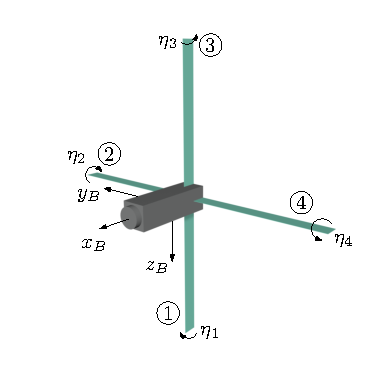
\includegraphics[scale=1]{Figures/fig1.eps}
			\caption{SOAR satellite geometry with body coordinate frame and control fin definitions.}
			\label{fig:satellite}
	\end{figure}

    Key model parameters are summarized in \Cref{tab:soar_parameters}. 
		% small table:
		\begin{table}[ht]
			%\centering
			\caption{Reference satellite model parameters (taken from \cite{livadiottiApplicationOrbitalAerodynamics2021}).}	
			\footnotesize{
			\begin{tabular}{lll}
				\hline
				\textbf{Parameter}      & \textbf{Value} & \textbf{Unit} \\
				\hline
				mass $m$              			& 2.877 & kg \\
				Body length $l_x$     			& 0.340 & m\\
				Panel length $l_{\text{p}}$     		& 0.570 & m\\
				Panel area (one side) $A_{\text{p}}$   & 0.0342 & m$^2$\\
				Inertia Matrix $J$  & $\text{diag} \left(
				\begin{bmatrix}0.0288 \\ 0.0392 \\ 0.0392
				\end{bmatrix}\right)$ & $\text{kg m}^2$\\
				distance CoM to rear& 0.161 & m\\
				\hline& 
			\end{tabular}
			\label{tab:soar_parameters}
			}
		\end{table}
		The commanded control fin angles are denoted with $\eta_1$ to $\eta_4$ and are equal to zero in the minimum-drag configuration.

    \subsection{Coordinate Frames}
		\begin{figure}[h]
            \centering
			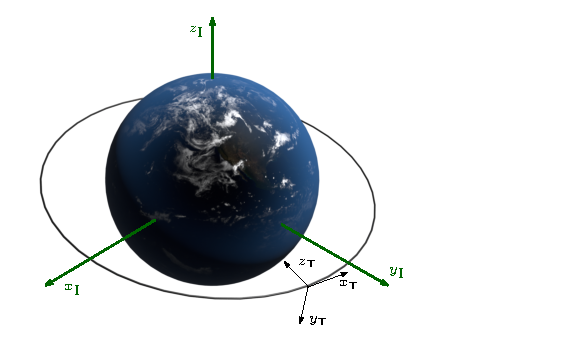
\includegraphics[scale=1]{Figures/fig2.eps}
			\caption{Tangential and ECI coordinate frame definitions.} %Fix explainer text here. Potentially add ECI frame in figure
			\label{fig:tangential_coordinate_frame}
		\end{figure}
		
		The coordinate frames are listed in \Cref{tab:frames}.
		To simplify aerodynamic calculations, we use the tangential frame $\text{T}$ as its axis $x_{\text{T}}$ points in the direction of the satellite's velocity as shown in \Cref{fig:tangential_coordinate_frame}.
		Furthermore, $y_{\text{T}}$ is aligned parallel to the negative orbital angular momentum and $z_{\text{T}}$ completes the right hand system.
		For a circular orbit, $z_{\text{T}}$ is aligned with the negative radial direction and the tangential frame is equal to local-vertical local-horizontal frame (LVLH).
		The corresponding unit vectors in the body frame are denoted by $x^{\text{B}}_{\text{T}}, y^{\text{B}}_{\text{T}}$ and $z^{\text{B}}_{\text{T}}$ respectively.

		\begin{table}[h]
			\renewcommand{\arraystretch}{1.1}
			\begin{tabular}{c p{6cm}} % Two columns: Symbol and Description
				\hline
				\textbf{Frame} & \textbf{Description} \\ \hline
				$\text{I}$     & Earth-centered inertial (ECI) frame: fixed relative to distant stars. \\
				$\text{B}$     & Body frame: aligned with the satellite's principal axes. \\
				$\text{T}$     & Tangential frame: aligned with the satellite's velocity direction. \\ \hline
			\end{tabular}
			\caption{Relevant coordinate frames.}
			\label{tab:frames}
		\end{table}

        \subsection{Kinematics}
		We define the quaternion
		\begin{equation}
			q = \begin{bmatrix}
				q_1 \\ q_2 \\q_3 \\ q_4
			\end{bmatrix}
			=
			\begin{bmatrix}
				q_\text{v} \\ q_4
			\end{bmatrix}
		\end{equation}
		with the scalar part $q_4$ and the vector part $q_\text{v}$. 
		Using this parametrization, the kinematic relationship between the angular velocity of the satellite and the time derivative of the quaternion describing the attitude of the satellite with respect to the tangential frame according to \cite{fichterPrinciplesSpacecraftControl2023} is given by
		% Quaternion kinematics
			\begin{equation}
				\label{eq:quaternion_kinematics}
				\dot{q}_{\text{BT}} = \frac{1}{2}\begin{bmatrix}
					-[\omega^{\text{B}}_{\text{BT}} \times] & \omega^{\text{B}}_{\text{BT}} \\
					-(\omega_{\text{BT}}^{\text{B}})^{\top} & 0
				\end{bmatrix}q_{\text{BT}}
			\end{equation}
		where $\omega_{\text{BT}}^{\text{B}}$ denotes the angular velocity of the satellite with respect to the tangential frame in body-fixed coordinates.

		The satellite's angular velocity with respect to the inertial frame expressed in the body frame is given by
		\begin{equation}
			\omega_{\text{BI}}^{\text{B}} = \omega_{\text{BT}}^{\text{B}} + \omega_{\text{TI}}^{\text{B}} 
			= \omega_{\text{BT}}^{\text{B}} + T_{\text{BT}}\omega_{\text{TI}}^{\text{T}}.
		\end{equation}
		where for a circular orbit, the angular velocity of the tangential frame relative to the inertial frame is given by $\omega_{\text{TI}}^{\text{T}} = \begin{bmatrix}
			0 & -\omega_0 & 0
		\end{bmatrix}^{\top}$ with the constant orbit rate $\omega_0$. Furthermore, using the Direction Cosine Matrix (DCM) 
		\begin{equation}
			T_{\text{BT}} = \begin{bmatrix}
				x^{\text{B}}_{\text{T}} & y^{\text{B}}_{\text{T}} & z^{\text{B}}_{\text{T}},
			\end{bmatrix}
		\end{equation}
		we obtain the simplified expression
		\begin{equation}
			\label{eq:inertial_rate_circular_orbit}
			\omega_{\text{BI}}^{\text{B}} = \omega_{\text{BT}}^{\text{B}} - \omega_0 y^{\text{B}}_{\text{T}}.
		\end{equation}


    \subsection{Dynamics}
		Using Euler's equation, we express the dynamics of the rigid body satellite with
		\begin{equation}
			\label{eq:dynamics}
			J \dot{\omega}_{\text{BI}}^{\text{B}} = -[\omega_{\text{BI}}^{\text{B}}\times] J \omega_{\text{BI}}^{\text{B}} + \tau_{\text{aero}}.
		\end{equation}

		Here, the aerodynamic torque $\tau_{\text{aero}}$ is assumed to be the only external torque acting on the satellite.
		By inserting \cref{eq:inertial_rate_circular_orbit} into \cref{eq:dynamics}, we obtain

		\begin{equation}
			J \left( \dot{\omega}_{\text{BT}}^{\text{B}}  - \omega_0 \dot{y}^{\text{B}}_{\text{T}} \right)
			= -\left(\omega_{\text{BT}}^{\text{B}} - \omega_0 y^{\text{B}}_{\text{T}}\right)
			\quad \times J \left(\omega_{\text{BT}}^{\text{B}} - \omega_0 y^{\text{B}}_{\text{T}}\right) + \tau_{\text{aero}}
			\label{eq:dynamics_inserted}
		\end{equation}

		which we simplify to obtain the final dynamics expressed in the body frame with

		\begin{equation}
			\begin{split}
			J \dot{\omega}_{\text{BT}}^{\text{B}} 
			= \left(J\omega_{\text{BT}}^{\text{B}} \right) \times \omega_{\text{BT}}^{\text{B}} 
			+ \omega_0 \omega_{\text{BT}}^{\text{B}} \times \left( J y^{\text{B}}_{\text{T}} \right)
			+ \omega_0 y^{\text{B}}_{\text{T}} \times \left( J \omega_{\text{BT}}^{\text{B}}\right) \\
			- \omega_0^2 \left(  y^{\text{B}}_{\text{T}}  
				\times 
				\left( J \omega_{\text{BT}}^{\text{B}} \right)  \right)
			- \omega_0 J \left(  \omega_{\text{BT}}^{\text{B}} \times y^{\text{B}}_{\text{T}} \right) 
			+ \tau_{\text{aero}}.
			\end{split}
			\label{eq:dynamics_orbit_frame}
		\end{equation}

		Introducing the state vector $x = \begin{bmatrix}
			q_{\text{BT}} & \omega_{\text{BT}}^{\text{B}}\end{bmatrix}^{\top}$ and the input vector $u = \tau_{\text{aero}}$, the system dynamics and kinematics can be expressed in the form of an input affine nonlinear state space representation as

		\begin{equation}
			\begin{aligned}
				\dot{x} &= f(x) + g(x)u, \\
			\end{aligned}
		\end{equation}
 
		where the vector fields $f$ and $g$ are defined by \cref{eq:quaternion_kinematics} and \cref{eq:dynamics_orbit_frame}. In this representation it is assumed that the aerodynamic torque $\tau_{\text{aero}}$ can be arbitrarily realized using rotating fins. While this assumption can be used to design the outer loop control law, significant limitations and nonlinear behaviour are introduced to the system when modelling the aerodynamics, which we aim to address in the following sections.



        \subsection{Aerodynamics}
		\label{sec:aerodynamics}
		To model the diffuse re-emission of particles from the satellite's surface, we employ the gas surface interaction model derived by Sentman \cite{sentman_free_1961}. The force exerted onto a single sided flat plate is given by
		\newcommand{\ii}{\text{i}}
		\newcommand{\pp}{\text{p}}
		\newcommand{\cosd}{\cos \delta}
		\begin{alignat}{2}
            \label{eq:plate_force_sentman}
			f_\text{p} 
			&= \frac{\rho}{2} A_\pp V_\ii^2 C &&\nonumber\\
			&= \frac{\rho}{2} A_\pp V_\ii^2\frac{1}{s_\ii^2}
			&&\Bigg[
				- \Gamma_1(s_\ii \cosd) \hat{n}_\pp \Bigg.
				- \frac{\sqrt{\pi}}{2} \sqrt{\frac{T_\text{r}}{T_\ii}} \Gamma_2(s_\ii \cosd) \hat{n}_\pp
				\Bigg.\\ \nonumber
                &&& + s_\ii \Gamma_2(s_\ii \cosd) \left(\hat{v}_\ii + \cosd ~\hat{n}_\pp\right)
			\Bigg]
		\end{alignat}

		where
		\begin{align*}
			\Gamma_1(\xi) &= \frac{\xi}{\sqrt{\pi}} \exp (-\xi^2) + \left(\frac{1}{2} + \xi^2 \right) \text{erfc} (-\xi) \\
			\Gamma_2(\xi) &= \frac{1}{\sqrt{\pi}} \exp (-\xi^2) + \xi \text{ erfc}(-\xi) \\
			\text{erfc}(z) &= \frac{2}{\sqrt{\pi}} \int_{z}^{\infty}e^{-\mu^2} \mathrm{d}\mu
		\end{align*}
		with the incoming particle velocity magnitude $V_\ii = \frac{v_\ii}{\hat{v}_\ii}$, the outward facing panel normal vector $\hat{n}_\pp$, the panel area $A_\pp$, the total mass density $\rho$, the molecular speed ratio $s_\ii$ and the angle between the normal vector and the incoming velocity direction $\delta$ for which the following holds:
		\begin{equation}
			\cosd = - \langle \hat{n}_\pp \; , \; \hat{v}_\ii \rangle.
		\end{equation}

		As shown in \cite{tuttasGeneralizedTreatmentEnergy2025a}, the temperature ratio can then be obtained for the general case with

		\begin{align}
			\begin{split}
				\frac{T_\mathrm{r}}{T_\mathrm{i}} &= \alpha_\mathrm{E} \frac{2 k T_\mathrm{w}}{m V_\mathrm{i}^2} s_{\text{i}}^2
                + \left( 1 - \alpha_\mathrm{E} \right) 
                \bigg(
					1 + \frac{s^2}{2} \\ & 
                    + \frac{1}{4} \frac{ s_{\text{i}} \cos\delta \text{ erfc}\left( - s_{\text{i}} \cos\delta \right) }{\frac{1}{\sqrt{\pi}} \exp \left( - s_{\text{i}}^2 \cos^2\delta \right) + s_{\text{i}} \cos\delta \text{ erfc}\left( - s_{\text{i}} \cos\delta \right)}
				\bigg)
			\end{split}
		\end{align}
		where $\alpha_E$ denotes the energy accommodation coefficient. Generally, it is assumed to be within the range of $0.9$ to $1$ for VLEO applications \cite{moe_gassurface_2005}.

		Applying \cref{eq:plate_force_sentman} to a two-sided control fin of the reference satellite results in the drag ($f_x$) and lift ($f_z$) forces shown in \Cref{fig:linearization}. The Taylor approximations of these forces around $\delta = 0$, corresponding to the satellite's nominal low-drag configuration, are represented by the dotted lines.
		While the linearization of the lift force (blue) remains accurate for angles up to approximately $15^\circ$, the constant approximation of the symmetric drag force (red) is valid over a significantly smaller range. Given the substantially higher magnitude of the drag force compared to the lift force, this indicates that the regions of validity for linearized aerodynamic models around the nominal configuration are severely limited in feather design configurations.


		% figure for linearization
		\begin{figure}[t]
			\centering
			\begin{tikzpicture}
	\begin{axis}[
		width=\columnwidth*0.6,
		xlabel={$\delta$ [deg]},
		ylabel={$f$ [N]},
		xmin=-1.57,xmax=1.57,  % This is approximately -90 to 90 degrees in radians<
		xtick={-1.57, -1.047, -0.524, 0, 0.524, 1.047, 1.57},
		xticklabels={-90, -60, -30, 0, 30, 60, 90},
		legend style={font=\footnotesize, at={(1.02,0.5)}, anchor=west, legend columns=1},
		]
		\addplot [blue,line width=1pt] table[x=alpha,y=lift__N] {Figures/data/linearization_drag_lift.dat};
		\addlegendentry{$f_z$ [N]}

		\addplot [red,line width=1pt] table[x=alpha,y=drag__N] {Figures/data/linearization_drag_lift.dat};
		\addlegendentry{$f_x$ [N]}

		\addplot [blue,dashed] table[x=alpha,y=liftLin__N] {Figures/data/linearization_drag_lift.dat};
		\addlegendentry{$f_{z, \mathrm{lin}}$ [N]}

		\addplot [red,dashed] table[x=alpha,y=dragLin__N] {Figures/data/linearization_drag_lift.dat};
		\addlegendentry{$f_{x, \mathrm{lin}}$ [N]}
	\end{axis}
\end{tikzpicture}
			\caption{Lift and drag over $\delta$ of a two-sided steering fin of the SOAR geometry for $\alpha_E=0.95$ at $300\,\text{km}$ altitude. Dotted lines indicate the linearization around $\delta=0$.}
			\label{fig:linearization}
		\end{figure}
		

		\subsubsection{Control Authority}
		Due to the short time horizons of attitude control compared to orbit control, the incident flow velocity \(V_\text{i}\), energy accommodation coefficient \(\alpha_E\), and molecular speed ratio \(s\) are assumed constant for the analysis in this section. Under this assumption, the aerodynamic torque in the body frame is expressed as a function of the incoming particle velocity direction and the panel normals:
		\begin{equation}
		\begin{aligned}
			\tau_{\text{aero}}(\hat{n}_i, \hat{v}_\text{i}) &= \sum_{i=1}^{4} r_{\text{p},i}\times f_i(\hat{n}_{\text{p},i},\hat{v}_\ii) \\  
			&= A_{\text{p}}\frac{\rho}{2} V_\ii^2 \sum_{i=1}^{4} r_{\text{p},i}\times C_i(\hat{n}_{\text{p},i},\hat{v}_\ii)
		\end{aligned}
		\label{eq:torque_simplified}
		\end{equation}
		where $f_i$ denotes the force generated by the $i$-th two-sided control fin in body coordinates and $r_{\text{p},i}$ is the distance vector from the center of mass to the center of pressure of the $i$-th control fin.
		Under the assumption that the relative velocity of the incoming particles predominantly stems from the satellite's own velocity, its direction is parallel to the negative x-axis of the tangential frame.
		It can therefore be parametrized using attitude quaternions with

		\begin{equation}
			\hat{v}_\ii = -\begin{bmatrix}
				2(q_4^2+q_1^2)-1 \\ 2(q_1q_2 -q_4q_3) \\ 2(q_1q_3 + q_4q_2)
			\end{bmatrix}
			\label{eq:quat_to_flow}
		\end{equation}

		where $q=q_{\text{BT}}$.
		In \Cref{fig:torque_envelope}, the achievable torque envelope for varying control fin angles is shown for a satellite facing the incoming flow directly.
		%In nominal flow configuration with $v_\ii$ aligning with the negative $x_B$ axis, the achievable torque envelope for varying control fin angles is shown in \Cref{fig:torque_envelope}.
		It can be seen that torque magnitudes in pitch ($\tau_y$) and yaw ($\tau_z$) clearly dominate roll ($\tau_x$) due to the low lift-to-drag ratio. 
		For complete panel rotations ($-90^{\circ} \leq \eta \leq 90^{\circ}$), the achievable torque spans a potentially convex volume.
		Since low drag magnitudes are desirable, control fin angles can be limited.
		As shown in \Cref{fig:torque_envelope} (right), this results in a nonconvex and highly complex torque envelope. Furthermore, these envelopes vary with  the satellite attitude, resulting in a challenging nonlinear allocation problem.

		\begin{figure*}[htbp]
			\centering
			\begin{minipage}{0.48\textwidth}
				\centering
				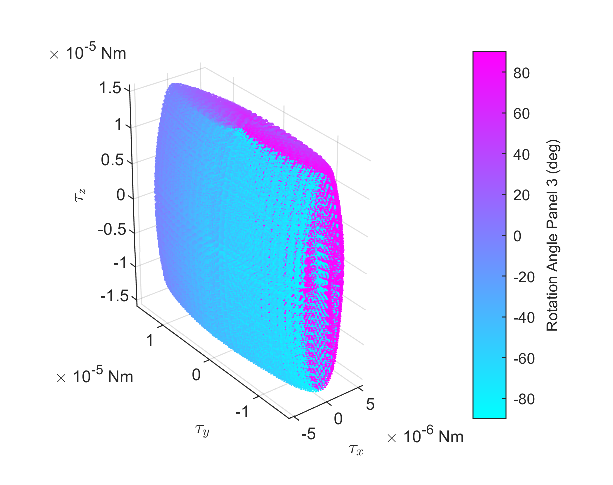
\includegraphics[width=\linewidth]{Figures/fig4.eps}
			\end{minipage}%
			\hfill
			\begin{minipage}{0.48\textwidth}
				\centering
				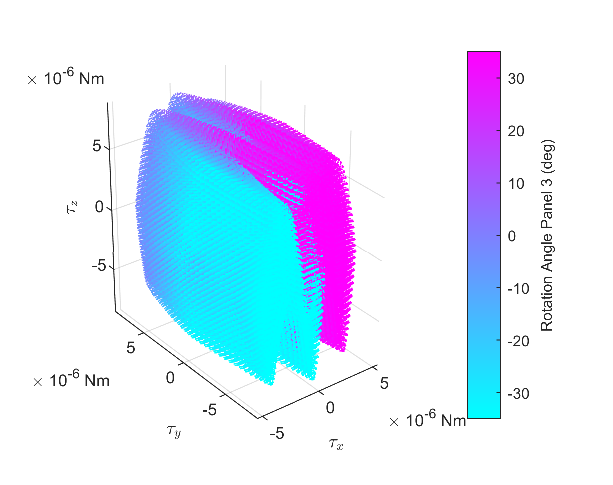
\includegraphics[width=\linewidth]{Figures/fig5.eps}
			\end{minipage}
			\caption{Point cloud plot approximation of active aerodynamic torque envelope. Each point represents a torque resulting from a variation of all four panel angles $\eta$. The color grading represents the rotation angle of one active control fin. Left: Control fin rotations up to $\pm 90^{\circ}$, Right: Control fin rotations limited to $\pm 35^{\circ}$.}
			\label{fig:torque_envelope}
		\end{figure*}


        \subsection{Time Variation and Uncertainty}
		\label{sec:uncertainty}
		The nonlinearities introduced by Sentman’s model are further compounded by the difficulty in validating its assumptions, as key parameters like the accommodation coefficient are derived from imperfect orbit data \cite{moeImprovedSatelliteDrag1998}. 
		Additionally, parameters such as the total mass density not only vary over time throughout orbits but also exhibit significant uncertainty. This is illustrated in \Cref{fig:density_uncertainty_over_orbit}, where the density values over an equatorial orbit are plotted with 1-$\sigma$ uncertainty based on the model developed by Boniface \cite{bonifaceUncertaintyQuantificationDTM20202021}.
		\begin{figure}[ht]
			\centering
			% This file was created by matlab2tikz.
%
%The latest updates can be retrieved from
%  http://www.mathworks.com/matlabcentral/fileexchange/22022-matlab2tikz-matlab2tikz
%where you can also make suggestions and rate matlab2tikz.
%
\definecolor{mycolor1}{rgb}{0.00000,0.44700,0.74100}%
\definecolor{mycolor2}{rgb}{0.85000,0.32500,0.09800}%
\definecolor{mycolor3}{rgb}{0.92900,0.69400,0.12500}%
\definecolor{mycolor4}{rgb}{0.49400,0.18400,0.55600}%
%
\begin{tikzpicture}

\begin{axis}[%
width=8.656cm,
height=5cm,
at={(0cm,0cm)},
scale only axis,
xmin=-180,
xmax=180,
xtick={-180, -120,  -60,    0,   60,  120,  180},
xlabel style={font=\color{white!15!black}},
xlabel={Longitude [$^{\circ}$]},
ymin=0,
ymax=1e-10,
ylabel style={font=\color{white!15!black}},
ylabel={$\text{Density (kg/m}^\text{3}\text{)}$},
axis background/.style={fill=white},
axis x line*=bottom,
axis y line*=left,
xmajorgrids,
ymajorgrids,
legend style={at={(0.5,0.97)}, legend columns=2, anchor=north, legend cell align=left, align=left, draw=white!15!black}
]

\addplot[area legend, draw=none, fill=mycolor1, fill opacity=0.2, forget plot]
table[row sep=crcr] {%
x	y\\
-177.027620181616	9.19704999179304e-11\\
-172.992909764763	9.29150281695708e-11\\
-168.95819918956	9.37971262482545e-11\\
-164.923488367124	9.45756095694616e-11\\
-160.888777211206	9.52123764285273e-11\\
-156.854065635817	9.56750468237456e-11\\
-152.819353557527	9.59378795384967e-11\\
-148.784640894948	9.59836676504577e-11\\
-144.74992757147	9.58050107893207e-11\\
-140.715213510498	9.54035745258262e-11\\
-136.680498642856	9.47900696247558e-11\\
-132.64578289966	9.39835509536049e-11\\
-128.611066219641	9.30090017419663e-11\\
-124.576348544333	9.18958771028284e-11\\
-120.541629820233	9.06764045434303e-11\\
-116.506910000917	8.93828626135929e-11\\
-112.472189042153	8.80461747809901e-11\\
-108.437466908647	8.66946833098134e-11\\
-104.402743569085	8.53524341945504e-11\\
-100.368018998159	8.40388061396959e-11\\
-96.3332931780673	8.27684128427991e-11\\
-92.2985660958462	8.15507310700116e-11\\
-88.2638377448018	8.039080119186e-11\\
-84.2291081264048	7.92900747305352e-11\\
-80.1943772451812	7.82470348242941e-11\\
-76.1596451151835	7.72584752968342e-11\\
-72.1249117548094	7.63206836268577e-11\\
-68.090177188576	7.54303360771906e-11\\
-64.0554414488455	7.45855319763602e-11\\
-60.0207045705551	7.37864135349426e-11\\
-55.9859665975574	7.3035423594998e-11\\
-51.95122757681	7.24843019285523e-11\\
-47.9164875623223	7.18771772099962e-11\\
-43.8817466116546	7.13368653956586e-11\\
-39.8470047874786	7.08705501809449e-11\\
-35.8122621563291	7.04838114639281e-11\\
-31.7775187906063	7.01800476710669e-11\\
-27.7427747630982	6.99594658502644e-11\\
-23.7080301531308	6.98182865576707e-11\\
-19.6732850410553	6.97494576885096e-11\\
-15.6385395097176	6.97429047775791e-11\\
-11.603793645897	6.97860197182888e-11\\
-7.56904753523898	6.98657794658608e-11\\
-3.53430126645412	6.99697769254746e-11\\
0.500445071876473	7.0087000226703e-11\\
4.53519138944023	7.02100199260511e-11\\
8.5699375974227	7.03352866163526e-11\\
12.6046836070845	7.04627754117184e-11\\
16.6394293306742	7.05971458100687e-11\\
20.6741746818592	7.07466672492338e-11\\
24.708919576614	7.09216410020888e-11\\
28.7436639317859	7.11349755247388e-11\\
32.7784076682973	7.14005647561006e-11\\
36.8131507101233	7.17315270634426e-11\\
40.8478929833133	7.21412782095829e-11\\
44.8826344191062	7.26422738737264e-11\\
48.9173749524349	7.32446781952893e-11\\
52.9521145231707	7.3958584881271e-11\\
56.9868530745753	7.47911084551391e-11\\
61.0215905563595	7.46466429336867e-11\\
65.0563269230739	7.52445988234791e-11\\
69.0910621348103	7.59404175947955e-11\\
70.0002398135435	7.68149950988205e-11\\
73.1257961573942	7.67287557014075e-11\\
74.0349737265792	7.81086889894722e-11\\
77.1605289630184	7.75995261848037e-11\\
78.0697064193828	7.81122961014116e-11\\
81.1952605275911	7.85373829940373e-11\\
82.1044378707741	7.90838885036682e-11\\
85.2299908378566	7.95207630671155e-11\\
86.1391680657239	8.00950899663205e-11\\
89.2647198821219	8.05223942708068e-11\\
90.1738969940598	8.11173504357271e-11\\
93.299447657314	8.15108061854158e-11\\
94.2086246533008	8.21182302644367e-11\\
98.2433510468061	8.30632005974537e-11\\
102.278076184233	8.39189977325851e-11\\
106.312800081951	8.46574296940828e-11\\
110.347522760635	8.52579793771842e-11\\
114.382244250282	8.5710620200399e-11\\
118.416964583545	8.60175542184072e-11\\
122.451683800699	8.61924481651917e-11\\
126.486401947101	8.62594584502023e-11\\
130.521119073456	8.6251280833183e-11\\
134.555835235529	8.62053183314099e-11\\
138.590550494362	8.61608216911799e-11\\
142.625264914101	8.61562070834795e-11\\
146.659978564461	8.62254711081011e-11\\
150.694691518532	8.63964206593228e-11\\
154.729403852869	8.66895255864687e-11\\
158.764115647582	8.71160050724117e-11\\
162.798826983613	8.7677765562959e-11\\
166.833537947442	8.83678384118437e-11\\
170.868248624142	8.91698626954009e-11\\
174.902959102567	9.00593336963661e-11\\
178.937669470677	9.10052536311169e-11\\
178.937669470677	6.68797096716823e-11\\
174.902959102567	6.59207485159807e-11\\
170.868248624142	6.50078324381835e-11\\
166.833537947442	6.41640187500791e-11\\
162.798826983613	6.34064648969922e-11\\
158.764115647582	6.27461689098525e-11\\
154.729403852869	6.21879771974971e-11\\
150.694691518532	6.17295210409788e-11\\
146.659978564461	6.13618434369057e-11\\
142.625264914101	6.10703275162055e-11\\
138.590550494362	6.08346569036571e-11\\
134.555835235529	6.06304970869645e-11\\
130.521119073456	6.04315238871354e-11\\
126.486401947101	6.02105109246131e-11\\
122.451683800699	5.99419358551743e-11\\
118.416964583545	5.96045803843344e-11\\
114.382244250282	5.91827171249072e-11\\
110.347522760635	5.86680404818998e-11\\
106.312800081951	5.80607897482588e-11\\
102.278076184233	5.73688716875357e-11\\
98.2433510468061	5.66072044566847e-11\\
94.2086246533008	5.57962113794766e-11\\
93.299447657314	5.59939627388214e-11\\
90.1738969940598	5.49588964572475e-11\\
89.2647198821219	5.51337264618734e-11\\
86.1391680657239	5.41188438553687e-11\\
85.2299908378566	5.42753993419233e-11\\
82.1044378707741	5.32983916567868e-11\\
81.1952605275911	5.34409468714583e-11\\
78.0697064193828	5.25165547694204e-11\\
77.1605289630184	5.26486666043903e-11\\
74.0349737265792	5.08830558463178e-11\\
73.1257961573942	5.19128166128643e-11\\
70.0002398135435	5.06839218121011e-11\\
69.0910621348103	5.12437615911697e-11\\
65.0563269230739	5.06477920264255e-11\\
61.0215905563595	5.01280274967955e-11\\
56.9868530745753	4.90420437831341e-11\\
52.9521145231707	4.9106453317748e-11\\
48.9173749524349	4.92189367319239e-11\\
44.8826344191062	4.93765898134618e-11\\
40.8478929833133	4.95764832470157e-11\\
36.8131507101233	4.98129178040276e-11\\
32.7784076682973	5.00798645150396e-11\\
28.7436639317859	5.03700758262045e-11\\
24.708919576614	5.06746069944687e-11\\
20.6741746818592	5.09850415860696e-11\\
16.6394293306742	5.12932101619115e-11\\
12.6046836070845	5.15912474601674e-11\\
8.5699375974227	5.18738499114368e-11\\
4.53519138944023	5.21381456044869e-11\\
0.500445071876473	5.2383592555582e-11\\
-3.53430126645412	5.26134352232634e-11\\
-7.56904753523898	5.28338526679744e-11\\
-11.603793645897	5.30529648120184e-11\\
-15.6385395097176	5.32810583170578e-11\\
-19.6732850410553	5.35289717583551e-11\\
-23.7080301531308	5.38066134730419e-11\\
-27.7427747630982	5.412278657692e-11\\
-31.7775187906063	5.44839105624819e-11\\
-35.8122621563291	5.48932583387523e-11\\
-39.8470047874786	5.53515239955523e-11\\
-43.8817466116546	5.58567338954815e-11\\
-47.9164875623223	5.64046566480162e-11\\
-51.95122757681	5.69901217663897e-11\\
-55.9859665975574	5.77231229016625e-11\\
-60.0207045705551	5.83364404019298e-11\\
-64.0554414488455	5.89734724955336e-11\\
-68.090177188576	5.96322479346392e-11\\
-72.1249117548094	6.03126255668617e-11\\
-76.1596451151835	6.10160350861172e-11\\
-80.1943772451812	6.17449465388603e-11\\
-84.2291081264048	6.25022732486618e-11\\
-88.2638377448018	6.3290343188831e-11\\
-92.2985660958462	6.41100643344996e-11\\
-96.3332931780673	6.49602811868561e-11\\
-100.368018998159	6.58367360974479e-11\\
-104.402743569085	6.67316649150804e-11\\
-108.437466908647	6.76337724701686e-11\\
-112.472189042153	6.85277584533475e-11\\
-116.506910000917	6.93948105190081e-11\\
-120.541629820233	7.02135544256487e-11\\
-124.576348544333	7.09603832813516e-11\\
-128.611066219641	7.16109333042201e-11\\
-132.64578289966	7.21419016500995e-11\\
-136.680498642856	7.25318618471744e-11\\
-140.715213510498	7.27631397588148e-11\\
-144.74992757147	7.28236555533334e-11\\
-148.784640894948	7.27072085125751e-11\\
-152.819353557527	7.24145956283784e-11\\
-156.854065635817	7.195432593574e-11\\
-160.888777211206	7.13414362803735e-11\\
-164.923488367124	7.05971696736192e-11\\
-168.95819918956	6.97482704039519e-11\\
-172.992909764763	6.88245284476156e-11\\
-177.027620181616	6.78575612620502e-11\\
}--cycle;
\addplot [color=mycolor1, line width=1.5pt]
  table[row sep=crcr]{%
-177.027620181616	7.99218469182961e-11\\
-172.992909764763	8.08597633294994e-11\\
-168.95819918956	8.17692580312723e-11\\
-164.923488367124	8.2593487604754e-11\\
-160.888777211206	8.32756086310837e-11\\
-156.854065635817	8.38156211102614e-11\\
-152.819353557527	8.41851033328567e-11\\
-148.784640894948	8.43556335894391e-11\\
-144.74992757147	8.43272118800087e-11\\
-140.715213510498	8.40714164951351e-11\\
-136.680498642856	8.36735125631094e-11\\
-132.64578289966	8.30766566650709e-11\\
-128.611066219641	8.230927051045e-11\\
-124.576348544333	8.14281975181075e-11\\
-120.541629820233	8.04334376880433e-11\\
-116.506910000917	7.93818344391184e-11\\
-108.437466908647	7.71649411035469e-11\\
-100.368018998159	7.49480477679754e-11\\
-96.3332931780673	7.386802280962e-11\\
-92.2985660958462	7.28164195606951e-11\\
-88.2638377448018	7.18500814400613e-11\\
-84.2291081264048	7.08837433194276e-11\\
-80.1943772451812	7.00026703270851e-11\\
-76.1596451151835	6.9150019044173e-11\\
-68.090177188576	6.75299816066399e-11\\
-60.0207045705551	6.60520527162589e-11\\
-55.9859665975574	6.53699316899292e-11\\
-51.95122757681	6.47446540824603e-11\\
-47.9164875623223	6.41477981844218e-11\\
-43.8817466116546	6.36077857052442e-11\\
-39.8470047874786	6.31246166449273e-11\\
-35.8122621563291	6.26982910034712e-11\\
-31.7775187906063	6.2328808780876e-11\\
-27.7427747630982	6.20445916865719e-11\\
-23.7080301531308	6.18172180111287e-11\\
-19.6732850410553	6.16466877545463e-11\\
-11.603793645897	6.14193140791031e-11\\
28.7436639317859	6.07656147622038e-11\\
32.7784076682973	6.07371930527734e-11\\
36.8131507101233	6.07656147622038e-11\\
40.8478929833133	6.0850879890495e-11\\
44.8826344191062	6.10214101470774e-11\\
48.9173749524349	6.12203621130902e-11\\
52.9521145231707	6.15330009168247e-11\\
56.9868530745753	6.19024831394199e-11\\
61.0215905563595	6.23856521997368e-11\\
65.0563269230739	6.29540863883449e-11\\
70.0002398135435	6.37498942523962e-11\\
74.0349737265792	6.44888586975867e-11\\
78.0697064193828	6.53130882710684e-11\\
85.2299908378566	6.6904703999171e-11\\
94.2086246533008	6.89510670781601e-11\\
98.2433510468061	6.98321400705026e-11\\
102.278076184233	7.06563696439844e-11\\
106.312800081951	7.13669123797445e-11\\
110.347522760635	7.19637682777829e-11\\
114.382244250282	7.24469373380998e-11\\
118.416964583545	7.28164195606951e-11\\
122.451683800699	7.30722149455687e-11\\
126.486401947101	7.32427452021511e-11\\
134.555835235529	7.34132754587336e-11\\
142.625264914101	7.36122274247464e-11\\
146.659978564461	7.37827576813288e-11\\
150.694691518532	7.40669747756328e-11\\
154.729403852869	7.44364569982281e-11\\
158.764115647582	7.4919626058545e-11\\
162.798826983613	7.55449036660139e-11\\
166.833537947442	7.6255446401774e-11\\
170.868248624142	7.70796759752557e-11\\
174.902959102567	7.79891706770286e-11\\
178.937669470677	7.89555087976623e-11\\
};
\addlegendentry{250 km}


\addplot[area legend, draw=none, fill=mycolor2, fill opacity=0.2, forget plot]
table[row sep=crcr] {%
x	y\\
-178.297877818372	3.40456275985876e-11\\
-174.308533647346	3.45653303963299e-11\\
-170.319189350891	3.50613402661112e-11\\
-166.32984484342	3.55180957966147e-11\\
-162.340500041772	3.59204303897046e-11\\
-158.351154862822	3.62539781375327e-11\\
-154.361809225748	3.65064120699566e-11\\
-150.372463051499	3.66676689099568e-11\\
-146.383116265504	3.6730942058097e-11\\
-142.393768792898	3.66926288275852e-11\\
-138.404420565898	3.65526240906376e-11\\
-134.415071516676	3.63143554496531e-11\\
-130.425721584657	3.59840846725387e-11\\
-126.436370711705	3.55707893554604e-11\\
-122.447018844268	3.50851243889992e-11\\
-118.457665935495	3.45390711377989e-11\\
-114.468311940341	3.39448683230257e-11\\
-110.478956822314	3.33146772270238e-11\\
-106.489600548521	3.26597496340527e-11\\
-102.500243091696	3.1990136888613e-11\\
-98.5108844317042	3.13145028796313e-11\\
-94.5215245528904	3.06398197568189e-11\\
-90.5321634455175	2.99716277987943e-11\\
-86.5428011076759	2.93140224389552e-11\\
-82.5534375401917	2.86701009966891e-11\\
-78.5640727531161	2.80421684427313e-11\\
-74.5747067605659	2.74322342244186e-11\\
-70.5853395825196	2.68422785169701e-11\\
-66.5959712465691	2.62746312504845e-11\\
-62.6066017826748	2.57321305740504e-11\\
-58.6172312295351	2.52182395682994e-11\\
-54.6278596288073	2.47783439154258e-11\\
-50.6384870290819	2.43439236429946e-11\\
-46.6491134824169	2.3950914733471e-11\\
-42.6597390459307	2.36035050932391e-11\\
-38.6703637805871	2.3305026182821e-11\\
-34.6809877532316	2.30577296321108e-11\\
-30.6916110311517	2.28622252136451e-11\\
-26.7022336882568	2.27174495314135e-11\\
-22.7128557996052	2.26205061890972e-11\\
-18.723477442905	2.25666181491678e-11\\
-14.7340986999885	2.25496542020267e-11\\
-10.744719651777	2.25621887240693e-11\\
-6.75534038251472	2.25963693135403e-11\\
-2.76596097660205	2.26440937150342e-11\\
1.22341847951041	2.2697992765245e-11\\
5.21279790052493	2.27514908588273e-11\\
9.20217720084426	2.27996767587896e-11\\
13.1915562954617	2.28390495339452e-11\\
17.1809351003684	2.28680734011619e-11\\
21.1703135334199	2.28869463932362e-11\\
25.1596915128845	2.28971870318167e-11\\
29.1490689606278	2.29019639409992e-11\\
33.1384458010786	2.29051828108894e-11\\
37.1278219602389	2.29119391790305e-11\\
41.1171973687901	2.29276014033948e-11\\
45.1065719605953	2.29584213160078e-11\\
49.0959456739375	2.30106499835299e-11\\
53.085318449976	2.30911639977512e-11\\
57.0746902358067	2.32070839157852e-11\\
61.0640609828605	2.30346480997018e-11\\
65.0534306476146	2.3100209035403e-11\\
69.0427991917981	2.32131024214426e-11\\
70.0002380198148	2.34560832992758e-11\\
73.0321665830402	2.33775269128212e-11\\
73.9896052866194	2.37743846019197e-11\\
77.0215327922402	2.35961207598228e-11\\
77.9789713696981	2.37468260655882e-11\\
81.0108978007061	2.38692563726403e-11\\
81.9683362486525	2.40390871421215e-11\\
85.0002615909084	2.41948248617352e-11\\
85.9576999089157	2.43828809040585e-11\\
88.9896241535627	2.45677610564491e-11\\
89.9470623404537	2.47725565723832e-11\\
93.9364235405993	2.51995678186669e-11\\
97.9257835122005	2.56531257700186e-11\\
101.915142264082	2.61207590125785e-11\\
105.904499811463	2.65896390438496e-11\\
109.89385617356	2.70475606588929e-11\\
113.88321137861	2.7484442737349e-11\\
117.872565457219	2.78931022156415e-11\\
121.861918447341	2.82700220154195e-11\\
125.851270391749	2.86157041133951e-11\\
129.840621338326	2.89341435465513e-11\\
133.829971339795	2.92325513929517e-11\\
137.819320453949	2.95201083895211e-11\\
141.808668741511	2.98072996604785e-11\\
145.798016268618	3.01044966094165e-11\\
149.787363104649	3.04213812512632e-11\\
153.77670932235	3.07657929478942e-11\\
157.766054997942	3.11432380005777e-11\\
161.75540020843	3.15566047695205e-11\\
165.74474503634	3.20055351891541e-11\\
169.734089562797	3.24867594527256e-11\\
173.723433872744	3.2993740107402e-11\\
177.712778050299	3.35173381710799e-11\\
177.712778050299	2.26728784174609e-11\\
173.723433872744	2.22293173159784e-11\\
169.734089562797	2.17995639505126e-11\\
165.74474503634	2.13899409288761e-11\\
161.75540020843	2.10045606610701e-11\\
157.766054997942	2.06456507335907e-11\\
153.77670932235	2.03131176489128e-11\\
149.787363104649	2.00050723999318e-11\\
145.798016268618	1.97176774344899e-11\\
141.808668741511	1.94456346298501e-11\\
137.819320453949	1.91827691793655e-11\\
133.829971339795	1.89222341161777e-11\\
129.840621338326	1.86575205465837e-11\\
125.851270391749	1.83827478311621e-11\\
121.861918447341	1.80936690381991e-11\\
117.872565457219	1.77878549903493e-11\\
113.88321137861	1.7465391835463e-11\\
109.89385617356	1.71286908492635e-11\\
105.904499811463	1.67824381500388e-11\\
101.915142264082	1.64332404176711e-11\\
97.9257835122005	1.60887087396846e-11\\
93.9364235405993	1.57569569107985e-11\\
89.9470623404537	1.54455708746674e-11\\
88.9896241535627	1.54820377758689e-11\\
85.9576999089157	1.51611984976679e-11\\
85.0002615909084	1.51985447761306e-11\\
81.9683362486525	1.49088544384693e-11\\
81.0108978007061	1.49481878381849e-11\\
77.9789713696981	1.46918940943166e-11\\
77.0215327922402	1.47337786840028e-11\\
73.9896052866194	1.42463649614187e-11\\
73.0321665830402	1.45564592246388e-11\\
70.0002380198148	1.42379557204468e-11\\
69.0427991917981	1.44156634505738e-11\\
65.0534306476146	1.43096175567096e-11\\
61.0640609828605	1.42354723896192e-11\\
57.0746902358067	1.39937064270304e-11\\
53.085318449976	1.41007250462872e-11\\
49.0959456739375	1.42222919658467e-11\\
45.1065719605953	1.43549236645212e-11\\
41.1171973687901	1.44950254945032e-11\\
37.1278219602389	1.46386885648039e-11\\
33.1384458010786	1.47824722037744e-11\\
29.1490689606278	1.49227107303374e-11\\
25.1596915128845	1.50563904349101e-11\\
21.1703135334199	1.51805891583898e-11\\
17.1809351003684	1.52933609274473e-11\\
13.1915562954617	1.5393285709773e-11\\
9.20217720084426	1.54802253972832e-11\\
5.21279790052493	1.55552213432055e-11\\
1.22341847951041	1.56203825059256e-11\\
-2.76596097660205	1.56793115532176e-11\\
-6.75534038251472	1.57364494362619e-11\\
-10.744719651777	1.57972877606113e-11\\
-14.7340986999885	1.58675689049765e-11\\
-18.723477442905	1.59532932556082e-11\\
-22.7128557996052	1.60599089759822e-11\\
-26.7022336882568	1.61922861283319e-11\\
-30.6916110311517	1.63540679919859e-11\\
-34.6809877532316	1.65477410148198e-11\\
-38.6703637805871	1.67744185971228e-11\\
-42.6597390459307	1.70338037534789e-11\\
-46.6491134824169	1.73245427155688e-11\\
-50.6384870290819	1.7644253491518e-11\\
-54.6278596288073	1.79900200264048e-11\\
-58.6172312295351	1.83900364221142e-11\\
-62.6066017826748	1.87680964392119e-11\\
-66.5959712465691	1.91625053398469e-11\\
-70.5853395825196	1.95705951968123e-11\\
-74.5747067605659	1.99901248112678e-11\\
-78.5640727531161	2.04192545572641e-11\\
-82.5534375401917	2.08563461132805e-11\\
-86.5428011076759	2.12998173325462e-11\\
-90.5321634455175	2.17477864458501e-11\\
-94.5215245528904	2.21979240477039e-11\\
-98.5108844317042	2.26470664063581e-11\\
-102.500243091696	2.3091191623919e-11\\
-106.489600548521	2.35251176872039e-11\\
-110.478956822314	2.39427019098368e-11\\
-114.468311940341	2.43367363077405e-11\\
-118.457665935495	2.46992335440561e-11\\
-122.447018844268	2.5021873901194e-11\\
-126.436370711705	2.52961431476644e-11\\
-130.425721584657	2.55141405629957e-11\\
-134.415071516676	2.56687416324183e-11\\
-138.404420565898	2.57544648859086e-11\\
-142.393768792898	2.57675245248846e-11\\
-146.383116265504	2.57065686204966e-11\\
-150.372463051499	2.55725130416292e-11\\
-154.361809225748	2.5368726893941e-11\\
-158.351154862822	2.51010750685673e-11\\
-162.340500041772	2.47772343929092e-11\\
-166.32984484342	2.44067325947451e-11\\
-170.319189350891	2.39999791177343e-11\\
-174.308533647346	2.35681663106493e-11\\
-178.297877818372	2.31222935388688e-11\\
}--cycle;
\addplot [color=mycolor2, line width=1.5pt]
  table[row sep=crcr]{%
-178.297877818372	2.85922396869864e-11\\
-170.319189350891	2.95301560981898e-11\\
-166.32984484342	2.99564817396458e-11\\
-162.340500041772	3.03543856716715e-11\\
-158.351154862822	3.06670244754059e-11\\
-154.361809225748	3.095124156971e-11\\
-150.372463051499	3.11217718262924e-11\\
-146.383116265504	3.12070369545836e-11\\
-142.393768792898	3.1235458664014e-11\\
-138.404420565898	3.11501935357228e-11\\
-134.415071516676	3.09796632791404e-11\\
-130.425721584657	3.07522896036971e-11\\
-126.436370711705	3.04396507999627e-11\\
-122.447018844268	3.0041746867937e-11\\
-118.457665935495	2.9615421226481e-11\\
-110.478956822314	2.86206613964168e-11\\
-102.500243091696	2.75406364380615e-11\\
-82.5534375401917	2.47553089138819e-11\\
-74.5747067605659	2.37037056649569e-11\\
-66.5959712465691	2.27089458348928e-11\\
-58.6172312295351	2.17994511331199e-11\\
-50.6384870290819	2.10036432690686e-11\\
-42.6597390459307	2.03215222427389e-11\\
-38.6703637805871	2.00373051484348e-11\\
-34.6809877532316	1.98099314729916e-11\\
-30.6916110311517	1.96109795069788e-11\\
-26.7022336882568	1.94688709598267e-11\\
-18.723477442905	1.92699189938139e-11\\
-10.744719651777	1.91846538655227e-11\\
17.1809351003684	1.90709670278011e-11\\
29.1490689606278	1.89004367712187e-11\\
45.1065719605953	1.8644641386345e-11\\
53.085318449976	1.85877979674842e-11\\
61.0640609828605	1.8644641386345e-11\\
65.0534306476146	1.87014848052058e-11\\
70.0002380198148	1.88435933523579e-11\\
73.9896052866194	1.90141236089403e-11\\
77.9789713696981	1.92130755749531e-11\\
81.9683362486525	1.94688709598267e-11\\
88.9896241535627	2.00373051484348e-11\\
93.9364235405993	2.04920524993213e-11\\
105.904499811463	2.16857642953983e-11\\
113.88321137861	2.24815721594496e-11\\
121.861918447341	2.31921148952097e-11\\
129.840621338326	2.37889707932482e-11\\
149.787363104649	2.52100562647684e-11\\
157.766054997942	2.58921772910981e-11\\
165.74474503634	2.66879851551494e-11\\
173.723433872744	2.75974798569223e-11\\
177.712778050299	2.81090706266696e-11\\
};
\addlegendentry{300 km}


\addplot[area legend, draw=none, fill=mycolor3, fill opacity=0.2, forget plot]
table[row sep=crcr] {%
x	y\\
-179.544489395869	1.42034364187193e-11\\
-175.599666960235	1.44833529612095e-11\\
-171.654844429808	1.47535759288609e-11\\
-167.710021722195	1.50079271392165e-11\\
-163.76519875725	1.52400103019817e-11\\
-159.820375454652	1.54434198490383e-11\\
-155.875551736155	1.56122000128193e-11\\
-151.93072752503	1.57410583806064e-11\\
-147.985902748764	1.58256931348163e-11\\
-144.041077334253	1.58629308419811e-11\\
-140.096251215181	1.58510264310477e-11\\
-136.151424324858	1.57896457920291e-11\\
-132.206596603522	1.56798934185718e-11\\
-128.261767993504	1.55241241814599e-11\\
-124.316938441373	1.53258825346144e-11\\
-120.372107900037	1.50895736784025e-11\\
-116.427276323854	1.48202203167119e-11\\
-112.482443675371	1.45231082819102e-11\\
-108.537609920371	1.42036140239197e-11\\
-104.592775029906	1.3866903052478e-11\\
-100.647938981807	1.35177784947516e-11\\
-96.7031017580375	1.3160519326939e-11\\
-92.7582633461409	1.27989003739308e-11\\
-88.8134237411653	1.24361563312748e-11\\
-84.8685829405846	1.20750592113362e-11\\
-80.9237409508034	1.17180275619078e-11\\
-76.9788977820161	1.13672320447413e-11\\
-73.0340534500238	1.10247579054547e-11\\
-69.0892079780074	1.06926955420572e-11\\
-65.1443613913075	1.03732281885615e-11\\
-61.1995137238186	1.00686649131188e-11\\
-57.2546650122362	9.79459583670233e-12\\
-53.3098153000611	9.5306846299418e-12\\
-49.3649646341618	9.28887971168319e-12\\
-45.4201130663973	9.07139453117656e-12\\
-41.475260652434	8.88004307957047e-12\\
-37.530407453814	8.71610603065259e-12\\
-33.5855535325457	8.58017056976777e-12\\
-29.6406989573191	8.47206904229231e-12\\
-25.6958437980623	8.39075364081493e-12\\
-21.750988127477	8.33433590967212e-12\\
-17.8061320225439	8.30013183906716e-12\\
-13.8612755595197	8.28475948794238e-12\\
-9.91641881820042	8.28437348205108e-12\\
-5.97156187878698	8.29477807125441e-12\\
-2.02670482380752	8.31172899667836e-12\\
1.91815226505958	8.33114019037202e-12\\
5.86300930550517	8.34939933322854e-12\\
9.80786621545534	8.36343289809765e-12\\
13.7527229134549	8.37093110778866e-12\\
17.6975793195139	8.37038093803145e-12\\
21.6424353536358	8.36119554048687e-12\\
25.5872909389864	8.3435248436997e-12\\
29.5321460008428	8.31829462833436e-12\\
33.4770004655941	8.287061601546e-12\\
37.4218542638352	8.25205015634505e-12\\
41.3667073288623	8.21587574466689e-12\\
45.3115595979082	8.18159600907034e-12\\
49.2564110105951	8.15261468698968e-12\\
53.2012615119965	8.13258160233748e-12\\
57.1461110510392	8.12547783667186e-12\\
61.090959581221	8.02338050559302e-12\\
65.0358070608256	8.00756754717205e-12\\
68.9806534535837	8.01421962151512e-12\\
70.0002362526939	8.0896179700748e-12\\
72.9254987260551	8.04641667054086e-12\\
73.9450813843373	8.17512931481449e-12\\
76.8703428547891	8.10665433442156e-12\\
77.8899253674055	8.1569509446405e-12\\
80.8151858170939	8.19660973892614e-12\\
81.8347681822489	8.25679681779197e-12\\
84.7600275981463	8.31696857882654e-12\\
85.7796098147492	8.38710317992779e-12\\
89.7244502550165	8.54709521057407e-12\\
93.6692895002219	8.73473825771877e-12\\
97.6141275527457	8.94679688936777e-12\\
101.558964420642	9.17895752658072e-12\\
105.503800118059	9.42618135306741e-12\\
109.448634662853	9.68306270955373e-12\\
113.393468081614	9.94431684103856e-12\\
117.338300403033	1.02051956109595e-11\\
121.283131662881	1.04619751232394e-11\\
125.227961901509	1.07121926279551e-11\\
129.172791164147	1.09548085650401e-11\\
133.117619500649	1.1190108148831e-11\\
137.06244696575	1.14196158995474e-11\\
141.007273616942	1.16457371633697e-11\\
144.95209951698	1.18714126096798e-11\\
148.896924731736	1.20997551507129e-11\\
152.841749330344	1.2333611462044e-11\\
156.786573385339	1.25753369595386e-11\\
160.731396969985	1.28264843685843e-11\\
164.676220163043	1.30876335866893e-11\\
168.621043041874	1.33581872607931e-11\\
172.565865687685	1.36364440486539e-11\\
176.510688180916	1.39195263356433e-11\\
176.510688180916	8.65556801556807e-12\\
172.565865687685	8.44527862544267e-12\\
168.621043041874	8.23936945757147e-12\\
164.676220163043	8.03963227838572e-12\\
160.731396969985	7.8471386161603e-12\\
156.786573385339	7.66216292426323e-12\\
152.841749330344	7.48435800062358e-12\\
148.896924731736	7.31275576501049e-12\\
144.95209951698	7.14594678341004e-12\\
141.007273616942	6.98215458090306e-12\\
137.06244696575	6.81955995070546e-12\\
133.117619500649	6.6564402100252e-12\\
129.172791164147	6.49141247452441e-12\\
125.227961901509	6.32365542216612e-12\\
121.283131662881	6.15300770786887e-12\\
117.338300403033	5.98015779048921e-12\\
113.393468081614	5.80658348262816e-12\\
109.448634662853	5.63449023583737e-12\\
105.503800118059	5.46658029961967e-12\\
101.558964420642	5.3058893092406e-12\\
97.6141275527457	5.15546039339895e-12\\
93.6692895002219	5.01810438907635e-12\\
89.7244502550165	4.89613861214304e-12\\
85.7796098147492	4.79129305058153e-12\\
84.7600275981463	4.80065763620776e-12\\
81.8347681822489	4.70458711255349e-12\\
80.8151858170939	4.71661434170518e-12\\
77.8899253674055	4.6363367325447e-12\\
76.8703428547891	4.65105841083953e-12\\
73.9450813843373	4.49821552004683e-12\\
72.9254987260551	4.6034674665461e-12\\
70.0002362526939	4.5095481052512e-12\\
68.9806534535837	4.5727554374384e-12\\
65.0358070608256	4.55740647869171e-12\\
61.090959581221	4.55556499080886e-12\\
57.1461110510392	4.49786257132088e-12\\
53.2012615119965	4.55969066459986e-12\\
49.2564110105951	4.62713367806665e-12\\
45.3115595979082	4.6982593497643e-12\\
41.3667073288623	4.77103099669003e-12\\
37.4218542638352	4.84351558348611e-12\\
33.4770004655941	4.91389833017926e-12\\
29.5321460008428	4.98050811052864e-12\\
25.5872909389864	5.04200703763018e-12\\
21.6424353536358	5.09727102208941e-12\\
17.6975793195139	5.14559415022365e-12\\
13.7527229134549	5.18670374170086e-12\\
9.80786621545534	5.22092652087969e-12\\
5.86300930550517	5.24906561042882e-12\\
1.91815226505958	5.27251108772671e-12\\
-2.02670482380752	5.29315331379228e-12\\
-5.97156187878698	5.31338508720387e-12\\
-9.91641881820042	5.33585317300314e-12\\
-13.8612755595197	5.36339515469834e-12\\
-17.8061320225439	5.39883652097402e-12\\
-21.750988127477	5.44488931219136e-12\\
-25.6958437980623	5.50390308552905e-12\\
-29.6406989573191	5.57780652400981e-12\\
-33.5855535325457	5.66800072800749e-12\\
-37.530407453814	5.77529886580983e-12\\
-41.475260652434	5.89996106219673e-12\\
-45.4201130663973	6.04165957592978e-12\\
-49.3649646341618	6.19959007949793e-12\\
-53.3098153000611	6.3725463563847e-12\\
-57.2546650122362	6.55905747549507e-12\\
-61.1995137238186	6.76700477000922e-12\\
-65.1443613913075	6.97183545154859e-12\\
-69.0892079780074	7.18499550436115e-12\\
-73.0340534500238	7.40482601124808e-12\\
-76.9788977820161	7.62975412461848e-12\\
-80.9237409508034	7.85826999378852e-12\\
-84.8685829405846	8.08888228778464e-12\\
-88.8134237411653	8.32002219837841e-12\\
-92.7582633461409	8.54999349076083e-12\\
-96.7031017580375	8.77687172125898e-12\\
-100.647938981807	8.99844494290795e-12\\
-104.592775029906	9.21218905787716e-12\\
-108.537609920371	9.41521892249614e-12\\
-112.482443675371	9.60439949253004e-12\\
-116.427276323854	9.77638466060309e-12\\
-120.372107900037	9.9277706317353e-12\\
-124.316938441373	1.0055186946442e-11\\
-128.261767993504	1.01555770040103e-11\\
-132.206596603522	1.02263206204774e-11\\
-136.151424324858	1.02654489748807e-11\\
-140.096251215181	1.02717110853551e-11\\
-144.041077334253	1.02448053457033e-11\\
-147.985902748764	1.01853499988413e-11\\
-151.93072752503	1.00949188603122e-11\\
-155.875551736155	9.97588006206373e-12\\
-159.820375454652	9.83141400380014e-12\\
-163.76519875725	9.66525685913595e-12\\
-167.710021722195	9.48155493310333e-12\\
-171.654844429808	9.28456331715773e-12\\
-175.599666960235	9.07858335630175e-12\\
-179.544489395869	8.86767419772851e-12\\
}--cycle;
\addplot [color=mycolor3, line width=1.5pt]
  table[row sep=crcr]{%
-179.544489395869	1.1539214028744e-11\\
-167.710021722195	1.22497567645041e-11\\
-159.820375454652	1.26476606965298e-11\\
-151.93072752503	1.29318777908338e-11\\
-147.985902748764	1.3017142919125e-11\\
-144.041077334253	1.30455646285554e-11\\
-140.096251215181	1.30739863379858e-11\\
-136.151424324858	1.3017142919125e-11\\
-132.206596603522	1.29602995002642e-11\\
-124.316938441373	1.27045041153906e-11\\
-116.427276323854	1.23066001833649e-11\\
-108.537609920371	1.18234311230481e-11\\
-96.7031017580375	1.09707798401359e-11\\
-69.0892079780074	8.95283847057726e-12\\
-57.2546650122362	8.18545231595635e-12\\
-49.3649646341618	7.73070496506989e-12\\
-41.475260652434	7.38964445190504e-12\\
-33.5855535325457	7.13384906703141e-12\\
-25.6958437980623	6.93489710101858e-12\\
-17.8061320225439	6.84963197272737e-12\\
-5.97156187878699	6.79278855386656e-12\\
17.6975793195139	6.76436684443615e-12\\
29.5321460008428	6.65068000671454e-12\\
61.090959581221	6.28119778411929e-12\\
70.0002362526939	6.30961949354969e-12\\
77.8899253674055	6.3948846218409e-12\\
85.7796098147492	6.59383658785373e-12\\
93.6692895002219	6.87805368215777e-12\\
101.558964420642	7.24753590475302e-12\\
117.338300403033	8.10018718766514e-12\\
133.117619500649	8.92441676114686e-12\\
156.786573385339	1.01181285572238e-11\\
168.621043041874	1.08002495835535e-11\\
176.510688180916	1.12834186438704e-11\\
};
\addlegendentry{350 km}


\addplot[area legend, draw=none, fill=mycolor4, fill opacity=0.2, forget plot]
table[row sep=crcr] {%
x	y\\
-176.866941364073	6.52446199167862e-12\\
-172.965817845931	6.67336818470725e-12\\
-169.064694185752	6.81558126213845e-12\\
-165.163570306788	6.94831260359436e-12\\
-161.262446131916	7.06868608571511e-12\\
-157.361321585854	7.1737996982004e-12\\
-153.460196594589	7.26089067985667e-12\\
-149.559071088046	7.32750219693298e-12\\
-145.657944995274	7.37154737188543e-12\\
-141.756818251794	7.39146215478851e-12\\
-137.855690792437	7.38626893163095e-12\\
-133.954562558614	7.35566506758812e-12\\
-130.053433493487	7.29997354107788e-12\\
-126.152303544089	7.22015189550409e-12\\
-122.25117266343	7.11770604546837e-12\\
-118.350040805594	6.99462463029802e-12\\
-114.448907932477	6.85321112828809e-12\\
-110.547774008836	6.69598480532892e-12\\
-106.646639004319	6.52557594357038e-12\\
-102.745502894981	6.34457738537722e-12\\
-98.8443656606429	6.15548593955461e-12\\
-94.9432272863477	5.96063261841746e-12\\
-91.0420877642951	5.7621698165907e-12\\
-87.140947088775	5.56204234029721e-12\\
-83.2398052626883	5.36202544800151e-12\\
-79.3386622924218	5.16375370832563e-12\\
-75.4375181896839	4.96877173749002e-12\\
-71.5363729732993	4.77856199477786e-12\\
-67.6352266640116	4.59458441718853e-12\\
-63.7340792909004	4.41829084428946e-12\\
-59.8329308856552	4.25557902750626e-12\\
-55.9317814866073	4.10032464103547e-12\\
-52.0306311353191	3.9568328554729e-12\\
-48.1294798782381	3.82627456909032e-12\\
-44.2283277655431	3.70962458032485e-12\\
-40.3271748532447	3.60758879092843e-12\\
-36.4260211978076	3.52055617335005e-12\\
-32.5248668623979	3.44854013507757e-12\\
-28.6237119114725	3.39117739485874e-12\\
-24.7225564123466	3.34771027217601e-12\\
-20.8214004367332	3.31698227209255e-12\\
-16.9202440557707	3.29750206236706e-12\\
-13.0190873443186	3.28747675125283e-12\\
-9.1179303778551	3.28489698891378e-12\\
-5.21677323442812	3.28759937051702e-12\\
-1.31561599150799	3.29340991617634e-12\\
2.58554127250246	3.30023392485951e-12\\
6.48669847910924	3.30613430333237e-12\\
10.3878555500852	3.30947469495245e-12\\
14.289012408292	3.30896100530545e-12\\
18.1901689761871	3.30370936922018e-12\\
22.0913251789733	3.29322765351373e-12\\
25.9924809435308	3.27747557561704e-12\\
29.8936361974007	3.25680263179588e-12\\
33.7947908718669	3.23193510552286e-12\\
37.695944900442	3.20388440547573e-12\\
41.5970982200926	3.17397431335686e-12\\
45.4982507696876	3.14376196577072e-12\\
49.3994024930571	3.11495359643192e-12\\
53.3005533373952	3.08944270274707e-12\\
57.2017032539776	3.06921507814711e-12\\
61.1028521983849	3.01548052958635e-12\\
65.0040001311698	2.99544367737665e-12\\
68.9051470152506	2.98603184434367e-12\\
70.0002345115931	3.01067145122018e-12\\
72.8062928230847	2.98890182535011e-12\\
73.9013801596474	3.03365841466985e-12\\
76.7074375274553	3.00548634661497e-12\\
77.8025247008528	3.02351552292742e-12\\
80.6085811085975	3.03690494508438e-12\\
81.7036681162229	3.05997680282272e-12\\
85.6048103919846	3.11220015833403e-12\\
89.5059515182699	3.18036723274216e-12\\
93.4070914919489	3.26414983215991e-12\\
97.3082303147783	3.36270258411915e-12\\
101.209367993869	3.47465759174874e-12\\
105.110504542112	3.59819445320309e-12\\
109.011639975799	3.73116388350302e-12\\
112.912774319659	3.87121442378503e-12\\
116.813907600232	4.01599034123414e-12\\
120.715039850869	4.1633087894934e-12\\
124.616171109239	4.31135036143923e-12\\
128.517301417649	4.45875041147945e-12\\
132.418430822807	4.60468768118788e-12\\
136.319559376099	4.74887382853921e-12\\
140.220687131482	4.89152387794913e-12\\
144.121814148019	5.03320926079594e-12\\
148.022940487753	5.17474155731531e-12\\
151.924066215878	5.31704868000122e-12\\
155.825191400901	5.46098077911506e-12\\
159.726316112001	5.60720883062502e-12\\
163.627440423819	5.75609684012063e-12\\
167.528564409592	5.90765346980456e-12\\
171.429688146426	6.06142122701319e-12\\
175.330811710704	6.21648368770699e-12\\
179.231935181017	6.3714452664749e-12\\
179.231935181017	3.65078910674824e-12\\
175.330811710704	3.54751185768241e-12\\
171.429688146426	3.44488758498885e-12\\
167.528564409592	3.34371760941888e-12\\
163.627440423819	3.24453313323751e-12\\
159.726316112001	3.14758260964526e-12\\
155.825191400901	3.05288913107006e-12\\
151.924066215878	2.96023312506921e-12\\
148.022940487753	2.86924014555191e-12\\
144.121814148019	2.7794286261199e-12\\
140.220687131482	2.69031619454299e-12\\
136.319559376099	2.60145305549835e-12\\
132.418430822807	2.51252708452052e-12\\
128.517301417649	2.42345427836043e-12\\
124.616171109239	2.33438971772047e-12\\
120.715039850869	2.24578190531608e-12\\
116.813907600232	2.15835381321926e-12\\
112.912774319659	2.07308467296449e-12\\
109.011639975799	1.9911058581822e-12\\
105.110504542112	1.91363254653153e-12\\
101.209367993869	1.84185451806298e-12\\
97.3082303147783	1.776859293806e-12\\
93.4070914919489	1.71952937176245e-12\\
89.5059515182699	1.67050352575102e-12\\
85.6048103919846	1.63015913852347e-12\\
81.7036681162229	1.59858849806574e-12\\
80.6085811085975	1.60254902101112e-12\\
77.8025247008528	1.57562872006356e-12\\
76.7074375274553	1.58122711730393e-12\\
73.9013801596474	1.52940413948103e-12\\
72.8062928230847	1.56801054160375e-12\\
70.0002345115931	1.5380249252815e-12\\
68.9051470152506	1.56224874549217e-12\\
65.0040001311698	1.56315411735385e-12\\
61.1028521983849	1.56982266125023e-12\\
57.2017032539776	1.55638532876659e-12\\
53.3005533373952	1.58711226477539e-12\\
49.3994024930571	1.62022988691294e-12\\
45.4982507696876	1.65477306202474e-12\\
41.5970982200926	1.68979214636282e-12\\
37.695944900442	1.72433009927795e-12\\
33.7947908718669	1.75753274784378e-12\\
29.8936361974007	1.788639351067e-12\\
25.9924809435308	1.81698208692786e-12\\
22.0913251789733	1.84209363604601e-12\\
18.1901689761871	1.86369246562604e-12\\
14.289012408292	1.88173505804803e-12\\
10.3878555500852	1.89639705898745e-12\\
6.48669847910924	1.90814436011573e-12\\
2.58554127250246	1.91768539948373e-12\\
-1.31561599150799	1.9259662896311e-12\\
-5.21677323442812	1.93409808814648e-12\\
-9.1179303778551	1.94335215280088e-12\\
-13.0190873443186	1.95506943199923e-12\\
-16.9202440557707	1.97057437291932e-12\\
-20.8214004367332	1.99114950592355e-12\\
-24.7225564123466	2.01794753538943e-12\\
-28.6237119114725	2.0519527793493e-12\\
-32.5248668623979	2.09392207120029e-12\\
-36.4260211978076	2.14438963864111e-12\\
-40.3271748532447	2.20363719417191e-12\\
-44.2283277655431	2.27168361758011e-12\\
-48.1294798782381	2.34832233710528e-12\\
-52.0306311353191	2.43312890339964e-12\\
-55.9317814866073	2.52550110573515e-12\\
-59.8329308856552	2.62468776311992e-12\\
-63.7340792909004	2.73283106991734e-12\\
-67.6352266640116	2.84149760047943e-12\\
-71.5363729732993	2.9542039799065e-12\\
-75.4375181896839	3.06999373215916e-12\\
-79.3386622924218	3.18790260585287e-12\\
-83.2398052626883	3.30695173684315e-12\\
-87.140947088775	3.42613957691867e-12\\
-91.0420877642951	3.54440600819726e-12\\
-94.9432272863477	3.66061676258134e-12\\
-98.8443656606429	3.77353773091633e-12\\
-102.745502894981	3.88184384074892e-12\\
-106.646639004319	3.98409744767084e-12\\
-110.547774008836	4.07878667062348e-12\\
-114.448907932477	4.16435299516211e-12\\
-118.350040805594	4.23927327274416e-12\\
-122.25117266343	4.30208666181705e-12\\
-126.152303544089	4.35148671722873e-12\\
-130.053433493487	4.38642354548188e-12\\
-133.954562558614	4.4061223405771e-12\\
-137.855690792437	4.41017050020255e-12\\
-141.756818251794	4.39853439552319e-12\\
-145.657944995274	4.37161033869817e-12\\
-149.559071088046	4.33015167419082e-12\\
-153.460196594589	4.27527062113691e-12\\
-157.361321585854	4.20836071448682e-12\\
-161.262446131916	4.13106731791077e-12\\
-165.163570306788	4.04514370941756e-12\\
-169.064694185752	3.95239993894425e-12\\
-172.965817845931	3.85465432388183e-12\\
-176.866941364073	3.75359701568014e-12\\
}--cycle;
\addplot [color=mycolor4, line width=1.5pt]
  table[row sep=crcr]{%
-176.866941364073	5.14432940690313e-12\\
-165.163570306788	5.48538992006797e-12\\
-153.460196594589	5.76960701437201e-12\\
-145.657944995274	5.88329385209363e-12\\
-137.855690792437	5.91171556152403e-12\\
-130.053433493487	5.85487214266323e-12\\
-122.25117266343	5.71276359551121e-12\\
-114.448907932477	5.51381162949838e-12\\
-102.745502894981	5.11590769747272e-12\\
-83.2398052626883	4.34852154285181e-12\\
-63.7340792909004	3.5811353882309e-12\\
-52.0306311353191	3.18323145620525e-12\\
-40.3271748532447	2.89901436190121e-12\\
-28.6237119114725	2.72848410531878e-12\\
-16.9202440557707	2.64321897702757e-12\\
-1.315615991508	2.61479726759717e-12\\
22.0913251789733	2.55795384873636e-12\\
41.5970982200926	2.44426701101474e-12\\
61.1028521983849	2.30215846386272e-12\\
73.9013801596474	2.27373675443232e-12\\
81.7036681162229	2.33058017329313e-12\\
93.4070914919489	2.50111042987555e-12\\
105.110504542112	2.75690581474919e-12\\
120.715039850869	3.21165316563565e-12\\
179.231935181017	5.00222085975111e-12\\
};
\addlegendentry{400 km}

\end{axis}
\end{tikzpicture}%
			\caption{Total mass density as a function of longitude for equatorial orbits at varying altitudes, based on the DTM2020 model. The plot includes 1-$\sigma$ uncertainty bounds as derived by Boniface \cite{bonifaceUncertaintyQuantificationDTM20202021}.}
			\label{fig:density_uncertainty_over_orbit}
		\end{figure}
		While altitude has the largest effect on density, changes over one orbit are in the range of $\pm 25 \%$ at $300\,\text{km}$ altitude with additional 1-$\sigma$ uncertainty bounds exceeding $\pm 15\%$.
		Given that aerodynamic forces and therefore torques are directly proportional to the total mass density, robustness in control allocation for aerodynamic surfaces poses a significant challenge.

        \section{Calculation of Aerodynamic Coefficients}
	\label{sec:sim_tool}
	The development and verification of active aerodynamic control algorithms require extensive simulation. To calculate aerodynamic coefficients, and consequently forces and torques, panel methods provide a practical balance between computational efficiency and accuracy. 

	For geometrically simple models, the satellite can be straightforwardly subdivided into panels, and Sentman's method can be applied to derive forces and torques. For more complex geometries, advanced tools such as \textit{ADBSat} \cite{sinpetruADBSatMethodologyNovel2022} enable higher-fidelity calculations.
	 
	Here, the satellite geometry is designed using CAD software and exported as an object file represented as a triangle mesh, facilitating the application of panel methods to individual triangles.

	Additionally, the tool incorporates panel shadowing, which excludes the contributions of downstream triangles obstructed by upstream geometry, adhering to the behavior of free molecular flow.

	\subsection{Limitations}
	The existing tool \textit{ADBSat} is able to calculate aerodynamic coefficients of a constant geometry for arbitrary incident particle directions.
	It does not offer a functionality to easily rotate certain parts of the geometry.
	Instead, the user would have to create a new set of object files for each configuration before feeding it into the tool which limits its flexibility.
	Furthermore, \textit{ADBSat} is designed to precompute databases of coefficients for a range of different incident particle directions.
	If, however, rotating appendages like aerodynamic control surfaces are considered, precomputing databases becomes infeasible due to the vast number of possible configurations.
	
	\subsection{VLEO Aerodynamics Tool}
	To overcome these challenges, a tool is needed that can handle both rotatable geometries and complex shapes, while incorporating panel shadowing. 
	To address this, we have developed the \textit{VLEO Aerodynamics Tool}. 
	Our approach enables dynamic computation of aerodynamic forces based on the satellite's current geometry and wind orientation, ensuring greater flexibility and precision in real-time simulations. This enables the analysis of complex scenarios without the limitations of traditional methods, offering a more robust solution for aerodynamic control simulations in VLEO environments.

	This is achieved through the following workflow (see \Cref{fig:aerodynamics_tool_workflow}):
	\begin{enumerate}
		\item The satellite is subdivided into several bodies in the CAD design process.
		\item The individual object files are imported once. Each body is assigned a hinge point and rotation direction, along with user-defined parameters (see \Cref{tab:parameters_vleo_aerodynamics_tool}).
		\item In each calculation step, environment and satellite states (see \Cref{tab:aerodynamics_tool_calc_input}) are provided alongside rotation angles. After rotating the corresponding triangle mesh, body forces and torques are calculated on-line for each triangle using the aerodynamic model introduced in \cref{sec:aerodynamics}.
	\end{enumerate}

	To ensure correct configuration, the \texttt{show\_bodies} function can be used to visualize the rotated geometry as shown in \Cref{fig:aerodynamics_tool_show_bodies}.
    \begin{figure}[h]
		\centering
		\includegraphics[width=.6\textwidth]{Figures/fig7.png}
		\caption{Example of a geometry with rotated bodies using the \texttt{show\_bodies} function.}
			\label{fig:aerodynamics_tool_show_bodies}
	\end{figure}

	\begin{table}[h]
		\centering
		\caption{Calculation input parameters \textit{VLEO aerodynamics tool}.}
		\begin{tabular}{lll}
			Parameter & Description & Unit \\
			\hline
			$q_{\text{BI}}$ & Inertial Satellite attitude & -\\
			$T_{\text{i}}$ & Incident particle temperature & K\\
			$\omega_{\text{BI}}$ & Rotational velocity & $\frac{\text{rad}}{\text{s}}$\\
			$v_{\text{W,I}}$& Inertial wind velocity &  $\frac{\text{m}}{\text{s}}$\\
			$\rho$ & Total mass density & $\frac{\text{kg}}{\text{m}^3}$\\
			$m$& Particle mass  & kg \\
		\end{tabular}
		\label{tab:aerodynamics_tool_calc_input}
	\end{table}

	\begin{table}[h]
		\renewcommand{\arraystretch}{1.2} % Adjust this value for row height
		\centering
		\caption{User defined parameters for the VLEO aerodynamics tool.}	
		\footnotesize{
		\begin{tabular}{p{2cm}p{5cm}p{1.2cm}}
			\hline
			\textbf{Parameter}      & \textbf{Description} & \textbf{Unit} \\
			\hline
			Geometry data     & Exported object files from CAD & \textbf{.obj} file\\
			$R_{\text{H}}^{\text{G}}$ & Hinge points & m \\ 
			$D_{\text{rot}}^{\text{G}}$ & Rotation directions & - \\ 
			$T_{\text{surf}}$ & Surface temperatures & K \\\
			$\alpha_{\text{E}}$ & Energy accommodation coefficients & - \\
			$r_{\text{GB}}^{\text{G}}$ & Center of mass & m \\
			$T_{\text{GB}}^{\text{G}}$ & Direction cosine matrix between CAD and body frame & - \\
			\hline& 
		\end{tabular}
		\label{tab:parameters_vleo_aerodynamics_tool}
		}
	\end{table}
	
	\begin{figure}[h]
		\centering
		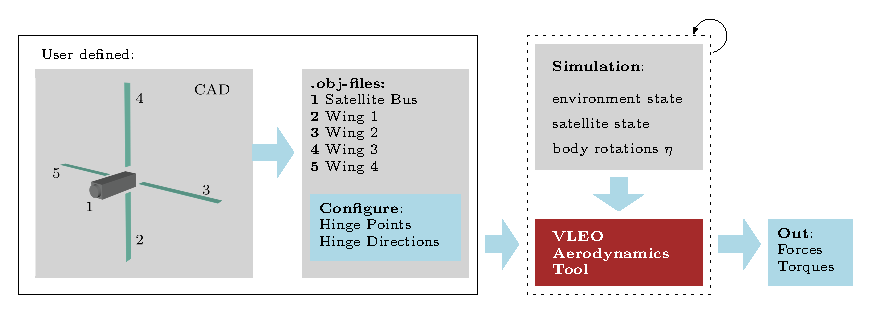
\includegraphics[width=0.9\textwidth]{Figures/fig8.eps}
		\caption{Aerodynamics tool workflow.}
			\label{fig:aerodynamics_tool_workflow}
	\end{figure}



    \section{Control Design}
	\label{sec:control_design}
	\subsection{Outer Loop Control}
	The satellite's attitude with respect to the tangential frame is given by the quaternion $q_{\text{BT}}$.
	We introduce the desired reference state $x_{\text{r}} = \begin{bmatrix}q_{\text{BT}}^{\text{r}} & \omega_{\text{BT,r}}^{\text{B}}\end{bmatrix}^{\top}$.
	Using the shorthand $q_{\text{BT}}=q$, we define the error quaternion with


	\newcommand{\tr}{\text{r}}
	\newcommand{\tO}{\text{}}
	\newcommand{\te}{\text{e}}
	\begin{equation}
		\label{eq:error_quaternion}
		q^{\te}
		= \begin{bmatrix}
			q_{\text{v}}^{\te} \\
			q_{4}^{\te}
		\end{bmatrix} 
		= \begin{bmatrix}
			q_{4}^{\tr} I - \tilde{q}_{\text{v}}^{\tr} & - q_{\text{v}}^{\tr} \\
			q_{\text{v}}^\intercal & q_{4}^{\tr}
		\end{bmatrix}
		q.
	\end{equation}
	Here, $I$ is the identity matrix and $\tilde{q}_{\text{v}}^{\tr}$ is the cross-product matrix of the vector part of the reference quaternion $q_{\text{v}}^{\tr}$. 
	The rate error is defined as $\omega_{\te} = \omega_{\text{BT,r}}^{\text{B}} - \omega_{\text{BT}}^{\text{B}}$.

	The desired torque can now be calculated using a PID version of the linear quaternion feedback regulator \cite{wieQuaternionFeedbackRegulator1989} with
	\begin{equation}
		\begin{aligned}
			\tau_{\text{des}} &= 
			- k_{\text{D}} J \omega_{\te}
			- k_{\text{P}} J q_{\text{v}}^{\te}
			- k_{\text{I}} \int_{0}^{t} q_{\text{v}}^{\te} \, \mathrm{d}\tau
		\end{aligned}
	\end{equation}

	where $k_{\text{D}}, k_{\text{P}}$ and $k_{\text{I}}$ are positive scalars.

	\subsection{Control Allocation}
	We now use \cref{eq:torque_simplified} and replace the panel normal vectors $\hat{n}_i$ with the control fin angles $\eta_i$. The generated aerodynamic torque can now be defined as a function of the incoming flow direction $\hat{v}_{\text{i}}$ given by the satellite's attitude (see \cref{eq:quat_to_flow}) and the commanded angles $\eta_i$. 
	This nonlinear function $\tau_{\text{aero}}(\eta,\hat{v}_{\text{i}})$ can be approximated by a linear function around the minimum-drag configuration to obtain

	\begin{equation}
		\Delta\tau_{\text{aero, lin}} = \tau_0 + A_0 \Delta \hat{v}_{\text{i}} + B_0\Delta \eta
	\end{equation}
	where
	\begin{align}
		A_0 &= \frac{\partial \tau_{\text{aero}}(\eta,\hat{v}_{\text{i}})}{\partial \hat{v}_{\text{i}}} \bigg|_{\eta = \eta_0, \hat{v}_{\text{i}} = \hat{v}_{\text{i}0}} \\
		B_0 &= \frac{\partial \tau_{\text{aero}}(\eta,\hat{v}_{\text{i}})}{\partial \eta} \bigg|_{\eta = \eta_0, \hat{v}_{\text{i}} = \hat{v}_{\text{i}0}}\\
		\eta_0 &= \mathbf{0}, \quad \tau_0 = \mathbf{0}, 
		\quad \hat{v}_{\text{i}0} = \begin{bmatrix}-1 & 0 & 0\end{bmatrix}^{\top}
	\end{align}
	around the stable equilibrium point. Since $\eta\in \mathbb{R}^4$ and $\hat{v}_{\text{i}} \in \mathbb{R}^3$, the matrix $B_0$ is of size $3\times 4$.
	We use the pseudoinverse to calculate the required fin angles $\eta$ for a desired torque $\tau_{\text{des}}$ with

	\begin{equation}
		\Delta \eta_{\text{alloc}} = B_0^+ (\tau_{\text{des}} - A_0 \Delta v_{\text{i}}).
	\end{equation}

	This results in a linear allocation procedure analogous to the controller derived in \cite{chenAerodynamicAttitudeControl2023}. Since the Taylor approximation is performed around the nominal satellite configuration, the resulting linearization is visualized by \Cref{fig:linearization} for each control fin. As a result, the algorithm treats drag as a constant value. Furthermore, values that are actually varying such as density $\rho$ and molecular speed ratio $s_{\text{i}}$ are assumed to be constant in this implementation.

    \section{Case Study}
	\label{sec:case_study}
	To analyze the performance of the linear allocation method, we consider a case study for aerodynamic attitude control in a simulation environment.

	
	\subsection{Simulation}
	\label{sec:simulation}
	The satellite's 6-DoF dynamics are integrated with the initial conditions for a circular orbit given in \Cref{tab:initial_conditions}. At the start of the simulation the angular velocity is zero with respect to the tangential frame $\omega_{\text{BT}}=[0,0,0]^{\top}$. While the quaternion representation is used for control purposes, Euler angles are used in this section to provide a more intuitive understanding of the satellite's attitude.
	The initial attitude is varied in yaw, pitch and roll with respect to the tangential frame using a 3-2-1 rotation sequence. For $\Phi=[\phi,\theta,\psi]^{\top}=[0,0,0]^{\top}$ the body frame is aligned with the tangential frame and the satellite is in the nominal orientation of lowest drag and behaves statically stable around the equilibrium without a control input $\eta=[0,0,0,0]^{\top}$.
	Environmental parameters are obtained using the NRLMSISE-00 model \cite{piconeNRLMSISE00EmpiricalModel2002} and used within the \textit{VLEO Aerodynamics Tool} introduced in \cref{sec:sim_tool}. 
	% The International Geomagnetic Reference Field (IGRF) \cite{alkenInternationalGeomagneticReference2021} model is used to calculate conrtributions of the magnetic field. 
	
	% table with 2 columns
	\begin{table}[ht]
		\centering
		\caption{Orbit used for the case study.}
		\begin{tabular}{l|l|l}
			\hline
			\textbf{Parameter} & \textbf{Symbol} & \textbf{Value} \\
			\hline
			Altitude & $h$ & $300\,\text{km}$ \\
			Orbit inclination & $i$ & $0^{\circ}$ \\
			Eccentricity & $e$ & $0$ \\
			\hline
		\end{tabular}
		\label{tab:initial_conditions}
	\end{table}

	The control parameters are set to $k_{\text{P}}=4.5 \times 10^{-4}$, $k_{\text{I}}=1\times 10^{-7}$ and $k_{\text{D}}=3\times 10^{-2}$. The simulation is run for $900\,\text{s}$.

	\subsection{Results}
	\label{sec:results}
	We compare the performance of the PID control law with linear allocation for two different initial conditions in a stabilization scenario, that is, $\Phi_{\text{ref}}=\omega_{\text{BT,r}}=\textbf{0}$. The first example considers a small initial attitude offset in pitch and yaw of 
	$[\phi, \theta, \psi]^{\top} = [0^{\circ}, -2^{\circ}, 3^{\circ}]^{\top}$. The results are visualized in \Cref{fig:small_angle_sim_results}. Stabilization is achieved in the tangential frame. However, offsets between desired body torques as computed by the outer loop PID control law and the actual aerodynamic torques are visible. For instance, the magnitude of the initial aerodynamic torque exceeds the desired torque by a factor of 1.9. For larger initial attitudes of $[\phi, \theta, \psi]^{\top} = [5^{\circ}, 10^{\circ}, -8^{\circ}]^{\top}$, this offset is even more pronounced, as shown in \Cref{fig:large_angle_sim_results}. Here, the aerodynamic torque around the $y_{\text{B}}$-axis exceeds the desired torque by a factor close to 4. 
	Consequently, the allocation procedure fails to accurately represent the aerodynamic torques, even for small initial offsets. In our analysis the reason for this is two-fold. First, the linearization of the aerodynamic model is only valid around the nominal configuration for lift, but not for drag. Second, the time-varying parameters such as density are not accounted for in the linear allocation scheme.
	Even though the actual and desired torques differ, the control law is able to stabilize the satellite in both cases. This can in part be attributed to the satellite being statically stable around the equilibrium point. Without the control fins however, asymptotic stability through damping would not be possible.

    % Sim results plot: small initial offsets
	\begin{figure*}[h]
		% This file was created by matlab2tikz.
%
%The latest updates can be retrieved from
%  http://www.mathworks.com/matlabcentral/fileexchange/22022-matlab2tikz-matlab2tikz
%where you can also make suggestions and rate matlab2tikz.
%
\definecolor{mycolor1}{rgb}{0.00000,0.44700,0.74100}%
\definecolor{mycolor2}{rgb}{0.85000,0.32500,0.09800}%
\definecolor{mycolor3}{rgb}{0.92900,0.69400,0.12500}%
\definecolor{mycolor4}{rgb}{0.49400,0.18400,0.55600}%
%
\begin{tikzpicture}

\begin{axis}[%
width=4.927cm,
height=2.93cm,
at={(0cm,4.07cm)},
scale only axis,
xmin=0,
xmax=900,
xlabel style={font=\color{white!15!black}},
xlabel={t (s)},
ymin=-3,
ymax=3,
ylabel style={font=\color{white!15!black}},
ylabel={$\text{Euler angles [}^\circ\text{]}$},
axis background/.style={fill=white},
axis x line*=bottom,
axis y line*=left,
xmajorgrids,
ymajorgrids,
legend style={legend cell align=left, align=left, draw=white!15!black}
]
\addplot [color=mycolor1, line width=1.2pt]
  table[row sep=crcr]{%
0	-0\\
7.79999999999995	3.8904520010874e-05\\
36.6	0.00197768728571646\\
48.3	-0.000382231174171466\\
61.3	-0.00522095494579844\\
78.4	-0.0138947475385294\\
118.5	-0.0349156538943589\\
135.3	-0.0411156792634984\\
151.3	-0.044895241458903\\
167.5	-0.0465758834860708\\
184.5	-0.0461789756190001\\
203	-0.0435677276875595\\
224	-0.0384044975135112\\
249.8	-0.0298211028429023\\
292.4	-0.0131466345642366\\
339.5	0.00461575604845166\\
370.8	0.0142515554856573\\
399.5	0.0209666100987533\\
427.7	0.0254260236865775\\
456.5	0.0278306187203725\\
487	0.0282180230973381\\
520.8	0.0264688581196424\\
561.2	0.0221524895451921\\
621.1	0.013356825320102\\
713.3	5.3434744131664e-06\\
766.7	-0.00542749012652166\\
818	-0.00849943579555656\\
872.5	-0.00958703910350778\\
900	-0.00942480286005321\\
};
\addlegendentry{$\phi$}

\addplot [color=mycolor2, line width=1.2pt]
  table[row sep=crcr]{%
0	-2\\
1.39999999999998	-2.00243355820282\\
2.79999999999995	-2.00270595673021\\
4.29999999999995	-2.00076035711004\\
5.79999999999995	-1.99666704430501\\
7.39999999999998	-1.99011580909075\\
9.10000000000002	-1.980886207911\\
10.8	-1.96952233106197\\
12.6	-1.95537809374116\\
14.5	-1.9383209298843\\
16.5	-1.91825268612195\\
18.7	-1.89395921059179\\
21	-1.8663844539808\\
23.5	-1.83423304530379\\
26.2	-1.79734588556209\\
29.2	-1.75417844981632\\
32.6	-1.70303814450699\\
36.5	-1.64218826034562\\
41.4	-1.56349315188436\\
49.2	-1.43574384412727\\
59.3	-1.27074750203508\\
65.3	-1.17492243000629\\
70.6	-1.09238496504793\\
75.6	-1.01666820695516\\
80.4	-0.946146074278204\\
85	-0.880677777412188\\
89.6	-0.817358085742285\\
94.1	-0.75753794308207\\
98.6	-0.699837257669969\\
103.1	-0.644257155507034\\
107.6	-0.59078427437214\\
112.2	-0.538275448995023\\
116.8	-0.48790740403922\\
121.5	-0.438611521378675\\
126.2	-0.39145613119706\\
131	-0.345450839085174\\
135.8	-0.301562513632007\\
140.7	-0.258880413175689\\
145.7	-0.217468857926633\\
150.8	-0.177386974666206\\
156	-0.138688957691102\\
161.3	-0.101424277076944\\
166.6	-0.0662809057366758\\
172	-0.032577965779069\\
177.6	0.000213384981975651\\
183.3	0.0314178166350985\\
189.1	0.0610092440463177\\
195	0.088966546765505\\
201	0.11527362183881\\
207.2	0.140306358174598\\
213.5	0.163605663640624\\
220	0.185494914524043\\
226.7	0.20588742465452\\
233.5	0.224450450715608\\
240.5	0.241438419580732\\
247.8	0.25699638929882\\
255.3	0.270828371832977\\
263.1	0.283052906856028\\
271.2	0.293580403751662\\
279.6	0.302341867632094\\
288.4	0.309357671499129\\
297.6	0.314533934626184\\
307.3	0.317830503078767\\
317.6	0.319157314218273\\
328.5	0.318405359589974\\
340.2	0.315449761447894\\
353	0.310041420948551\\
367.1	0.301899650326618\\
383	0.290526583343762\\
401.6	0.275013440631824\\
425.1	0.253156555843134\\
464.8	0.213713781809702\\
509.6	0.16987430119832\\
539.5	0.142782616785212\\
566.7	0.120256162472401\\
592.9	0.100684698697933\\
618.9	0.0833969353345765\\
645.2	0.0680527945896756\\
672.1	0.054500621736338\\
700	0.0425876351491752\\
729.3	0.0322254732477631\\
760.5	0.0233535640833225\\
794	0.0159894893524779\\
830.7	0.0100933917506154\\
871.6	0.00570115156892825\\
900	0.00373893757682708\\
};
\addlegendentry{$\theta$}

\addplot [color=mycolor3, line width=1.2pt]
  table[row sep=crcr]{%
0	3\\
1.20000000000005	2.99891307155463\\
2.39999999999998	2.99545369424766\\
3.70000000000005	2.98917870550429\\
5	2.98043725179514\\
6.39999999999998	2.96844827337839\\
7.79999999999995	2.95397525086582\\
9.29999999999995	2.93591869731051\\
10.8	2.91543215092952\\
12.4	2.89112745297348\\
14.1	2.8627803725642\\
15.9	2.83021078798447\\
17.8	2.79328526747076\\
19.8	2.75191803323048\\
22	2.70383120800295\\
24.3	2.65106967780014\\
26.9	2.58884541155101\\
29.7	2.51931730179047\\
32.9	2.43733006051912\\
36.7	2.33736981671973\\
41.5	2.20846599820845\\
51	1.95012822463298\\
58	1.76114276410544\\
63.2	1.62321170422433\\
67.8	1.50364135971006\\
72.1	1.39433710565856\\
76.2	1.29260006140998\\
80.2	1.19587050649011\\
84.1	1.10410111377485\\
87.9	1.01720061428398\\
91.6	0.935044949462849\\
95.3000000000001	0.855365622102227\\
99	0.77819715953899\\
102.7	0.703559859286315\\
106.4	0.631461486578701\\
110.1	0.561898781870923\\
113.8	0.494858881333698\\
117.5	0.430320601553831\\
121.2	0.368255621176672\\
124.9	0.308629526820027\\
128.7	0.249889003438511\\
132.5	0.19363175243268\\
136.4	0.138422310569126\\
140.3	0.0857155671311602\\
144.3	0.0341926929678493\\
148.3	-0.01483067315678\\
152.4	-0.0625585495055248\\
156.5	-0.107809945235203\\
160.7	-0.151677599984396\\
165	-0.194067347903456\\
169.3	-0.233992616783212\\
173.7	-0.272386418366978\\
178.2	-0.309174611033654\\
182.8	-0.3442904616752\\
187.5	-0.377674727181216\\
192.3	-0.409275678753261\\
197.2	-0.439049087974809\\
202.2	-0.466958161157663\\
207.4	-0.493459711505125\\
212.7	-0.517952835152755\\
218.1	-0.540427313114719\\
223.7	-0.561230039005295\\
229.5	-0.580237441091867\\
235.4	-0.597076726897967\\
241.5	-0.612001290691069\\
247.8	-0.624931345525738\\
254.4	-0.635951985246038\\
261.2	-0.644795997924916\\
268.3	-0.651516067493844\\
275.7	-0.656005520785129\\
283.4	-0.658185089291237\\
291.5	-0.657986545781341\\
300.1	-0.655257459848599\\
309.2	-0.649851630518015\\
318.9	-0.641579114796855\\
329.4	-0.63009396415157\\
340.8	-0.615096370484366\\
353.4	-0.595995310082003\\
367.7	-0.571780047521997\\
384.7	-0.54041626126434\\
407	-0.496612852211683\\
484.9	-0.34153228499531\\
507.5	-0.300217070389522\\
528.5	-0.264292612599206\\
548.8	-0.232045502469987\\
568.8	-0.202766184620486\\
588.7	-0.176118193494062\\
608.8	-0.151692587560547\\
629.3	-0.129285947798394\\
650.3	-0.108841438795707\\
672	-0.090228835828384\\
694.5	-0.0734355999693435\\
718.1	-0.058330118149911\\
743	-0.0449009290256299\\
769.6	-0.0330725160229122\\
798.3	-0.0228382128949534\\
829.6	-0.0142047582947953\\
864.4	-0.00714125945569322\\
900	-0.00210364007455155\\
};
\addlegendentry{$\psi$}

\end{axis}

\begin{axis}[%
width=4.927cm,
height=2.93cm,
at={(6.484cm,4.07cm)},
scale only axis,
xmin=0,
xmax=500,
xlabel style={font=\color{white!15!black}},
xlabel={t (s)},
ymin=-1.2e-06,
ymax=8e-07,
ylabel style={font=\color{white!15!black}},
ylabel={$\tau\text{ [Nm]}$},
axis background/.style={fill=white},
axis x line*=bottom,
axis y line*=left,
xmajorgrids,
ymajorgrids,
legend style={legend cell align=left, align=left, draw=white!15!black}
]
\addplot [color=mycolor1, line width=1.2pt]
  table[row sep=crcr]{%
0.899999999999977	-7.47849071558448e-09\\
5	-6.4443383962498e-09\\
9.69999999999999	-4.53388793175691e-09\\
15.8	-1.2859118214692e-09\\
29	5.91563775742543e-09\\
41	1.06851985037792e-08\\
59.4	1.50930645759217e-08\\
79.8	1.71534111359506e-08\\
91.8	1.7301488242083e-08\\
116.1	1.58855186782603e-08\\
130.2	1.44089540299319e-08\\
155.6	1.12985389932874e-08\\
197.4	6.41409769741585e-09\\
228.8	3.49160700352513e-09\\
261.1	1.20923004942597e-09\\
295.9	-5.27165866515134e-10\\
356.7	-2.1426558305393e-09\\
405.9	-2.50867060458404e-09\\
470.7	-2.23167262447532e-09\\
500.1	-1.9517756300047e-09\\
};
\addlegendentry{$\tau{}_{\text{A,x}}$}

\addplot [color=mycolor1, dashed, line width=1.2pt]
  table[row sep=crcr]{%
0	-5.92535798205063e-09\\
1.5	-5.63477442483418e-09\\
7.30000000000001	-3.95186816604109e-09\\
18.1	6.25846041657496e-11\\
30.1	4.2351189222245e-09\\
40.4	7.08485003997339e-09\\
50.9	9.27479959500488e-09\\
61.9	1.08472590909514e-08\\
73.6	1.1793247267633e-08\\
86.5	1.21058860713674e-08\\
101.6	1.17331069304782e-08\\
121.4	1.04844843917817e-08\\
164.1	6.85298573444015e-09\\
205.3	3.72904196410673e-09\\
243.3	1.57643853526679e-09\\
284.2	-1.60866875376087e-11\\
330.3	-1.08167341750232e-09\\
384.8	-1.60389390657656e-09\\
456.2	-1.53278278958169e-09\\
500.1	-1.26931354316184e-09\\
};
\addlegendentry{$\tau{}_{\text{des,x}}$}

\addplot [color=mycolor2, line width=1.2pt]
  table[row sep=crcr]{%
0.899999999999977	7.7250911090232e-07\\
1.69999999999999	7.42652446206193e-07\\
2.39999999999998	7.17149021056684e-07\\
3.39999999999998	6.8172465716998e-07\\
4.10000000000002	6.57642203805153e-07\\
4.89999999999998	6.30846841431776e-07\\
5.69999999999999	6.04828699124482e-07\\
6.5	5.79602215111663e-07\\
7.19999999999999	5.58165936581645e-07\\
8	5.3440027159013e-07\\
9.10000000000002	5.02991383655171e-07\\
10.2	4.73033082926122e-07\\
11	4.52140852758021e-07\\
11.8	4.31984176429978e-07\\
12.6	4.12586416587146e-07\\
13.2	3.98452868921595e-07\\
14	3.80248252440651e-07\\
14.8	3.62716548352182e-07\\
15.6	3.45833825576847e-07\\
16.5	3.27608006500668e-07\\
17.3	3.12040867811447e-07\\
18.2	2.95236930014653e-07\\
19.1	2.79132905234292e-07\\
20	2.63714753145905e-07\\
21	2.47346633841516e-07\\
22	2.31744024858926e-07\\
23	2.16869466385106e-07\\
24	2.02687488126685e-07\\
25.1	1.87846296739735e-07\\
26.2	1.7375833749611e-07\\
27.3	1.60383649472351e-07\\
28.4	1.47683522300213e-07\\
29.6	1.34555364184052e-07\\
31.4	1.16193746180215e-07\\
32.7	1.03857132671692e-07\\
34	9.22434537642403e-08\\
35.3	8.13085421214055e-08\\
36.7	7.02445959177567e-08\\
38.1	5.98945462115807e-08\\
39.1	5.28867190041638e-08\\
40.1	4.6175671286619e-08\\
41.7	3.60885792360932e-08\\
43.5	2.5612450826884e-08\\
45.2	1.64882294484414e-08\\
46.9	8.06267053121701e-09\\
48.7	-1.50976120494306e-10\\
50.5	-7.6892092693015e-09\\
53.6	-1.92276843336003e-08\\
55.7	-2.61001105172909e-08\\
57.9	-3.25597966366331e-08\\
60.2	-3.85782641387777e-08\\
63.1	-4.5171077545092e-08\\
67.1	-5.26841859027627e-08\\
69.2	-5.59734303351433e-08\\
73.8	-6.18121021034312e-08\\
77	-6.49134221930581e-08\\
80.3	-6.73831550557225e-08\\
83.9	-6.93710262567038e-08\\
87.8	-7.08071183908032e-08\\
92.1	-7.16690919944085e-08\\
96.9	-7.19069248589221e-08\\
102.4	-7.14489942765795e-08\\
108.9	-7.01722342455469e-08\\
114.1	-6.87584815750597e-08\\
119.3	-6.70875124342274e-08\\
122.8	-6.58729959468474e-08\\
130.6	-6.30203658147366e-08\\
169.2	-4.89091576127976e-08\\
190.2	-4.21501340497343e-08\\
213.3	-3.54121993950685e-08\\
237.9	-2.89506374429038e-08\\
262.7	-2.31439685194346e-08\\
287.3	-1.80909864866408e-08\\
312	-1.37269466904399e-08\\
337.1	-9.99784788291436e-09\\
363.6	-6.77226807965781e-09\\
367.5	-6.36634922557278e-09\\
395.8	-3.750983523787e-09\\
399.7	-3.45374928656383e-09\\
430.9	-1.40283873406588e-09\\
465.9	1.730313670123e-10\\
500.1	1.14226850200794e-09\\
};
\addlegendentry{$\tau{}_{\text{A,y}}$}

\addplot [color=mycolor2, dashed, line width=1.2pt]
  table[row sep=crcr]{%
0	3.07929440168664e-07\\
0.100000000000023	3.07456218706648e-07\\
1.10000000000002	2.85919441012084e-07\\
2	2.67344830717775e-07\\
2.89999999999998	2.49522884132602e-07\\
3.80000000000001	2.32433478686289e-07\\
4.69999999999999	2.16055013879668e-07\\
5.60000000000002	2.00366343960923e-07\\
6.5	1.85345299996698e-07\\
7.5	1.69411634942662e-07\\
8.5	1.54244673922221e-07\\
9.5	1.39813948862866e-07\\
10.5	1.26089389596018e-07\\
11.5	1.13040812266263e-07\\
12.6	9.94332367554307e-08\\
13.7	8.65700258145807e-08\\
14.8	7.44141743780347e-08\\
15.9	6.29303258392611e-08\\
17.1	5.11286089022178e-08\\
18.3	4.00437443204282e-08\\
19.5	2.96357711704331e-08\\
20.8	1.90806304090074e-08\\
22.1	9.23063225855003e-09\\
23.5	-6.36816821497632e-10\\
24.9	-9.78474190560519e-09\\
26.4	-1.88397279998753e-08\\
27.9	-2.71735416390584e-08\\
29.5	-3.53227846972004e-08\\
31.1	-4.27613713327446e-08\\
32.8	-4.99420593769173e-08\\
34.6	-5.67938513995614e-08\\
36.4	-6.29322016720835e-08\\
38.3	-6.86988528286747e-08\\
40.3	-7.40424752621038e-08\\
42.4	-7.89194700701046e-08\\
44.6	-8.32945374895644e-08\\
46.9	-8.71401653057546e-08\\
49.3	-9.04363446352363e-08\\
51.8	-9.31709678297921e-08\\
54.5	-9.54099732553004e-08\\
57.4	-9.70847509051964e-08\\
60.5	-9.81443122327619e-08\\
63.8	-9.85567680800159e-08\\
67.4	-9.82927303994074e-08\\
71.4	-9.72739258031652e-08\\
75.9	-9.53941139414383e-08\\
81.1	-9.24792402656749e-08\\
87.3	-8.82636186361196e-08\\
95.5	-8.19299543763918e-08\\
113.8	-6.68284201310598e-08\\
127.6	-5.58829924557358e-08\\
139.4	-4.72436454401759e-08\\
151	-3.94695121030963e-08\\
162.9	-3.22154960485932e-08\\
175.3	-2.53775169767323e-08\\
188.2	-1.89728552868473e-08\\
201.7	-1.29846284835367e-08\\
215.8	-7.44626049709041e-09\\
230.4	-2.42442865783232e-09\\
245.6	2.08922301681014e-09\\
261.4	6.06513594902935e-09\\
277.9	9.5016048362595e-09\\
295.3	1.24067014439788e-08\\
313.8	1.47731498145731e-08\\
333.6	1.65867959367461e-08\\
355.5	1.78592927113641e-08\\
379.7	1.85366957339284e-08\\
407.5	1.85890485226992e-08\\
441.5	1.79147718881723e-08\\
489.3	1.61810476129176e-08\\
500.1	1.57238559950201e-08\\
};
\addlegendentry{$\tau{}_{\text{des,y}}$}

\addplot [color=mycolor3, line width=1.2pt]
  table[row sep=crcr]{%
0.899999999999977	-1.1422894772295e-06\\
1.60000000000002	-1.1043088079532e-06\\
2.30000000000001	-1.06703276969711e-06\\
3	-1.03047653965405e-06\\
3.69999999999999	-9.9466353731259e-07\\
4.39999999999998	-9.59616613727121e-07\\
5.10000000000002	-9.25326332890108e-07\\
5.80000000000001	-8.91815545855934e-07\\
6.5	-8.59089198002039e-07\\
7.10000000000002	-8.31657587241352e-07\\
7.80000000000001	-8.00382963461743e-07\\
8.5	-7.69892494645319e-07\\
9.19999999999999	-7.40191296699777e-07\\
9.89999999999998	-7.11261463948176e-07\\
10.6	-6.83112546084885e-07\\
11.3	-6.55744997857255e-07\\
12.2	-6.21679589585256e-07\\
12.9	-5.96060829138878e-07\\
13.6	-5.71200587273779e-07\\
14.3	-5.47097499747906e-07\\
15	-5.23731330304145e-07\\
15.7	-5.01103045280615e-07\\
16.4	-4.79202753922436e-07\\
17.2	-4.55046290426253e-07\\
17.9	-4.34660989867552e-07\\
18.6	-4.14963324146811e-07\\
19.3	-3.95942834074958e-07\\
20	-3.77575531729235e-07\\
20.7	-3.59853686404676e-07\\
21.4	-3.42756663940236e-07\\
22.2	-3.23962808579381e-07\\
23	-3.05935259348189e-07\\
23.8	-2.88650653601508e-07\\
24.6	-2.72081308594352e-07\\
25.8	-2.48505273248156e-07\\
26.7	-2.31783189974522e-07\\
27.6	-2.15854242924252e-07\\
28.4	-2.02294472728681e-07\\
29.3	-1.87723060207645e-07\\
30.2	-1.73825981164555e-07\\
31.1	-1.60568731644162e-07\\
32.3	-1.43831186960597e-07\\
33.3	-1.30680973597919e-07\\
34	-1.21823177323677e-07\\
35.1	-1.08565643586189e-07\\
36.8	-8.94647769200674e-08\\
37.9	-7.79623405833263e-08\\
39.1	-6.60471641822369e-08\\
40.4	-5.39497477802797e-08\\
41.3	-4.59624516224721e-08\\
42.6	-3.50418076777714e-08\\
44	-2.39998598772218e-08\\
45.4	-1.36484459289932e-08\\
46.9	-3.26650706483633e-09\\
48.5	7.06086211721413e-09\\
50.1	1.66770064424782e-08\\
51.8	2.61754848907003e-08\\
53.6	3.5489165384206e-08\\
55.4	4.40984990746074e-08\\
57.3	5.24860297446139e-08\\
59.6	6.17401383351535e-08\\
61.7	6.94137725076871e-08\\
63.9	7.67254277889151e-08\\
66.1	8.33349531603744e-08\\
68.5	8.98246526048752e-08\\
71	9.58419832386426e-08\\
73.6	1.01360058124556e-07\\
76.3	1.06357276763447e-07\\
79	1.10667656372243e-07\\
83.7	1.16695218821405e-07\\
86.8	1.19740491300036e-07\\
88.9	1.21444429623807e-07\\
92.3	1.23600557344616e-07\\
95.9	1.25164774544828e-07\\
99.7	1.26103543607314e-07\\
103.8	1.26396002997353e-07\\
108.2	1.25991107324808e-07\\
113	1.24830648928764e-07\\
118.3	1.22841015581798e-07\\
131.7	1.15392992938723e-07\\
140.7	1.09208087906154e-07\\
157.6	9.65929416452127e-08\\
179	8.06948605713842e-08\\
200.9	6.5904600887734e-08\\
214	5.79724428462214e-08\\
227.3	5.06304331793217e-08\\
258.2	3.61575871465902e-08\\
273.1	3.03449496641406e-08\\
288.7	2.4977850898722e-08\\
305.1	2.00435010810907e-08\\
309.5	1.88460944627877e-08\\
327.2	1.44377736432943e-08\\
331.5	1.34808715301915e-08\\
350.5	9.65246726991609e-09\\
370.9	6.2597109717899e-09\\
393.1	3.28645910485648e-09\\
397.2	2.82602741208393e-09\\
399.8	2.532374310249e-09\\
424.5	1.77124093170278e-10\\
451.7	-1.70251723830006e-09\\
482.7	-3.12149950332241e-09\\
500.1	-3.64804009223008e-09\\
};
\addlegendentry{$\tau{}_{\text{A,z}}$}

\addplot [color=mycolor3, dashed, line width=1.2pt]
  table[row sep=crcr]{%
0	-4.61952765817841e-07\\
0.100000000000023	-4.61187369182881e-07\\
0.899999999999977	-4.35175309121405e-07\\
1.60000000000002	-4.13132568155561e-07\\
2.30000000000001	-3.91758987916546e-07\\
3	-3.71043711311358e-07\\
3.69999999999999	-3.50974573848362e-07\\
4.39999999999998	-3.31539411035919e-07\\
5.19999999999999	-3.10087898469646e-07\\
6	-2.89428555788618e-07\\
6.80000000000001	-2.6954211307384e-07\\
7.60000000000002	-2.50408618285292e-07\\
8.39999999999998	-2.32008119382954e-07\\
9.19999999999999	-2.14320493796549e-07\\
10	-1.97325732642639e-07\\
10.8	-1.81003372290434e-07\\
11.6	-1.65333460699912e-07\\
12.5	-1.484595486545e-07\\
13.4	-1.32357172333286e-07\\
14.3	-1.16997739496583e-07\\
15.2	-1.02352942121797e-07\\
16.1	-8.83944153429184e-08\\
17	-7.5094817475474e-08\\
18	-6.10570509707031e-08\\
19	-4.77621711070242e-08\\
20	-3.51745370608114e-08\\
21	-2.32593038163031e-08\\
22.1	-1.08894369077461e-08\\
23.2	7.50048911868362e-10\\
24.3	1.17002514343767e-08\\
25.5	2.29057377509889e-08\\
26.7	3.338476517456e-08\\
27.9	4.31826379099221e-08\\
29.2	5.30770876139286e-08\\
30.5	6.22712832409889e-08\\
31.9	7.14429120307614e-08\\
33.3	7.99093982095656e-08\\
34.8	8.82538984114944e-08\\
36.3	9.5900190899556e-08\\
37.9	1.03343325008609e-07\\
39.6	1.10505538941652e-07\\
41.3	1.16957892259961e-07\\
43.1	1.23076119962207e-07\\
45	1.28800309084909e-07\\
47	1.3407748156169e-07\\
49	1.38649966174853e-07\\
51.1	1.42755141041562e-07\\
53.3	1.46354693697504e-07\\
55.6	1.49416678141279e-07\\
58	1.51914150592347e-07\\
60.6	1.5388945939776e-07\\
63.3	1.55213456309866e-07\\
66.1	1.55881991759088e-07\\
69.1	1.55885743424733e-07\\
72.3	1.55167754201102e-07\\
75.7	1.53687096826616e-07\\
79.4	1.51347478549724e-07\\
83.4	1.48090066431905e-07\\
87.8	1.43780823691486e-07\\
92.7	1.38263033022668e-07\\
98.4	1.31120600599388e-07\\
105.5	1.21479956760595e-07\\
116.3	1.0601183930703e-07\\
133.8	8.09864104667213e-08\\
143.3	6.81566802995803e-08\\
152	5.71107534597104e-08\\
160.3	4.72769556836283e-08\\
168.5	3.82686948796618e-08\\
176.7	2.99663156511087e-08\\
185.1	2.21790514842723e-08\\
193.6	1.50116648001131e-08\\
202.4	8.30931412565405e-09\\
211.4	2.16573425859679e-09\\
220.8	-3.53486484527821e-09\\
230.6	-8.75763817020925e-09\\
240.8	-1.34767219606147e-08\\
251.5	-1.77115566657449e-08\\
262.8	-2.14647002394486e-08\\
274.7	-2.47015350396396e-08\\
287.4	-2.74378066933423e-08\\
301	-2.96470261673676e-08\\
315.7	-3.13103782900725e-08\\
331.7	-3.23947801916802e-08\\
349.3	-3.28627720591612e-08\\
369.1	-3.26613758261374e-08\\
391.9	-3.16983346237976e-08\\
419.5	-2.97923179459758e-08\\
456.4	-2.6483519377507e-08\\
500.1	-2.21061782212928e-08\\
};
\addlegendentry{$\tau{}_{\text{des,z}}$}

\end{axis}

\begin{axis}[%
width=4.927cm,
height=2.93cm,
at={(0cm,0cm)},
scale only axis,
xmin=0,
xmax=900,
xlabel style={font=\color{white!15!black}},
xlabel={t (s)},
ymin=-15,
ymax=15,
ylabel style={font=\color{white!15!black}},
ylabel={$\text{Fin angle [}^\circ\text{]}$},
axis background/.style={fill=white},
axis x line*=bottom,
axis y line*=left,
xmajorgrids,
ymajorgrids,
legend style={legend cell align=left, align=left, draw=white!15!black}
]
\addplot [color=mycolor1, line width=1.2pt]
  table[row sep=crcr]{%
0	0\\
0.100000000000023	12.1003898743727\\
0.200000000000045	12.0804102503211\\
0.899999999999977	11.48376013683\\
1.5	10.9861831432311\\
2.10000000000002	10.5014659210585\\
2.70000000000005	10.0294294979324\\
3.29999999999995	9.56989083856615\\
3.89999999999998	9.12265091113079\\
4.5	8.68750909596383\\
5.10000000000002	8.2642609084935\\
5.70000000000005	7.85269656137336\\
6.29999999999995	7.45260199145514\\
6.89999999999998	7.0637683358807\\
7.5	6.68597639420364\\
8.20000000000005	6.25888494077651\\
8.89999999999998	5.84617873911861\\
9.60000000000002	5.4475061616904\\
10.3	5.06252140710592\\
11	4.69087321479947\\
11.7	4.33220785713945\\
12.4	3.98618132163176\\
13.1	3.65244311296442\\
13.8	3.33063828010711\\
14.5	3.02042223786157\\
15.2	2.72145227458384\\
15.9	2.43337643053485\\
16.6	2.15586598542529\\
17.3	1.88857786827089\\
18.1	1.59520049787307\\
18.9	1.31425416778484\\
19.7	1.04526432317641\\
20.5	0.787761305613117\\
21.3	0.541291644820717\\
22.1	0.30541411723857\\
22.9	0.0796981247519852\\
23.8	-0.162602718307767\\
24.7	-0.393140255550179\\
25.6	-0.612460506177513\\
26.5	-0.821078531245803\\
27.4	-1.01950118394848\\
28.4	-1.22858656873927\\
29.4	-1.42628876644358\\
30.4	-1.6131888975159\\
31.4	-1.78984427035061\\
32.5	-1.97294756163456\\
33.6	-2.14493087405174\\
34.7	-2.30639449895557\\
35.9	-2.47121632824678\\
37.1	-2.62488506231045\\
38.3	-2.76803470550908\\
39.6	-2.91192743703584\\
40.9	-3.04487258079735\\
42.2	-3.16751026734551\\
43.6	-3.28873226296571\\
45	-3.39937663140483\\
46.5	-3.50690504957993\\
48	-3.60373558412198\\
49.6	-3.69597713473127\\
51.2	-3.77753422403748\\
52.9	-3.85324096065369\\
54.6	-3.91840721498613\\
56.4	-3.9766850391062\\
58.3	-4.0270479477889\\
60.2	-4.06676770164393\\
62.2	-4.0979090243801\\
64.3	-4.11970401624274\\
66.5	-4.13149669432653\\
68.8	-4.13273523728344\\
71.2	-4.12297381271731\\
73.7	-4.10189489189145\\
76.3	-4.06930269984264\\
79.1	-4.0232992458275\\
82.1	-3.96287697102548\\
85.3000000000001	-3.88732875315895\\
88.7	-3.79625929731071\\
92.5	-3.68342230558278\\
96.7	-3.54767888232902\\
101.5	-3.38162705804905\\
107.4	-3.1663669555835\\
116	-2.84071555256924\\
131.6	-2.24928388920193\\
139.3	-1.96917351599836\\
146.1	-1.73226303361901\\
152.6	-1.51631875960618\\
158.9	-1.31764572695852\\
165.1	-1.13272476845111\\
171.3	-0.958439868216374\\
177.5	-0.794736557933788\\
183.8	-0.63904874397906\\
190.2	-0.491599649827208\\
196.7	-0.352520009213549\\
203.4	-0.219961270758063\\
210.2	-0.0961224270271259\\
217.2	0.0206716899481307\\
224.4	0.13011519736699\\
231.9	0.23328152588374\\
239.6	0.328422115356375\\
247.6	0.416484627371915\\
255.9	0.497069830659257\\
264.5	0.569861091237158\\
273.5	0.635311027003695\\
282.9	0.69296097530173\\
292.8	0.742928923762747\\
303.2	0.78471199123419\\
314.3	0.818485022810819\\
326.1	0.843548828445705\\
338.7	0.859532511281259\\
352.4	0.866054649545617\\
367.3	0.862335921673889\\
384.1	0.847075899903984\\
403.2	0.818540373961241\\
425.5	0.774158111413726\\
454.6	0.704638433939863\\
504.3	0.573093900229196\\
558.7	0.432330242536295\\
597.8	0.341834593328826\\
634.2	0.268291315048259\\
669.2	0.207901769745149\\
706	0.155069974583057\\
744.6	0.110523691788785\\
786	0.0736292823972917\\
831.6	0.0439227244216909\\
883.5	0.0211238276032191\\
900	0.0158355300202402\\
};
\addlegendentry{$\eta{}_{\text{1}}$}

\addplot [color=mycolor2, line width=1.2pt]
  table[row sep=crcr]{%
0	0\\
0.100000000000023	-8.01545365144966\\
0.200000000000045	-8.00306954155747\\
1	-7.55174666714743\\
1.70000000000005	-7.16988036520684\\
2.39999999999998	-6.80012023021379\\
3.10000000000002	-6.44221346616735\\
3.79999999999995	-6.09590051560713\\
4.5	-5.76091515563746\\
5.20000000000005	-5.43699018357199\\
5.89999999999998	-5.12385730448932\\
6.60000000000002	-4.82123776574861\\
7.39999999999998	-4.48791439003446\\
8.20000000000005	-4.16755509790858\\
9	-3.85974482142819\\
9.79999999999995	-3.56407245963965\\
10.6	-3.28013627980613\\
11.4	-3.00752592872004\\
12.2	-2.74584030277811\\
13	-2.49469254726739\\
13.8	-2.2537018068499\\
14.7	-1.99425806008787\\
15.6	-1.74668005421972\\
16.5	-1.51046876675866\\
17.4	-1.28514231932581\\
18.3	-1.07024139095154\\
19.3	-0.843152189821126\\
20.3	-0.627804901158811\\
21.3	-0.423653593097015\\
22.3	-0.230173004075368\\
23.3	-0.0468641620733479\\
24.4	0.143589179243918\\
25.5	0.322904724260752\\
26.6	0.491647394197344\\
27.8	0.664287579251209\\
29	0.825628557796222\\
30.2	0.976285179175079\\
31.5	1.12809791490827\\
32.8	1.26873196253905\\
34.1	1.39883091630645\\
35.5	1.52784898902303\\
36.9	1.64606001418895\\
38.4	1.76147511783165\\
39.9	1.8659998226849\\
41.5	1.96628810677123\\
43.1	2.05579044486603\\
44.8	2.1399070315083\\
46.5	2.21352854727104\\
48.3	2.2808930851653\\
50.2	2.3411034188091\\
52.2	2.39339601644633\\
54.3	2.43713187615049\\
56.5	2.47181132456387\\
58.8	2.49708280591415\\
61.2	2.51271784020798\\
63.8	2.51867147521671\\
66.5	2.51422268719591\\
69.5	2.49826189752071\\
72.7	2.4703447378339\\
76.2	2.42908290659841\\
80.2	2.37084040848981\\
84.8000000000001	2.29262273084134\\
90.3000000000001	2.18789873247715\\
97.7	2.03543679484198\\
125.8	1.44638699442373\\
134.7	1.27587357162395\\
143.4	1.1198201340959\\
152.2	0.97269518979067\\
161.2	0.832925770366387\\
170.5	0.699163074163039\\
180.2	0.57032311185651\\
190.2	0.448124462079591\\
200.6	0.331744797534043\\
211.3	0.222654508992264\\
222.4	0.12019603826468\\
233.8	0.0256723438047857\\
245.5	-0.060701450495344\\
257.6	-0.13934814013669\\
270.1	-0.209898270375675\\
283.1	-0.272527809905455\\
296.6	-0.326861269304004\\
310.8	-0.373260737023315\\
325.9	-0.411713133057901\\
341.9	-0.441620055156591\\
359.1	-0.462977661377408\\
377.9	-0.475534259088931\\
398.9	-0.478709023060333\\
423.1	-0.471410765057271\\
452.4	-0.451477371689407\\
492.2	-0.412959389433013\\
642.4	-0.258534839648746\\
697	-0.218469962535096\\
754.5	-0.187199054275993\\
816.3	-0.163861508896957\\
896.4	-0.144647619410534\\
900	-0.143987812552609\\
};
\addlegendentry{$\eta{}_{\text{2}}$}

\addplot [color=mycolor3, line width=1.2pt]
  table[row sep=crcr]{%
0	0\\
0.100000000000023	-12.0398481514817\\
0.200000000000045	-12.0198297122261\\
0.899999999999977	-11.424614502048\\
1.5	-10.9283773756576\\
2.10000000000002	-10.4450965245941\\
2.70000000000005	-9.97458520961777\\
3.29999999999995	-9.51665664018776\\
3.89999999999998	-9.07110590386185\\
4.5	-8.63772715546315\\
5.10000000000002	-8.21631080979648\\
5.70000000000005	-7.80664239091686\\
6.29999999999995	-7.4085027378818\\
6.89999999999998	-7.02167811223683\\
7.5	-6.64594475365152\\
8.10000000000002	-6.28108117107104\\
8.79999999999995	-5.86884616020632\\
9.5	-5.47074357343752\\
10.2	-5.0864238714837\\
10.9	-4.71552152172978\\
11.6	-4.35768715950371\\
12.3	-4.01256059535569\\
13	-3.67979309492102\\
13.7	-3.35902304723356\\
14.4	-3.0499004534164\\
15.1	-2.75207663062827\\
15.8	-2.46519697494318\\
16.5	-2.1889268572321\\
17.2	-1.92291968257791\\
18	-1.63105069052517\\
18.8	-1.35165524045169\\
19.6	-1.08425299657517\\
20.4	-0.8283701419316\\
21.2	-0.583548204680824\\
22	-0.349341680753923\\
22.8	-0.125316119016134\\
23.7	0.115064125023878\\
24.6	0.343663652683404\\
25.5	0.561037754082463\\
26.4	0.767706695294237\\
27.3	0.964175161109665\\
28.3	1.1710913328543\\
29.3	1.3666306090422\\
30.3	1.55137920110985\\
31.3	1.72589516264088\\
32.4	1.90666910890434\\
33.5	2.07634721611191\\
34.6	2.23553592589462\\
35.8	2.3979132873792\\
37	2.54918075280136\\
38.2	2.68997701617036\\
39.5	2.8313769339436\\
40.8	2.96189138670366\\
42.1	3.08216193685723\\
43.5	3.20091503224342\\
44.9	3.30917114785007\\
46.4	3.41423450045193\\
47.9	3.5086996980823\\
49.5	3.59852990911929\\
51.1	3.67779357824236\\
52.8	3.75119435180704\\
54.5	3.81418845145186\\
56.3	3.87031775652088\\
58.2	3.91857824697297\\
60.1	3.95636525925261\\
62.1	3.9856547277783\\
64.2	4.00570515947504\\
66.4	4.0158856158514\\
68.7	4.01566983079306\\
71.1	4.00463777551431\\
73.6	3.98249513934627\\
76.3	3.94758567791098\\
79.1	3.90060932056008\\
82.1	3.83951768342547\\
85.3000000000001	3.76365455550706\\
88.8000000000001	3.66985059405397\\
92.6	3.55731326212037\\
96.9	3.41916144798506\\
101.9	3.24757842832344\\
108.2	3.02008176315337\\
118.5	2.63561837158079\\
130.7	2.18315475903012\\
138.4	1.90844914231536\\
145.3	1.67284660145208\\
151.9	1.45822141692668\\
158.2	1.26394060890846\\
164.5	1.08039517416728\\
170.7	0.910355837621978\\
177	0.748272686855557\\
183.3	0.596776276449191\\
189.8	0.451264383728585\\
196.4	0.314331629821822\\
203.1	0.186004152460896\\
210	0.0645626123268812\\
217.1	-0.0496385981844014\\
224.4	-0.156324890270298\\
232	-0.256545579294198\\
239.8	-0.34864380303884\\
247.9	-0.433547850422201\\
256.3	-0.510898514479095\\
265.1	-0.581158743381025\\
274.3	-0.643806863284453\\
283.9	-0.698452153058611\\
294	-0.745240627518456\\
304.7	-0.784059757124624\\
316.1	-0.814593049987479\\
328.3	-0.836398423674837\\
341.4	-0.848958315304799\\
355.6	-0.851776496066464\\
371.3	-0.844010259037987\\
388.9	-0.824370357166913\\
409.2	-0.790728406296353\\
433.8	-0.738851990431385\\
468.3	-0.654182012301703\\
573.5	-0.389309713423245\\
611.7	-0.307644638029842\\
648.4	-0.239886676781566\\
685.4	-0.182355602126336\\
723.7	-0.133600885496776\\
764.4	-0.0926498501647757\\
808.7	-0.0589974936754061\\
858.2	-0.032375420182575\\
900	-0.0169736154063003\\
};
\addlegendentry{$\eta{}_{\text{3}}$}

\addplot [color=mycolor4, line width=1.2pt]
  table[row sep=crcr]{%
0	0\\
0.100000000000023	8.07599537434066\\
0.200000000000045	8.06365007965246\\
1	7.61067576836433\\
1.70000000000005	7.22721780033316\\
2.39999999999998	6.85573808261711\\
3.10000000000002	6.49599351164375\\
3.79999999999995	6.1477323739299\\
4.5	5.81069709613814\\
5.20000000000005	5.48462859115318\\
5.89999999999998	5.16926580539496\\
6.60000000000002	4.86433898399389\\
7.39999999999998	4.52829237638355\\
8.20000000000005	4.20512843568849\\
9	3.89444277141274\\
9.79999999999995	3.59583391385866\\
10.6	3.30890883702205\\
11.4	3.03326797709371\\
12.2	2.76851768173753\\
13	2.51428052099777\\
13.8	2.27018188464706\\
14.7	2.00722961644988\\
15.6	1.75613892277227\\
16.5	1.51641854816694\\
17.4	1.28759544246861\\
18.3	1.06921678475499\\
19.3	0.838292573952799\\
20.3	0.619148767329875\\
21.3	0.411244279931225\\
22.3	0.214060000881318\\
23.3	0.0271009679296412\\
24.4	-0.167301795735511\\
25.5	-0.350494181815861\\
26.6	-0.523037152616325\\
27.7	-0.685454122788883\\
28.9	-0.851681609869843\\
30.1	-1.00707841640769\\
31.3	-1.15221517735699\\
32.6	-1.29850357151702\\
33.9	-1.43404482885205\\
35.3	-1.56869322870034\\
36.7	-1.69230123228533\\
38.1	-1.80553719588841\\
39.6	-1.91606389791355\\
41.1	-2.01611876526999\\
42.7	-2.11205857168511\\
44.3	-2.19760996467301\\
46	-2.27791959514627\\
47.8	-2.35192472634037\\
49.6	-2.41543318296522\\
51.5	-2.47197812667594\\
53.5	-2.52080746894831\\
55.6	-2.56129246261787\\
57.8	-2.59294528074008\\
60.1	-2.61539934003156\\
62.6	-2.62875915515542\\
65.2	-2.6318195543198\\
68	-2.62426215448806\\
71	-2.60535053200044\\
74.3	-2.57355207453145\\
77.9	-2.52793595234891\\
81.9	-2.46648181040473\\
86.6	-2.38316086653163\\
92.2	-2.27279436889205\\
99.8000000000001	-2.11155667272863\\
127.2	-1.52137151176862\\
136.3	-1.34108644697017\\
145.1	-1.17746705898628\\
153.9	-1.02453396285534\\
162.9	-0.878830324029082\\
172.2	-0.739055184379936\\
181.9	-0.60415060269338\\
191.8	-0.477271451593765\\
202	-0.357296776270118\\
212.5	-0.244506020466588\\
223.3	-0.139195104206919\\
234.5	-0.0408316901407488\\
246	0.0493043910179267\\
257.8	0.130990654674065\\
269.9	0.204078289879476\\
282.5	0.269457043922898\\
295.6	0.326681174824785\\
309.3	0.37577298866222\\
323.7	0.416646481081102\\
339	0.449328639602641\\
355.4	0.473584558545213\\
373.2	0.489125963465995\\
392.9	0.495478648039352\\
415.6	0.49159075057139\\
441.9	0.475997653813124\\
475.4	0.444910344438085\\
530.8	0.381181864103382\\
610.2	0.292080743848942\\
663.2	0.243953290021864\\
715.8	0.207040079611033\\
772.3	0.178333441104087\\
837.5	0.156314391926685\\
900	0.142849727166549\\
};
\addlegendentry{$\eta{}_{\text{4}}$}

\end{axis}

\begin{axis}[%
width=4.927cm,
height=2.93cm,
at={(6.484cm,0cm)},
scale only axis,
xmin=0,
xmax=900,
xlabel style={font=\color{white!15!black}},
xlabel={t (s)},
ymin=-0.03,
ymax=0.02,
ylabel style={font=\color{white!15!black}},
ylabel={$\text{angular velocity [}^\circ\text{/s]}$},
axis background/.style={fill=white},
axis x line*=bottom,
axis y line*=left,
xmajorgrids,
ymajorgrids,
legend style={legend cell align=left, align=left, draw=white!15!black}
]
\addplot [color=mycolor1, line width=1.2pt]
  table[row sep=crcr]{%
0	-0\\
0.600000000000023	-7.81650282988267e-06\\
4	-7.12917852752071e-05\\
8.39999999999998	-0.000172178573166093\\
25.3	-0.000577045232830642\\
30.7	-0.000678927967442178\\
36.1	-0.000763148481837561\\
41.6	-0.000831292106568071\\
47.3	-0.000884141178403297\\
53.2	-0.000921029388678107\\
59.4	-0.000941750803917785\\
65.9	-0.000945402542129159\\
72.8	-0.000931292706354725\\
80.3000000000001	-0.000897871282404594\\
88.7	-0.000842117562683597\\
98.5	-0.000758583335937146\\
111.2	-0.000631321295486487\\
160.3	-0.000121710056077973\\
174.8	9.3877326889924e-07\\
188.9	0.000102377985967905\\
203	0.000186022405500808\\
217.5	0.000254160472081821\\
232.6	0.000307136761080073\\
248.5	0.000344895243642895\\
265.4	0.00036705732190967\\
283.7	0.000373078025063478\\
304	0.000361624365837088\\
327.2	0.00033027551808118\\
355.5	0.000273514669629549\\
398.1	0.000168132100839102\\
465.2	3.59635487257037e-06\\
502.4	-6.84686503973353e-05\\
536.9	-0.000117517319949911\\
571.2	-0.000148392941127895\\
607	-0.000162628071279869\\
646.3	-0.000160082614911516\\
692.8	-0.000138570153808359\\
760.4	-8.74965919592796e-05\\
876.9	4.24471295445983e-07\\
900	1.30195497831664e-05\\
};
\addlegendentry{$\omega{}_{\text{e,1}}$}

\addplot [color=mycolor2, line width=1.2pt]
  table[row sep=crcr]{%
0	0\\
0.100000000000023	3.33954084226207e-05\\
0.700000000000045	0.000728857021272233\\
1.29999999999995	0.00140477349873436\\
1.89999999999998	0.00206106341806844\\
2.5	0.00269810563452211\\
3.10000000000002	0.00331626024944853\\
3.70000000000005	0.00391590462970726\\
4.29999999999995	0.00449742094474459\\
4.89999999999998	0.00506119006070094\\
5.5	0.00560759149084333\\
6.10000000000002	0.00613701585348281\\
6.70000000000005	0.00664984213517528\\
7.29999999999995	0.00714645856476182\\
7.89999999999998	0.00762724996241104\\
8.5	0.00809260491428176\\
9.20000000000005	0.00861651037041611\\
9.89999999999998	0.00912052094213323\\
10.6	0.00960522707396194\\
11.3	0.0100712225156485\\
12	0.0105190919393863\\
12.7	0.0109493950321848\\
13.4	0.0113626865138485\\
14.1	0.0117595157012147\\
14.8	0.0121404190975909\\
15.6	0.012556888780523\\
16.4	0.012953977002212\\
17.2	0.0133324101038852\\
18	0.0136928862059449\\
18.8	0.0140360818368208\\
19.6	0.0143626492846352\\
20.5	0.0147109366573659\\
21.4	0.0150398224395758\\
22.3	0.0153501180221838\\
23.2	0.0156426048656613\\
24.1	0.0159180336216878\\
25	0.0161771202135697\\
26	0.0164466533049108\\
27	0.0166977397218488\\
28	0.016931223595634\\
29	0.0171479176678986\\
30.1	0.0173678087704729\\
31.2	0.0175692725439376\\
32.3	0.017753234232373\\
33.4	0.0179205649610594\\
34.6	0.0180851099727306\\
35.8	0.0182318589074839\\
37	0.0183617657166906\\
38.3	0.0184845549262036\\
39.6	0.0185897255710188\\
41	0.0186844618531268\\
42.4	0.018761156858659\\
43.9	0.0188245944417531\\
45.4	0.0188699279133289\\
47	0.0188997055846585\\
48.6	0.0189116541004068\\
50.3	0.0189062656172609\\
52.1	0.0188818343384582\\
53.9	0.0188397105903277\\
55.8	0.018777696470579\\
57.8	0.0186947114203804\\
59.9	0.0185899060855945\\
62.1	0.0184627007128029\\
64.5	0.0183059087379434\\
67.1	0.0181174461368983\\
69.9	0.0178958757634291\\
72.9	0.017640414827838\\
76.3	0.017332380880589\\
80.1	0.0169698073764266\\
84.6	0.0165221680474588\\
90.5	0.0159162768835586\\
113.8	0.0135048429153812\\
120.1	0.0128808655068724\\
126.1	0.0123045378587676\\
131.9	0.0117653528164965\\
137.6	0.0112532391530067\\
143.3	0.0107589227770859\\
149	0.0102823431037677\\
154.8	0.00981534612674295\\
160.6	0.00936607507151166\\
166.5	0.00892679896287518\\
172.5	0.00849794934617876\\
178.6	0.00807982163075849\\
184.8	0.00767285358210756\\
191	0.00728358404319351\\
197.3	0.00690566830621719\\
203.7	0.00653944869168299\\
210.2	0.006185256648223\\
216.8	0.00584340794671334\\
223.5	0.0055142096327927\\
230.3	0.00519794677325081\\
237.2	0.0048948613077755\\
244.2	0.00460515989288979\\
251.3	0.00432903596163214\\
258.6	0.00406310361256601\\
266	0.00381144880691409\\
273.5	0.00357408266995662\\
281.2	0.00334816909560232\\
289.1	0.00313429270761389\\
297.2	0.00293295249116454\\
305.5	0.00274455080784719\\
314	0.00256938954112229\\
322.8	0.00240591512283572\\
331.9	0.0022548133190412\\
341.3	0.0021166149781493\\
351.1	0.00199051100094039\\
361.3	0.00187725184241572\\
371.9	0.00177736352725333\\
383.2	0.00168905034422551\\
395	0.00161488470098448\\
407.5	0.00155422559089402\\
420.9	0.00150721677357524\\
435.3	0.00147468370369097\\
451	0.0014572404794535\\
468.4	0.00145605392640391\\
488.3	0.00147326924673052\\
511.2	0.0015114703207928\\
539.7	0.00157762922083293\\
581.5	0.00169425744877572\\
672.6	0.00195144936924407\\
717.4	0.00205710918567092\\
760.2	0.00214013614845499\\
802.2	0.00220446862704193\\
847.9	0.0022566356066136\\
895.3	0.00229368170425914\\
900	0.00229651934807862\\
};
\addlegendentry{$\omega{}_{\text{e,2}}$}

\addplot [color=mycolor3, line width=1.2pt]
  table[row sep=crcr]{%
0	-0\\
0.100000000000023	-5.00249984725087e-05\\
0.600000000000023	-0.000908937482336114\\
1.10000000000002	-0.00174827271587219\\
1.60000000000002	-0.00256765161452677\\
2.10000000000002	-0.0033673327999395\\
2.60000000000002	-0.00414757888370332\\
3.10000000000002	-0.00490865134111118\\
3.60000000000002	-0.00565083436447367\\
4.10000000000002	-0.00637440628474906\\
4.60000000000002	-0.00707965289018375\\
5.10000000000002	-0.00776685816447298\\
5.60000000000002	-0.0084363134465093\\
6.10000000000002	-0.0090883127924144\\
6.60000000000002	-0.00972313833665339\\
7.10000000000002	-0.0103410863358704\\
7.60000000000002	-0.0109424512869509\\
8.10000000000002	-0.0115275245918838\\
8.60000000000002	-0.0120966010872507\\
9.10000000000002	-0.0126499764897972\\
9.60000000000002	-0.0131879340143541\\
10.1	-0.0137107685629871\\
10.7	-0.0143186291280699\\
11.3	-0.0149056233706233\\
11.9	-0.0154722761968742\\
12.5	-0.0160190527063833\\
13.1	-0.0165464616262625\\
13.7	-0.0170549991174767\\
14.3	-0.0175451465203196\\
14.9	-0.0180173823389396\\
15.5	-0.0184721898366433\\
16.1	-0.0189100509811624\\
16.7	-0.0193314182280346\\
17.3	-0.0197367570427787\\
17.9	-0.0201265254326017\\
18.6	-0.0205621765535398\\
19.3	-0.0209779399671106\\
20	-0.0213745028120229\\
20.7	-0.0217525371608644\\
21.4	-0.0221126843456432\\
22.1	-0.0224555825698189\\
22.8	-0.0227818488253888\\
23.5	-0.0230920805855703\\
24.3	-0.0234277389633917\\
25.1	-0.0237440539261797\\
25.9	-0.0240418144854857\\
26.7	-0.0243217940180784\\
27.5	-0.0245847336491352\\
28.3	-0.0248313411894969\\
29.2	-0.0250900971000192\\
30.1	-0.0253299548862742\\
31	-0.0255517938431922\\
31.9	-0.025756445495972\\
32.8	-0.0259446836449797\\
33.8	-0.0261355077577718\\
34.8	-0.0263079574173162\\
35.8	-0.0264629496758744\\
36.8	-0.0266013415402995\\
37.9	-0.0267353434613824\\
39	-0.0268512458962959\\
40.1	-0.0269499832018028\\
41.3	-0.0270391648290342\\
42.5	-0.0271100577717789\\
43.7	-0.02716365672336\\
45	-0.0272033028563783\\
46.3	-0.0272248781495819\\
47.6	-0.027229423345716\\
49	-0.0272163868685311\\
50.4	-0.0271858577343664\\
51.9	-0.0271349234262743\\
53.4	-0.0270663240020212\\
55	-0.0269749559630554\\
56.6	-0.0268660340321958\\
58.3	-0.0267324035112324\\
60.1	-0.0265722543313132\\
61.9	-0.0263943491715963\\
63.8	-0.026188800864702\\
65.8	-0.0259543468739594\\
67.9	-0.0256899507662638\\
70.1	-0.0253948047954964\\
72.4	-0.0250683683646002\\
74.9	-0.024695095332504\\
77.5	-0.0242889601983052\\
80.3000000000001	-0.023833885949557\\
83.4	-0.0233119262190939\\
86.8000000000001	-0.0227215211923522\\
90.7	-0.0220263463347692\\
95.5	-0.021152239873004\\
102.7	-0.0198210008034039\\
113.4	-0.0178442856122274\\
119.1	-0.0168101436038341\\
124.1	-0.0159208056426223\\
128.7	-0.0151203804192619\\
133.1	-0.0143726432456788\\
137.3	-0.0136765055959813\\
141.4	-0.0130144321780108\\
145.5	-0.0123702700095691\\
149.5	-0.0117594329817621\\
153.5	-0.011166289190669\\
157.5	-0.0105910080937974\\
161.5	-0.0100336131202994\\
165.5	-0.0094940390845295\\
169.5	-0.00897214308906769\\
173.5	-0.00846772674822205\\
177.6	-0.00796857969032772\\
181.7	-0.00748722767025356\\
185.9	-0.0070122329689184\\
190.1	-0.0065551592489328\\
194.3	-0.00611559090839364\\
198.6	-0.00568323379229696\\
203	-0.00525885721060604\\
207.4	-0.00485220662653774\\
211.9	-0.00445411190503364\\
216.5	-0.00406520949445621\\
221.1	-0.00369395021255059\\
225.8	-0.00333226465454572\\
230.6	-0.00298063222612654\\
235.5	-0.00263954611250483\\
240.5	-0.00230942973416859\\
245.6	-0.00199065505501039\\
250.8	-0.00168356314100038\\
256.1	-0.00138845097706053\\
261.5	-0.00110557675679956\\
267	-0.000835148842156741\\
272.7	-0.000572883954987446\\
278.5	-0.000323965121879155\\
284.4	-8.84543188703901e-05\\
290.5	0.000137191741941933\\
296.8	0.000352155435734858\\
303.2	0.000552709642647642\\
309.8	0.000741750674706054\\
316.6	0.000918708635822441\\
323.7	0.00108533611557959\\
331	0.00123854369451237\\
338.5	0.00137807758824238\\
346.3	0.00150529486484174\\
354.4	0.00161950999859073\\
362.8	0.00172014870508974\\
371.6	0.00180771912050659\\
380.8	0.00188141591911517\\
390.5	0.00194119718787533\\
400.7	0.00198619308457637\\
411.6	0.00201624482588159\\
423.2	0.00203020103515428\\
435.7	0.002027175893204\\
449.3	0.00200576783640827\\
464.3	0.00196397857962438\\
481.4	0.00189773243926084\\
501	0.00180337917845463\\
525.3	0.00166781745974731\\
561.4	0.00144684107078774\\
626.1	0.00105075948374633\\
660	0.000862826161892372\\
691.2	0.00070766984833881\\
721.6	0.000574364188423715\\
752.2	0.000458152335795603\\
783.6	0.000356904812065295\\
816.4	0.000269166857719938\\
851.3	0.000193921927234442\\
889.1	0.000130610940573206\\
900	0.00011542229412953\\
};
\addlegendentry{$\omega{}_{\text{e,3}}$}

\end{axis}
\end{tikzpicture}%
		\caption{Simulation results for small initial attitude offsets. Top left: Attitude error over time. Top right: Desired control torques and actual aerodynamic torques. Bottom left: Actuated control fin angles. Bottom right: Body angular velocity error over time.}
		\label{fig:small_angle_sim_results}
	\end{figure*}
	

	\begin{figure*}[h]
		% This file was created by matlab2tikz.
%
%The latest updates can be retrieved from
%  http://www.mathworks.com/matlabcentral/fileexchange/22022-matlab2tikz-matlab2tikz
%where you can also make suggestions and rate matlab2tikz.
%
\definecolor{mycolor1}{rgb}{0.00000,0.44700,0.74100}%
\definecolor{mycolor2}{rgb}{0.85000,0.32500,0.09800}%
\definecolor{mycolor3}{rgb}{0.92900,0.69400,0.12500}%
\definecolor{mycolor4}{rgb}{0.49400,0.18400,0.55600}%
%
\begin{tikzpicture}

\begin{axis}[%
width=4.927cm,
height=2.93cm,
at={(0cm,4.07cm)},
scale only axis,
xmin=0,
xmax=900,
xlabel style={font=\color{white!15!black}},
xlabel={t (s)},
ymin=-8,
ymax=10,
ylabel style={font=\color{white!15!black}},
ylabel={$\text{Euler angles [}^\circ\text{]}$},
axis background/.style={fill=white},
axis x line*=bottom,
axis y line*=left,
xmajorgrids,
ymajorgrids,
legend style={legend cell align=left, align=left, draw=white!15!black}
]
\addplot [color=mycolor1, line width=1.2pt]
  table[row sep=crcr]{%
0	5\\
5.10000000000002	5.00498796372028\\
8.60000000000002	5.00452576242867\\
11.5	4.99767835139767\\
14.4	4.98431127775109\\
17.7	4.96254282170457\\
21.1	4.93362912381815\\
24.3	4.89991951466948\\
27.4	4.86083462357635\\
30.8	4.81135229135066\\
34.4	4.75256495430972\\
38.2	4.6841377873003\\
42.1	4.60753492795413\\
46.1	4.52264563892891\\
50.3	4.42704764005623\\
54.6	4.32276112655757\\
59.1	4.20714371176314\\
63.7	4.08256362496832\\
68.5	3.94611812081928\\
73.4	3.80043284659359\\
78.4	3.64544050566758\\
83.5	3.48100164780647\\
88.7	3.30689345852068\\
93.9	3.12634652634574\\
99.1	2.93937893486373\\
104.3	2.74602380537624\\
109.6	2.54252450061745\\
115.1	2.32489358860744\\
121.1	2.08090891074892\\
128.2	1.78543489289325\\
140.2	1.27826308601323\\
150.4	0.849950096987868\\
157.4	0.562365760865646\\
163.5	0.318110468750888\\
169.1	0.100204659252654\\
174.5	-0.103477025332836\\
179.7	-0.293180663932844\\
184.8	-0.472794537446134\\
189.8	-0.642479193280906\\
194.7	-0.802464091894421\\
199.6	-0.956095841722799\\
204.5	-1.1032925331059\\
209.4	-1.24399450547116\\
214.2	-1.37548777981442\\
219	-1.50068422276547\\
223.8	-1.61957144577718\\
228.6	-1.73214821074203\\
233.4	-1.83842383998569\\
238.2	-1.93841808340812\\
243.1	-2.03404774385342\\
248	-2.123205940405\\
252.9	-2.20594694323358\\
257.8	-2.28233605081255\\
262.8	-2.35381541262018\\
267.8	-2.4188519811745\\
272.8	-2.47754810439608\\
277.9	-2.53100260739632\\
283	-2.57810592737042\\
288.2	-2.61973619827893\\
293.5	-2.65567956524387\\
298.8	-2.68524404739617\\
304.2	-2.708990659145\\
309.7	-2.72676291192977\\
315.3	-2.73842628506122\\
321	-2.74386937077236\\
326.8	-2.743004914925\\
332.7	-2.73577073408478\\
338.8	-2.72185135215921\\
345	-2.70131581973089\\
351.4	-2.6737142507103\\
358	-2.63882184667\\
364.8	-2.59646719403872\\
371.9	-2.54577896049705\\
379.3	-2.48645023152801\\
387	-2.41826783321937\\
395.1	-2.34011987642543\\
403.7	-2.25072204082471\\
413	-2.14754549454699\\
423.1	-2.02900734107357\\
434.5	-1.88864888789612\\
447.9	-1.71704402375576\\
466.2	-1.4757311462007\\
504	-0.975966649976044\\
519	-0.785085198894421\\
532.1	-0.624683891873815\\
544.1	-0.484060004302364\\
555.5	-0.356844224637939\\
566.4	-0.24158782077393\\
577	-0.135908883825778\\
587.3	-0.0395833486130641\\
597.5	0.0493963931598955\\
607.6	0.131055313255843\\
617.6	0.205480239881012\\
627.6	0.273459194169959\\
637.6	0.334986464015515\\
647.6	0.390099604332022\\
657.7	0.439332309156157\\
667.9	0.482612473297422\\
678.2	0.519909650435011\\
688.7	0.551506037182776\\
699.4	0.577277445269146\\
710.4	0.597305277367582\\
721.7	0.611403985297329\\
733.3	0.619458304674822\\
745.4	0.621409830042126\\
758	0.617003575754211\\
771.3	0.605894664020639\\
785.5	0.587524567361925\\
800.8	0.561210252115529\\
817.6	0.525804317369875\\
836.8	0.478758948715154\\
860.2	0.414726735616568\\
897.1	0.306386757327232\\
900	0.297770820970186\\
};
\addlegendentry{$\phi$}

\addplot [color=mycolor2, line width=1.2pt]
  table[row sep=crcr]{%
0	10\\
1.20000000000005	9.99352580287075\\
2.39999999999998	9.97963439300872\\
3.70000000000005	9.95695007959614\\
5	9.92706673264388\\
6.39999999999998	9.88762185071982\\
7.89999999999998	9.83783628045353\\
9.39999999999998	9.78094551766469\\
10.9	9.71709249732578\\
12.3	9.65063549731667\\
13.6	9.58216744861818\\
14.9	9.50652981613575\\
16.2	9.42340720871368\\
17.5	9.33282431936402\\
18.8	9.23505574016042\\
20.2	9.12221835957507\\
21.6	9.00216852046515\\
23.1	8.86630784772103\\
24.7	8.71405905251584\\
26.4	8.54503352669519\\
28.2	8.35894499303811\\
30.1	8.15550597756555\\
32.1	7.93436644698011\\
34.2	7.6951190464157\\
36.4	7.43734838559101\\
38.7	7.16068779481759\\
41.1	6.86486154301952\\
43.7	6.53696760456455\\
46.4	6.18922329755958\\
49.3	5.8086022723794\\
52.5	5.38144291480046\\
56.2	4.88016565563316\\
60.8	4.2493829701483\\
75.1	2.28306121944934\\
78.6	1.81197077336617\\
81.7	1.40179687911223\\
84.5	1.03849311836564\\
87.1	0.708403167603024\\
89.5	0.410852355411521\\
91.8000000000001	0.132944865239892\\
94	-0.125540671064527\\
96.1	-0.36497137078436\\
98.1	-0.585845491242708\\
100	-0.788775241526196\\
101.9	-0.98459030936408\\
103.7	-1.16320991580562\\
105.5	-1.33483978191816\\
107.3	-1.49922839841554\\
109.1	-1.65615841354918\\
110.8	-1.79735977147118\\
112.5	-1.93163190404687\\
114.2	-2.0588938199329\\
115.9	-2.17910117255451\\
117.6	-2.29224664252604\\
119.3	-2.39835942846548\\
121	-2.49750387616427\\
122.7	-2.58977734526093\\
124.5	-2.68013172488349\\
126.3	-2.76311040504424\\
128.1	-2.8389263965297\\
129.9	-2.90781645206914\\
131.8	-2.97330233937157\\
133.7	-3.03167274821669\\
135.7	-3.08578851407265\\
137.7	-3.13277207685576\\
139.8	-3.17485538110475\\
141.9	-3.20995228464074\\
144.1	-3.23970433961767\\
146.4	-3.26365558660018\\
148.8	-3.28142698425211\\
151.3	-3.29272066550402\\
153.9	-3.29732269340252\\
156.6	-3.29510393146802\\
159.5	-3.28557567219946\\
162.6	-3.26810656137491\\
165.9	-3.24224442351851\\
169.4	-3.20772328839405\\
173.3	-3.1619506891999\\
177.6	-3.10409593047484\\
182.4	-3.03223121017948\\
188.1	-2.93945291359125\\
195.3	-2.8147335751089\\
211.4	-2.52604117377848\\
221.6	-2.34798996795905\\
230	-2.20838221214638\\
238.1	-2.0809101088339\\
246.2	-1.9606541334623\\
254.5	-1.84460389813057\\
263.2	-1.73011502931115\\
272.5	-1.61495910418239\\
282.4	-1.49960582789959\\
292.9	-1.38445447338734\\
304	-1.26993491200199\\
315.5	-1.15844496506134\\
327.4	-1.05024174233722\\
339.6	-0.946481146007272\\
352.1	-0.847354416073699\\
364.8	-0.753759465451253\\
377.9	-0.664387367475683\\
391.3	-0.580134195547203\\
405.1	-0.500546209917275\\
419.3	-0.425840141752133\\
433.9	-0.356197046529587\\
448.9	-0.29176527861307\\
464.4	-0.232300454713254\\
480.5	-0.17769943475048\\
497.2	-0.128254993556425\\
514.5	-0.0841934097119292\\
532.6	-0.0452702930949727\\
551.6	-0.0116054325604864\\
571.7	0.0168063917781183\\
593.2	0.0399736461472457\\
616.5	0.0578292737285437\\
642.2	0.0702481008158884\\
671.3	0.077008015741626\\
705.8	0.07765215427969\\
750.7	0.0709251982092383\\
836.3	0.0492871880553594\\
900	0.0342108555863661\\
};
\addlegendentry{$\theta$}

\addplot [color=mycolor3, line width=1.2pt]
  table[row sep=crcr]{%
0	-8\\
0.899999999999977	-7.99699887925885\\
1.79999999999995	-7.98707838015457\\
2.70000000000005	-7.97046030082493\\
3.70000000000005	-7.94450793227622\\
4.70000000000005	-7.91111873808325\\
5.70000000000005	-7.87078375201781\\
6.79999999999995	-7.81899760206011\\
7.89999999999998	-7.76009748432034\\
9.10000000000002	-7.68851542966365\\
10.4	-7.60330040403414\\
11.8	-7.50378574792103\\
13.3	-7.38960428002395\\
14.9	-7.26061955278215\\
16.7	-7.10817219401667\\
18.7	-6.93130705853423\\
20.9	-6.72954397977389\\
24	-6.43720840046205\\
28	-6.06079600580483\\
30.4	-5.84260265713522\\
32.6	-5.64968077363585\\
34.8	-5.46379021384701\\
37.1	-5.27672922832357\\
39.4	-5.09668989405759\\
41.8	-4.91580903478837\\
44.3	-4.73442836991728\\
46.9	-4.55281626520139\\
49.7	-4.36457145715815\\
52.6	-4.17690891115092\\
55.6	-3.98986275772927\\
58.8	-3.79751900032181\\
62.2	-3.60045790963591\\
65.8	-3.39918485908265\\
69.5	-3.19946630261916\\
73.4	-2.99609499978305\\
77.5	-2.78958655274687\\
81.7	-2.58530653034552\\
86	-2.38343231617432\\
90.3000000000001	-2.18869484885397\\
94.6	-2.00096253878291\\
99	-1.81601168045268\\
103.4	-1.63815582642599\\
107.9	-1.46336670944061\\
112.5	-1.29174277505183\\
117.4	-1.11615684269645\\
122.6	-0.937104265968628\\
128.2	-0.751528400915504\\
134.3	-0.556623690144761\\
140.9	-0.352966544043056\\
147.8	-0.147167690916376\\
154.6	0.0486695029906059\\
160.8	0.220307514247907\\
166.3	0.365634142769295\\
171.3	0.490800420403502\\
176	0.601467603260176\\
180.5	0.700450765657592\\
184.9	0.790269149666983\\
189.3	0.873036341080251\\
193.7	0.948758460269801\\
198.2	1.01906924707214\\
202.8	1.08377762510054\\
207.5	1.14282076874326\\
212.4	1.19729539049069\\
217.6	1.24786708603381\\
223.1	1.29405497690482\\
228.9	1.33556501654027\\
235.2	1.37337029623438\\
242	1.40688980570121\\
249.4	1.43610951220467\\
257.5	1.46082331019579\\
266.3	1.48043121086948\\
275.8	1.49437265076813\\
285.9	1.50200141521611\\
296.5	1.50287230301331\\
307.6	1.49667264259961\\
319.3	1.48297876263075\\
331.7	1.46125486509879\\
344.9	1.43094801708537\\
359.3	1.39066447460755\\
375.3	1.33865427842136\\
393.8	1.27119310809246\\
416.8	1.17982665359932\\
453.7	1.02501166305001\\
499.7	0.833715457718654\\
528.5	0.721274272787468\\
554.4	0.627203158490261\\
579.2	0.54420878256974\\
603.6	0.469674039336724\\
627.9	0.402555709679632\\
652.5	0.341741450843983\\
677.6	0.286840247438136\\
703.4	0.237543889541939\\
730.3	0.193309355394149\\
758.6	0.153959140281358\\
788.7	0.11929071869065\\
821.3	0.0889555082733295\\
857.2	0.0627893931873587\\
897.6	0.0406086962225345\\
900	0.039494171671663\\
};
\addlegendentry{$\psi$}

\end{axis}

\begin{axis}[%
width=4.927cm,
height=2.93cm,
at={(6.484cm,4.07cm)},
scale only axis,
xmin=0,
xmax=500,
xlabel style={font=\color{white!15!black}},
xlabel={t (s)},
ymin=-4e-06,
ymax=8e-06,
ylabel style={font=\color{white!15!black}},
ylabel={$\tau\text{ [Nm]}$},
axis background/.style={fill=white},
axis x line*=bottom,
axis y line*=left,
xmajorgrids,
ymajorgrids,
legend style={legend cell align=left, align=left, draw=white!15!black}
]
\addplot [color=mycolor1, line width=1.2pt]
  table[row sep=crcr]{%
0.899999999999977	-5.41802023690252e-07\\
1.39999999999998	-5.86797909818415e-07\\
1.80000000000001	-6.19756463038357e-07\\
2.30000000000001	-6.5705108909242e-07\\
2.80000000000001	-6.89955584221025e-07\\
3.30000000000001	-7.18500871244032e-07\\
3.80000000000001	-7.42677286780236e-07\\
4.19999999999999	-7.59233614644472e-07\\
4.69999999999999	-7.76258332280122e-07\\
5.19999999999999	-7.89580838045367e-07\\
5.80000000000001	-8.01083444912365e-07\\
6.39999999999998	-8.08250661066268e-07\\
7	-8.11731126759696e-07\\
7.89999999999998	-8.11301617886784e-07\\
8.60000000000002	-8.06556840871053e-07\\
9.19999999999999	-7.98635653609381e-07\\
9.69999999999999	-7.88355634995241e-07\\
10.2	-7.73909619056212e-07\\
10.7	-7.54790164592123e-07\\
11.2	-7.30996589481947e-07\\
11.8	-6.97199823207484e-07\\
12.7	-6.39510631117446e-07\\
13.8	-5.6860335462261e-07\\
14.5	-5.28340251548798e-07\\
15.1	-4.9842077487483e-07\\
15.7	-4.73059003525123e-07\\
16.3	-4.51980042726063e-07\\
17	-4.32452452514553e-07\\
17.7	-4.17171520439297e-07\\
18.5	-4.03760964218236e-07\\
19.6	-3.89955573609768e-07\\
21.8	-3.63856884177949e-07\\
22.6	-3.49449976511096e-07\\
23.4	-3.30446425778064e-07\\
24.2	-3.06833499053027e-07\\
25.2	-2.72415263680159e-07\\
27.6	-1.87258137884783e-07\\
28.5	-1.60933836923505e-07\\
29.3	-1.41721784530091e-07\\
30	-1.28069416405197e-07\\
30.9	-1.14870147172041e-07\\
31.6	-1.07362495782581e-07\\
32.5	-1.0078349532705e-07\\
33.5	-9.64554374149884e-08\\
35.1	-9.36116748562199e-08\\
41	-9.45977376431983e-08\\
43.2	-9.51057472775574e-08\\
74.9	-8.70512053552375e-08\\
82.8	-9.01929411156743e-08\\
91.3	-9.80429604169331e-08\\
103.8	-1.09825464278401e-07\\
108.6	-1.09576774320885e-07\\
112.8	-1.05162882846344e-07\\
116.9	-9.65589492807339e-08\\
121.2	-8.32116597848653e-08\\
126.1	-6.3857783061394e-08\\
148.9	3.23743165608903e-08\\
156	5.51752918909187e-08\\
162.5	7.18027308721503e-08\\
169.3	8.47954311211652e-08\\
177.8	9.64932382885308e-08\\
190	1.08665233256033e-07\\
205.5	1.19838603040989e-07\\
218.8	1.26161978641903e-07\\
234.8	1.29824570649362e-07\\
251.4	1.29290526729164e-07\\
266.1	1.256761379409e-07\\
288.1	1.1626536888798e-07\\
318.4	9.87120074569248e-08\\
376.2	6.00163048147806e-08\\
418.9	3.2249886317004e-08\\
460.4	8.91924401003052e-09\\
499.5	-8.39764879856375e-09\\
500.1	-8.62445403981837e-09\\
};
\addlegendentry{$\tau{}_{\text{A,x}}$}

\addplot [color=mycolor1, dashed, line width=1.2pt]
  table[row sep=crcr]{%
0	-6.40996120182535e-07\\
0.199999999999989	-6.4058173165904e-07\\
1.39999999999998	-6.27656334017956e-07\\
2.80000000000001	-6.0803029100498e-07\\
4.5	-5.7947710274675e-07\\
7	-5.3257798526829e-07\\
11.2	-4.53641177955433e-07\\
12.8	-4.28222335813189e-07\\
14.3	-4.08638697990682e-07\\
16.1	-3.89750368867681e-07\\
18.6	-3.68353198609839e-07\\
22.5	-3.39577582053607e-07\\
25	-3.24860877753963e-07\\
27.1	-3.16903253860801e-07\\
29.4	-3.12728161588893e-07\\
32.9	-3.11316000534134e-07\\
42.2	-3.08597634557373e-07\\
50.1	-3.0128273920127e-07\\
59.2	-2.88506669221533e-07\\
69.1	-2.70356395049021e-07\\
78.3	-2.49321601586416e-07\\
86.3	-2.2681689415549e-07\\
93.5	-2.02323178655206e-07\\
100.5	-1.74228773630603e-07\\
108.3	-1.38496147883416e-07\\
129.2	-4.01430497731781e-08\\
135.9	-1.46555407809501e-08\\
142.6	6.58292265143245e-09\\
149.7	2.47792968366412e-08\\
157.4	4.01344095735112e-08\\
166.3	5.3408541589306e-08\\
177.7	6.5886638367374e-08\\
192.1	7.72508315094456e-08\\
207.9	8.54299173624895e-08\\
224.7	8.97987320058746e-08\\
243.1	9.02240913092101e-08\\
265	8.62937667989172e-08\\
294.5	7.64309788792161e-08\\
342.2	5.56941586182802e-08\\
436.6	1.43256784213008e-08\\
482.7	-1.0537064554228e-09\\
500.1	-5.66188873563078e-09\\
};
\addlegendentry{$\tau{}_{\text{des,x}}$}

\addplot [color=mycolor2, line width=1.2pt]
  table[row sep=crcr]{%
0.899999999999977	-3.08217516931109e-06\\
1.39999999999998	-2.95962018981299e-06\\
2	-2.81862128304056e-06\\
2.5	-2.7066431584899e-06\\
2.89999999999998	-2.62037798393067e-06\\
3.39999999999998	-2.51726476108161e-06\\
3.80000000000001	-2.43864587901044e-06\\
4.19999999999999	-2.36255453955891e-06\\
4.69999999999999	-2.27208664682621e-06\\
5.10000000000002	-2.20305815901156e-06\\
5.89999999999998	-2.0738833654832e-06\\
6.30000000000001	-2.01441974923e-06\\
6.60000000000002	-1.97182680494734e-06\\
7	-1.91966353213502e-06\\
7.39999999999998	-1.873790438367e-06\\
7.69999999999999	-1.84481615406185e-06\\
7.89999999999998	-1.82871423248798e-06\\
8.19999999999999	-1.81029838586255e-06\\
8.39999999999998	-1.8024089172286e-06\\
8.60000000000002	-1.79845949332957e-06\\
8.80000000000001	-1.79910443875997e-06\\
9	-1.80377259084707e-06\\
9.19999999999999	-1.81357870587817e-06\\
9.39999999999998	-1.8284011389369e-06\\
9.60000000000002	-1.84846572892639e-06\\
9.80000000000001	-1.87331352208275e-06\\
10	-1.90356121265722e-06\\
10.2	-1.93797899328274e-06\\
10.4	-1.9771039205807e-06\\
10.6	-2.0202289192639e-06\\
10.8	-2.06688446269254e-06\\
11.1	-2.14224115779871e-06\\
11.4	-2.222482464731e-06\\
11.8	-2.33234970892227e-06\\
12.3	-2.46808542669896e-06\\
12.6	-2.54532045573796e-06\\
12.9	-2.61738847484594e-06\\
13.1	-2.66192449771552e-06\\
13.3	-2.70330122020823e-06\\
13.5	-2.74128984756317e-06\\
13.7	-2.77597536069152e-06\\
13.9	-2.80659384088722e-06\\
14.1	-2.83344996887536e-06\\
14.3	-2.85668858168719e-06\\
14.5	-2.87618973970893e-06\\
14.7	-2.89200181669003e-06\\
14.9	-2.90423758997349e-06\\
15.1	-2.91300136723294e-06\\
15.3	-2.9184291747697e-06\\
15.5	-2.9206615295152e-06\\
15.7	-2.91988470735305e-06\\
16	-2.9136938337615e-06\\
16.3	-2.90142537551219e-06\\
16.6	-2.88366987888367e-06\\
16.9	-2.86181085584758e-06\\
17.3	-2.82581629562628e-06\\
17.7	-2.78404291975676e-06\\
18.1	-2.73734781330859e-06\\
18.5	-2.68666457259314e-06\\
19	-2.61910457766135e-06\\
19.5	-2.5476740574959e-06\\
20.3	-2.42873579736624e-06\\
20.9	-2.33764552604043e-06\\
21.8	-2.19989129845999e-06\\
22.7	-2.06493336918356e-06\\
23.6	-1.93585407259889e-06\\
24.2	-1.85453160383986e-06\\
24.8	-1.77780111698667e-06\\
25.5	-1.69474384392743e-06\\
26	-1.63990489454591e-06\\
26.7	-1.56946043716744e-06\\
27.4	-1.5061926319504e-06\\
28	-1.45729046607812e-06\\
28.6	-1.41286062671497e-06\\
29.2	-1.37261076815776e-06\\
29.8	-1.33542431512979e-06\\
30.6	-1.2906010624647e-06\\
31.5	-1.24502503240365e-06\\
32.5	-1.19878359328141e-06\\
34.9	-1.09873627707202e-06\\
38.9	-9.45290707932145e-07\\
42.7	-8.05080844656914e-07\\
46.7	-6.61712192595587e-07\\
50.9	-5.15465387707081e-07\\
55.7	-3.52799986558239e-07\\
70.8	1.55025361436856e-07\\
74.2	2.76113553354662e-07\\
77.3	3.90783498005476e-07\\
80.3	5.06091907936934e-07\\
83.2	6.21668789335672e-07\\
86.2	7.45105182886618e-07\\
90.3	9.18354032819479e-07\\
96	1.15916014920003e-06\\
98.4	1.25606902656727e-06\\
100.4	1.3326061321095e-06\\
102.1	1.39355239525685e-06\\
103.7	1.44664335266498e-06\\
105.2	1.49195483345466e-06\\
106.6	1.52984620171992e-06\\
107.9	1.56084274749446e-06\\
109.1	1.58557338636456e-06\\
110.3	1.60635971724332e-06\\
111.5	1.62302052331142e-06\\
112.7	1.6354284184672e-06\\
113.9	1.64349438591671e-06\\
115.1	1.64718380801787e-06\\
116.3	1.64651407885685e-06\\
117.4	1.64212912068251e-06\\
118.6	1.63333720593073e-06\\
119.8	1.6205319184337e-06\\
121.1	1.60236174906458e-06\\
122.4	1.58004871764206e-06\\
123.9	1.54953016817672e-06\\
125.4	1.51454520391781e-06\\
127	1.47297151897874e-06\\
128.8	1.42191424856719e-06\\
131.2	1.34846385435594e-06\\
134.1	1.25475639833894e-06\\
140.9	1.0314649330212e-06\\
144.1	9.30920123209944e-07\\
147	8.44101862185198e-07\\
149.8	7.64589685786632e-07\\
152.4	6.94750553975609e-07\\
155.1	6.26459154773329e-07\\
157.7	5.64890854093392e-07\\
160.3	5.07534139160271e-07\\
162.6	4.60228136489604e-07\\
165.3	4.08826338116342e-07\\
167.6	3.68312555565353e-07\\
170.4	3.22885455261712e-07\\
173.4	2.78553955013194e-07\\
176	2.43341276018327e-07\\
180.1	1.93281607607787e-07\\
183.7	1.54132635543647e-07\\
187.5	1.17085789952398e-07\\
191.5	8.23675350147823e-08\\
195.6	5.09900246470352e-08\\
199.9	2.2411143163481e-08\\
204.2	-1.91425897355657e-09\\
208.6	-2.25754206439888e-08\\
213.2	-3.98252382183273e-08\\
217.9	-5.31523483005003e-08\\
221.7	-6.10935444456118e-08\\
227	-6.83604071127775e-08\\
235.3	-7.26009830032126e-08\\
242.8	-7.11029883859737e-08\\
249	-6.75939304528583e-08\\
295.5	-3.80551341550017e-08\\
316.2	-3.33588445755595e-08\\
358.6	-2.91199171442713e-08\\
383.9	-2.69711790679139e-08\\
500.1	-1.72793193087273e-08\\
};
\addlegendentry{$\tau{}_{\text{A,y}}$}

\addplot [color=mycolor2, dashed, line width=1.2pt]
  table[row sep=crcr]{%
0	-1.47959116247875e-06\\
0.100000000000023	-1.47634716540779e-06\\
1	-1.39732782145074e-06\\
1.80000000000001	-1.33163592863639e-06\\
2.60000000000002	-1.27001032979024e-06\\
3.5	-1.20519615620651e-06\\
4.39999999999998	-1.14477222723508e-06\\
5.39999999999998	-1.08230466366876e-06\\
6.39999999999998	-1.02424417036673e-06\\
7.5	-9.64714331530558e-07\\
10.7	-7.95923313035019e-07\\
11.4	-7.52835944695107e-07\\
12.1	-7.05551826740702e-07\\
12.8	-6.54014456813456e-07\\
13.6	-5.90482841289486e-07\\
14.5	-5.14530938744429e-07\\
15.9	-3.9144543961811e-07\\
17.8	-2.24770872137015e-07\\
19	-1.23878976410197e-07\\
20.1	-3.57561589225952e-08\\
21.1	4.03244939661818e-08\\
22.1	1.12424913822906e-07\\
23.1	1.80572669705725e-07\\
24.2	2.51171798026917e-07\\
25.3	3.17578496833448e-07\\
26.5	3.85845964956388e-07\\
27.9	4.60930266399373e-07\\
29.5	5.42042414508614e-07\\
31.3	6.28796044566116e-07\\
33.3	7.2092853997674e-07\\
35.5	8.1799362305901e-07\\
37.8	9.1510014499363e-07\\
40.1	1.0078789500767e-06\\
42.4	1.09637062450929e-06\\
44.7	1.18059045917107e-06\\
47	1.2605494816853e-06\\
49.3	1.33625803755422e-06\\
51.6	1.40771743417645e-06\\
53.9	1.47492295354823e-06\\
56.2	1.53785686052288e-06\\
58.5	1.59648595854378e-06\\
60.8	1.65075687164062e-06\\
63	1.69851875853055e-06\\
65.2	1.74212988213185e-06\\
67.4	1.78147314500166e-06\\
69.6	1.81640490382051e-06\\
71.7	1.84547974413363e-06\\
73.8	1.87021447572988e-06\\
75.8	1.88956687452446e-06\\
77.8	1.90464021443404e-06\\
79.7	1.914829283578e-06\\
81.6	1.9208280264138e-06\\
83.5	1.92247239283461e-06\\
85.3	1.91986725894822e-06\\
87.1	1.9130788473376e-06\\
88.9	1.90198733207581e-06\\
90.7	1.88648954235759e-06\\
92.5	1.86650368050323e-06\\
94.2	1.84345816478526e-06\\
95.9	1.81634425189259e-06\\
97.6	1.78517723270488e-06\\
99.4	1.74781786199674e-06\\
101.2	1.70608564076247e-06\\
103	1.660149109739e-06\\
104.9	1.60735220333663e-06\\
106.9	1.54736596869043e-06\\
109	1.48003351796433e-06\\
111.3	1.40194447340036e-06\\
114	1.30575500634222e-06\\
117.5	1.17644941610706e-06\\
125.2	8.90671458364523e-07\\
128.2	7.84447991009074e-07\\
130.9	6.93189974754205e-07\\
133.4	6.12976862157666e-07\\
135.8	5.40176984031859e-07\\
138.2	4.71659745926445e-07\\
140.6	4.07475852171046e-07\\
143	3.47592845173494e-07\\
145.4	2.91922162887204e-07\\
147.9	2.38276641084667e-07\\
150.4	1.88901196906954e-07\\
153	1.4188498198564e-07\\
155.6	9.90704052128422e-08\\
158.3	5.88047441851813e-08\\
161.1	2.12709210245521e-08\\
164	-1.34032802634465e-08\\
167.1	-4.61322429146094e-08\\
170.3	-7.56382974032022e-08\\
173.7	-1.0268161076965e-07\\
177.3	-1.26957047541509e-07\\
181.1	-1.48207448091853e-07\\
185.1	-1.66216011621145e-07\\
189.3	-1.80806864591432e-07\\
193.8	-1.92058848824672e-07\\
198.6	-1.99656312815932e-07\\
203.7	-2.03428669465211e-07\\
209.4	-2.03285082989169e-07\\
215.9	-1.98732891476538e-07\\
223.9	-1.88682577118016e-07\\
236.3	-1.68279427725793e-07\\
257.4	-1.33783942146692e-07\\
271.2	-1.15920386178914e-07\\
286.3	-1.00789918633382e-07\\
305.1	-8.64521894072823e-08\\
331.5	-7.09050596015004e-08\\
367.8	-5.39693587597867e-08\\
409.9	-3.86386318496079e-08\\
460	-2.48276137426728e-08\\
500.1	-1.61401203513378e-08\\
};
\addlegendentry{$\tau{}_{\text{des,y}}$}

\addplot [color=mycolor3, line width=1.2pt]
  table[row sep=crcr]{%
0.899999999999977	6.06731475727429e-06\\
1.19999999999999	5.99252604160938e-06\\
1.5	5.91352113588073e-06\\
1.89999999999998	5.80109127668038e-06\\
2.19999999999999	5.7126252386297e-06\\
2.5	5.62107044288496e-06\\
3	5.46116501709548e-06\\
3.39999999999998	5.32849423962034e-06\\
3.89999999999998	5.15797813704921e-06\\
4.69999999999999	4.87632411250161e-06\\
5.69999999999999	4.5178470600149e-06\\
6.69999999999999	4.15990552937728e-06\\
7.80000000000001	3.7744257497252e-06\\
8.39999999999998	3.56991324679257e-06\\
8.89999999999998	3.40336168846989e-06\\
9.39999999999998	3.24092269465837e-06\\
9.89999999999998	3.08316458585978e-06\\
10.4	2.93076578827822e-06\\
10.8	2.81312009065005e-06\\
11.2	2.69962731636042e-06\\
11.6	2.59052637829882e-06\\
12	2.48602469810066e-06\\
12.4	2.38622283177392e-06\\
12.8	2.2911274299986e-06\\
13.2	2.20096080738585e-06\\
13.5	2.13581927255291e-06\\
13.9	2.05337011038864e-06\\
14.2	1.9937631918765e-06\\
14.6	1.91799927051761e-06\\
15.1	1.82825084493743e-06\\
15.6	1.74338055103362e-06\\
16.1	1.6627337799946e-06\\
16.7	1.57054751070973e-06\\
17.4	1.46771157005787e-06\\
19.3	1.19268111120618e-06\\
19.8	1.11447968720313e-06\\
20.3	1.029918223594e-06\\
20.6	9.75810451109282e-07\\
21	8.9897559973906e-07\\
21.3	8.37576862977585e-07\\
21.6	7.72848864016851e-07\\
21.9	7.04829460573819e-07\\
22.3	6.09291816999757e-07\\
22.7	5.08858363446052e-07\\
23.1	4.0476322737959e-07\\
24.9	-7.57788143346261e-08\\
25.3	-1.7629417925491e-07\\
25.7	-2.71622752734402e-07\\
26	-3.39202756549639e-07\\
26.3	-4.030821401102e-07\\
26.6	-4.63020398910885e-07\\
26.9	-5.18860815645894e-07\\
27.2	-5.70439055991301e-07\\
27.5	-6.17951059211919e-07\\
27.8	-6.61191279505147e-07\\
28.1	-7.00316206803109e-07\\
28.4	-7.35439698473783e-07\\
28.7	-7.66709206345695e-07\\
29	-7.94306401985523e-07\\
29.3	-8.18234525468142e-07\\
29.6	-8.39281881326315e-07\\
30.1	-8.67395897330425e-07\\
30.5	-8.84506960119325e-07\\
30.9	-8.97236930086365e-07\\
31.3	-9.06652019239118e-07\\
31.8	-9.13746987407649e-07\\
32.3	-9.16725696242793e-07\\
32.9	-9.15947055091237e-07\\
33.9	-9.06973696146451e-07\\
34.8	-8.93510957666876e-07\\
36.1	-8.69166285610845e-07\\
38.4	-8.20799982648168e-07\\
42.6	-7.32660566882259e-07\\
45.6	-6.74020213864424e-07\\
48.5	-6.21587901150633e-07\\
53.5	-5.42707653039542e-07\\
57.9	-4.86101555452478e-07\\
60.6	-4.57264377473621e-07\\
64.6	-4.22932487254002e-07\\
67.3	-4.0499423903384e-07\\
70.1	-3.90557204354991e-07\\
73.2	-3.7911712524874e-07\\
76.4	-3.71713554159214e-07\\
79.9	-3.67928635114367e-07\\
84.1	-3.67894529063051e-07\\
90.3	-3.72801764569886e-07\\
96.9	-3.76866523765784e-07\\
100.6	-3.75171111954842e-07\\
104	-3.69497229257831e-07\\
107.2	-3.59877276423504e-07\\
110.4	-3.45923524491809e-07\\
113.8	-3.26711187881301e-07\\
117.8	-2.99632347378065e-07\\
132.6	-1.94975768863515e-07\\
136.3	-1.75227796717081e-07\\
140.2	-1.58620593992964e-07\\
143.9	-1.471542532272e-07\\
147.2	-1.41138173148647e-07\\
150.2	-1.39966800816183e-07\\
152.8	-1.42757016874384e-07\\
155.5	-1.49467723531416e-07\\
158.8	-1.62384026225482e-07\\
162.7	-1.821786668188e-07\\
172.1	-2.31361184432899e-07\\
176.2	-2.47001253228518e-07\\
179.8	-2.56328291925456e-07\\
183.2	-2.61292257164314e-07\\
187	-2.62651269622438e-07\\
191.4	-2.59366743193823e-07\\
196	-2.51354549618554e-07\\
201.4	-2.37475092035311e-07\\
208.4	-2.14878411952668e-07\\
219.4	-1.75417994796589e-07\\
230.6	-1.37343647566013e-07\\
239	-1.13103112653334e-07\\
247	-9.43140321396641e-08\\
255.2	-7.93523895481485e-08\\
264.3	-6.71392967888096e-08\\
275.1	-5.71199620935658e-08\\
283.6	-5.14252178618335e-08\\
384.9	-9.54673851083498e-09\\
426.5	1.93949745153077e-09\\
469.2	9.38979383136029e-09\\
500.1	1.23774839266844e-08\\
};
\addlegendentry{$\tau{}_{\text{A,z}}$}

\addplot [color=mycolor3, dashed, line width=1.2pt]
  table[row sep=crcr]{%
0	1.2922855034958e-06\\
0.100000000000023	1.28909795193977e-06\\
1.10000000000002	1.11128423441187e-06\\
1.89999999999998	9.73298995177174e-07\\
2.60000000000002	8.56348606248503e-07\\
3.30000000000001	7.43359464649984e-07\\
4	6.34645175523474e-07\\
4.69999999999999	5.30437318957411e-07\\
5.39999999999998	4.30883630997414e-07\\
6.10000000000002	3.36065681949549e-07\\
6.80000000000001	2.4599972903161e-07\\
7.5	1.60658316872286e-07\\
8.19999999999999	7.99739154899726e-08\\
8.89999999999998	3.84898157790303e-09\\
9.60000000000002	-6.78438709655893e-08\\
10.3	-1.35265736389556e-07\\
11	-1.9861107602992e-07\\
11.7	-2.58115051110508e-07\\
12.5	-3.21753077514586e-07\\
13.3	-3.81134839244623e-07\\
14.2	-4.43366786839761e-07\\
15.1	-5.01269596497878e-07\\
16.1	-5.61077797556209e-07\\
17.1	-6.16573856859759e-07\\
18.1	-6.6806404674935e-07\\
19.1	-7.15638577730715e-07\\
20.1	-7.5907206564807e-07\\
21	-7.94108359514212e-07\\
21.8	-8.21433161490859e-07\\
22.6	-8.44564624458144e-07\\
23.4	-8.62992692418629e-07\\
24.1	-8.74998249855707e-07\\
24.8	-8.83107702520647e-07\\
25.6	-8.87766077539709e-07\\
26.4	-8.87913074620883e-07\\
27.3	-8.83423467712419e-07\\
28.3	-8.73790327204915e-07\\
29.5	-8.57578413615556e-07\\
31.1	-8.3126548133805e-07\\
39.4	-6.8823084120595e-07\\
42.3	-6.45528245968308e-07\\
45.2	-6.07090385074116e-07\\
48.2	-5.71555915485078e-07\\
51.4	-5.38019889972929e-07\\
54.8	-5.06816093093221e-07\\
58.4	-4.78079471122328e-07\\
62.4	-4.50427137366205e-07\\
67.1	-4.22305788561061e-07\\
73.3	-3.89799993172346e-07\\
94.4	-2.82583528132818e-07\\
114.4	-1.73327919128496e-07\\
119.2	-1.53473422415118e-07\\
123.7	-1.39104656682321e-07\\
128.2	-1.29034162910102e-07\\
132.9	-1.22826520509989e-07\\
138.1	-1.20330923891743e-07\\
144.2	-1.2181652664367e-07\\
162.3	-1.29494537759456e-07\\
167.2	-1.24876919471717e-07\\
172.1	-1.15921181986778e-07\\
177.5	-1.01638931937487e-07\\
184.1	-7.96495669419528e-08\\
196.4	-3.32746594722266e-08\\
206.8	3.85881548936595e-09\\
214.8	2.81564780379995e-08\\
222.4	4.69628389510035e-08\\
230.1	6.16934130448499e-08\\
238.2	7.28786062609288e-08\\
247.3	8.10507003734529e-08\\
258.1	8.63068407852552e-08\\
272.8	8.88517206476536e-08\\
301.9	8.86180373527168e-08\\
377.3	8.37783886709076e-08\\
429.2	7.55797486817755e-08\\
500.1	5.98707288190781e-08\\
};
\addlegendentry{$\tau{}_{\text{des,z}}$}

\end{axis}

\begin{axis}[%
width=4.927cm,
height=2.93cm,
at={(0cm,0cm)},
scale only axis,
xmin=0,
xmax=900,
xlabel style={font=\color{white!15!black}},
xlabel={t (s)},
ymin=-60,
ymax=60,
ylabel style={font=\color{white!15!black}},
ylabel={$\text{Fin angle [}^\circ\text{]}$},
axis background/.style={fill=white},
axis x line*=bottom,
axis y line*=left,
xmajorgrids,
ymajorgrids,
legend style={legend cell align=left, align=left, draw=white!15!black}
]
\addplot [color=mycolor1, line width=1.2pt]
  table[row sep=crcr]{%
0	0\\
0.100000000000023	-30.4907853061093\\
0.200000000000045	-30.404964154287\\
1.5	-24.4645836929157\\
2.5	-20.1009407832973\\
3.39999999999998	-16.3572362616445\\
4.29999999999995	-12.8045957707877\\
5.10000000000002	-9.81561922064031\\
5.89999999999998	-6.98952284929396\\
6.70000000000005	-4.32723097851158\\
7.5	-1.82742415649795\\
8.20000000000005	0.228937128791358\\
8.89999999999998	2.16598207676066\\
9.60000000000002	3.98742878776341\\
10.3	5.69798485192507\\
11	7.30348217611197\\
11.7	8.81089804565795\\
12.4	10.2278266167468\\
13.2	11.7463580381651\\
14	13.1679912739221\\
14.8	14.5023962441331\\
15.6	15.7577084991665\\
16.4	16.9403607252131\\
17.2	18.0551646268847\\
18	19.1052030619313\\
18.8	20.0915114317804\\
19.6	21.0121561863798\\
20.3	21.7593352835206\\
21	22.4451239764345\\
21.6	22.9774110528737\\
22.2	23.4518280265673\\
22.7	23.7985536525675\\
23.2	24.0978396565386\\
23.7	24.3474491259412\\
24.2	24.5461469196665\\
24.7	24.6938786175409\\
25.2	24.7916988529388\\
25.7	24.8416707133475\\
26.2	24.8467948722113\\
26.7	24.8107049363429\\
27.3	24.7187425162327\\
27.9	24.5807821098181\\
28.6	24.371684989025\\
29.4	24.0830498546866\\
30.4	23.669591144238\\
31.7	23.0806852998833\\
37.2	20.5371633433793\\
39.1	19.7304625014737\\
41	18.9716073150636\\
42.9	18.2601696703098\\
44.8	17.5948133686545\\
46.7	16.9738342416795\\
48.7	16.3659501538278\\
50.7	15.8024108052687\\
52.8	15.2552991937224\\
55	14.7272996984651\\
57.3	14.2200707543193\\
59.7	13.7341113740601\\
62.3	13.2508055230971\\
65.2	12.7556056678384\\
68.6	12.2205726051078\\
72.9	11.5908736566158\\
88.9	9.29275038485605\\
93.6	8.54741439814597\\
98.8000000000001	7.67718570998613\\
110.9	5.63151843981314\\
114.3	5.11301635771213\\
117.3	4.69712685787908\\
120.1	4.35087769750237\\
122.8	4.05908714367536\\
125.5	3.81033760591254\\
128.2	3.60461729329541\\
131	3.43510618241737\\
133.9	3.30341619883927\\
137	3.2071309694021\\
140.3	3.14843855214463\\
144	3.12652044902836\\
148.7	3.14491622670471\\
157.8	3.19104513618674\\
161.3	3.15862779821146\\
164.5	3.08578694128607\\
167.5	2.97554059224933\\
170.6	2.81851197900198\\
173.8	2.61327540850129\\
177.3	2.34490339953197\\
181.3	1.99323450426778\\
186.3	1.5074250308088\\
206	-0.45482085999447\\
211	-0.882555506487961\\
215.7	-1.24200611290041\\
220.3	-1.55122517258235\\
224.9	-1.81780759892774\\
229.6	-2.04726201738106\\
234.5	-2.24295060526276\\
239.6	-2.40360117021373\\
245.1	-2.53367979760924\\
251.2	-2.63401379065647\\
258.1	-2.70361057715184\\
266.4	-2.74292158433047\\
277.3	-2.74917703026972\\
295.2	-2.71081844692435\\
340.6	-2.56053704486021\\
373.1	-2.41350679997788\\
406	-2.22060526857956\\
446.9	-1.93526780568527\\
564.8	-1.08742834470877\\
607.7	-0.838696993991562\\
651	-0.630843360274753\\
696.5	-0.455628282638486\\
745.2	-0.311418637492352\\
798	-0.19854121004721\\
857.4	-0.11541065200629\\
900	-0.0774591944448275\\
};
\addlegendentry{$\eta{}_{\text{1}}$}

\addplot [color=mycolor2, line width=1.2pt]
  table[row sep=crcr]{%
0	0\\
0.100000000000023	41.9341109971937\\
0.200000000000045	41.8518865768835\\
1.10000000000002	39.7408301431178\\
1.89999999999998	37.9737593560014\\
2.70000000000005	36.3052865637394\\
3.5	34.7294661922119\\
4.29999999999995	33.2401516199111\\
5.20000000000005	31.6605931258561\\
6.10000000000002	30.1744137056733\\
7	28.772459683132\\
8	27.2957846100704\\
10.3	23.9503839524499\\
11	22.8293399886286\\
11.6	21.7923227268974\\
12.2	20.6766253066886\\
12.9	19.2760567672618\\
13.6	17.7804438476546\\
14.5	15.7506675343888\\
15.9	12.4654302547534\\
17.8	8.01671125470205\\
19	5.32151183976612\\
20	3.17455331062911\\
21	1.12818286378342\\
21.9	-0.62382338610314\\
22.8	-2.29006816576214\\
23.7	-3.87214910783871\\
24.6	-5.37371269552875\\
25.6	-6.95466090559046\\
26.6	-8.4532717737352\\
27.7	-10.0199481934116\\
28.9	-11.6481304289771\\
30.2	-13.3358635609366\\
31.6	-15.083587324477\\
33.2	-17.0102784637671\\
34.9	-18.9879588230145\\
36.6	-20.9012924540949\\
38.3	-22.7532322436375\\
40	-24.5448295063233\\
41.7	-26.276469526542\\
43.4	-27.9482049425583\\
45.1	-29.5601248960263\\
46.8	-31.1122480423855\\
48.5	-32.6046169794237\\
50.1	-33.9546285172059\\
51.7	-35.2516329150166\\
53.3	-36.4955549856406\\
54.9	-37.6862245313225\\
56.5	-38.823391017693\\
58.1	-39.9066969000144\\
59.6	-40.8729536620866\\
61.1	-41.7909598773614\\
62.6	-42.6601008653539\\
64.1	-43.4796092381824\\
65.6	-44.2485917829789\\
67	-44.919834043871\\
68.4	-45.5452305939164\\
69.8	-46.1237252174584\\
71.2	-46.6541623360624\\
72.5	-47.1025853930932\\
73.8	-47.507396831881\\
75.1	-47.8674441792662\\
76.4	-48.1815338791819\\
77.6	-48.4295643210465\\
78.8000000000001	-48.6363328433471\\
80	-48.8007801250193\\
81.2	-48.9218568516175\\
82.4	-48.9984962337797\\
83.6	-49.0296391660347\\
84.7	-49.0173338484839\\
85.8000000000001	-48.965154094656\\
86.9	-48.8723548416485\\
88	-48.7382347233616\\
89.1	-48.5621491565856\\
90.2	-48.3435203258589\\
91.3000000000001	-48.0818468079232\\
92.4	-47.7767205253042\\
93.5	-47.427833233295\\
94.6	-47.0350127030439\\
95.7	-46.598213282827\\
96.8000000000001	-46.1175378963387\\
97.9	-45.5932531454278\\
99.1	-44.9720948940413\\
100.3	-44.3003939071727\\
101.5	-43.5792643400812\\
102.7	-42.8101049417965\\
104	-41.9246362612809\\
105.3	-40.9873845578868\\
106.7	-39.9235566645041\\
108.1	-38.8073947512713\\
109.6	-37.558843972933\\
111.3	-36.0859357486454\\
113.2	-34.3789736462056\\
115.4	-32.341448997404\\
118.4	-29.4990954792878\\
124	-24.1851487154563\\
126.4	-21.9726735587179\\
128.5	-20.093774982011\\
130.4	-18.4492755078124\\
132.2	-16.9458060617576\\
134	-15.4993427958722\\
135.7	-14.1880395279654\\
137.4	-12.9314133296298\\
139.1	-11.7301412198915\\
140.7	-10.6501767583214\\
142.3	-9.61899556519825\\
143.9	-8.63598851903157\\
145.5	-7.70033530199726\\
147.2	-6.75699872197413\\
148.9	-5.86472301565766\\
150.6	-5.02211070322016\\
152.3	-4.22768715798463\\
154	-3.47989620175485\\
155.7	-2.77712621981766\\
157.5	-2.08022348639872\\
159.3	-1.42985504770434\\
161.1	-0.823924961572629\\
163	-0.230190073606195\\
164.9	0.318899561804869\\
166.9	0.851336016538426\\
168.9	1.33975495147433\\
171	1.80809984786902\\
173.1	2.23366893833315\\
175.3	2.636505935684\\
177.6	3.01360367514576\\
180	3.36217797562153\\
182.4	3.66786616032994\\
184.9	3.94364213776623\\
187.5	4.18730893190593\\
190.2	4.39693795597987\\
193	4.57092809054507\\
195.9	4.70807719311892\\
198.9	4.80765034013052\\
202.1	4.87081600592899\\
205.5	4.89441446891988\\
209.1	4.87663044325222\\
213.1	4.813045244249\\
217.5	4.69981477459919\\
222.7	4.52193297178997\\
229.4	4.24717815621977\\
257.5	3.04553887072848\\
265.8	2.76169539799776\\
274.3	2.51427284990859\\
283.5	2.28991738331467\\
293.9	2.07986488710287\\
306.3	1.87348051980598\\
321.7	1.66160389943627\\
341.1	1.4391258979382\\
364.2	1.21795673987276\\
390.1	1.01337269376086\\
419.5	0.824928230892624\\
454.9	0.642148069882978\\
502.4	0.442140671003813\\
564.2	0.225660367991168\\
623.7	0.058854601830717\\
681	-0.059143328567643\\
740.6	-0.138769749750281\\
808.1	-0.18503887344832\\
894.9	-0.199204999740573\\
900	-0.19902259098194\\
};
\addlegendentry{$\eta{}_{\text{2}}$}

\addplot [color=mycolor3, line width=1.2pt]
  table[row sep=crcr]{%
0	0\\
0.100000000000023	37.0401000631148\\
0.200000000000045	36.9593510208167\\
1.60000000000002	30.4195606922622\\
2.70000000000005	25.4969388601548\\
3.70000000000005	21.2316392059128\\
4.60000000000002	17.5855523254245\\
5.39999999999998	14.5081380987235\\
6.20000000000005	11.5897453309534\\
7	8.83212159434242\\
7.79999999999995	6.23489913787637\\
8.60000000000002	3.79571142493614\\
9.29999999999995	1.78829685504854\\
10	-0.103957983833652\\
10.7	-1.88481117750769\\
11.4	-3.55887946956648\\
12.1	-5.13171217431204\\
12.8	-6.60971011199013\\
13.6	-8.1918978066974\\
14.4	-9.67033038035856\\
15.2	-11.0553227368109\\
16	-12.3560461749603\\
16.8	-13.5800312909623\\
17.6	-14.7329459935278\\
18.4	-15.8182974306152\\
19.2	-16.8367683414174\\
20	-17.7852360540611\\
20.7	-18.5517535029752\\
21.4	-19.2507976264467\\
22	-19.7887684625865\\
22.6	-20.2633175697221\\
23.1	-20.6060288999593\\
23.6	-20.8978730339902\\
24.1	-21.137117855523\\
24.6	-21.3232276306621\\
25.1	-21.4568120793316\\
25.6	-21.539583661933\\
26.1	-21.5742940838931\\
26.6	-21.5644454953897\\
27.1	-21.514090372338\\
27.7	-21.4064076354472\\
28.3	-21.2545658143932\\
29	-21.0318391620175\\
29.8	-20.7310505368858\\
30.8	-20.307153497015\\
32.3	-19.6175150264991\\
36.2	-17.8021624335304\\
38.1	-16.975271048831\\
39.9	-16.23832001932\\
41.7	-15.5471270382308\\
43.5	-14.9006570179388\\
45.3	-14.2975167999957\\
47.2	-13.705996393983\\
49.1	-13.1586420543148\\
51.1	-12.627448659845\\
53.1	-12.1393803509399\\
55.2	-11.6697502231821\\
57.4	-11.2205972168454\\
59.8	-10.775271742714\\
62.3	-10.3546199202672\\
65.1	-9.92757626925174\\
68.2	-9.49837544457955\\
71.9	-9.03009409090487\\
77	-8.43140120323358\\
90.2	-6.90001855701428\\
96.7	-6.08795073117312\\
107.8	-4.69265754633\\
111.6	-4.26509955366737\\
114.9	-3.93619290788115\\
117.9	-3.67934100757418\\
120.8	-3.47370791107085\\
123.6	-3.31690059868367\\
126.5	-3.19770985874709\\
129.5	-3.118755884287\\
132.6	-3.08072882784711\\
135.9	-3.08308473628767\\
139.6	-3.12963011238253\\
143.9	-3.22833450711857\\
150.9	-3.44048565850017\\
156	-3.57497654780798\\
159.5	-3.62512375188851\\
162.6	-3.62716202714967\\
165.5	-3.58737657328368\\
168.4	-3.50551824761055\\
171.4	-3.37769519297535\\
174.6	-3.19695097079693\\
178	-2.96156370357755\\
181.9	-2.64775979910075\\
186.7	-2.21691101635122\\
195.3	-1.39269374519051\\
203.1	-0.663892866662422\\
208.6	-0.192438143740219\\
213.6	0.194195557727767\\
218.4	0.523171432707272\\
223.2	0.809154036513632\\
228	1.0525483162437\\
233	1.26294023385037\\
238.2	1.4388823486413\\
243.8	1.58528626399232\\
250	1.70367008930862\\
257.1	1.79502066395639\\
265.7	1.86096014959048\\
277.4	1.9046529662827\\
300.7	1.93861562101927\\
365.6	1.99256694012979\\
395.4	1.96645280657492\\
426.2	1.89626937789251\\
460.6	1.7740093639618\\
504.3	1.57294626768294\\
707.2	0.583590082587762\\
763.3	0.379137459503795\\
816.9	0.226606423096655\\
871.4	0.114721008306901\\
900	0.0719671982194541\\
};
\addlegendentry{$\eta{}_{\text{3}}$}

\addplot [color=mycolor4, line width=1.2pt]
  table[row sep=crcr]{%
0	0\\
0.100000000000023	-35.3847962401882\\
0.200000000000045	-35.2974997103539\\
1	-33.495876651351\\
1.70000000000005	-32.0189016091836\\
2.39999999999998	-30.6307201394726\\
3.10000000000002	-29.3256803639611\\
3.89999999999998	-27.928514185112\\
4.70000000000005	-26.6236373041816\\
5.5	-25.4027140525121\\
6.29999999999995	-24.257700019112\\
7.20000000000005	-23.0492302111056\\
8.20000000000005	-21.7830904792812\\
10.1	-19.4009654066597\\
10.8	-18.4338957565404\\
11.4	-17.5290125690243\\
12	-16.5416180064743\\
12.6	-15.4684191261607\\
13.2	-14.313759785196\\
13.9	-12.8778047465929\\
14.8	-10.9267801381255\\
16.3	-7.54639699027598\\
18	-3.73826330316774\\
19.1	-1.37101963242401\\
20.1	0.687961762163241\\
21.1	2.64824767837922\\
22	4.32492510671091\\
22.9	5.91915428628579\\
23.8	7.4342152679169\\
24.8	9.03149598325103\\
25.8	10.5477352585358\\
26.9	12.1352552203907\\
28.1	13.7874794075132\\
29.4	15.5019948380557\\
30.8	17.2785364237958\\
32.4	19.2368796845204\\
34.1	21.2458359459489\\
35.8	23.1875261103519\\
37.5	25.0648683754603\\
39.2	26.8790795915043\\
40.9	28.6306799095677\\
42.6	30.3199954048494\\
44.3	31.9472098044176\\
46	33.5125381578324\\
47.6	34.9294206857535\\
49.2	36.2917696621373\\
50.8	37.5996360875791\\
52.4	38.8530430792157\\
54	40.0519188714155\\
55.6	41.1961488944288\\
57.2	42.2854954703099\\
58.7	43.2565820561425\\
60.2	44.1787084109535\\
61.7	45.0513472914168\\
63.2	45.8738290719502\\
64.7	46.6453615748403\\
66.1	47.3186436792897\\
67.5	47.9458252874108\\
68.9	48.5258892268088\\
70.3	49.0577304204518\\
71.6	49.5073291081069\\
72.9	49.9132161483983\\
74.2	50.2742639748294\\
75.5	50.5892615186386\\
76.7	50.8380576211063\\
77.9	51.0455022527499\\
79.1	51.2105230732906\\
80.3000000000001	51.332033621359\\
81.5	51.4089403496291\\
82.7	51.4401395902945\\
83.8000000000001	51.4276507664216\\
84.9	51.3750137155677\\
86	51.2814300796523\\
87.1	51.1461352025276\\
88.2	50.9684118994021\\
89.3000000000001	50.7476024227831\\
90.4	50.4831206477767\\
91.5	50.1744645941168\\
92.6	49.8212232141835\\
93.7	49.4231043540096\\
94.8000000000001	48.9799516594594\\
95.9	48.4917429616341\\
97	47.9586145206355\\
98.1	47.380875777128\\
99.3000000000001	46.7003206953739\\
100.5	45.96816785032\\
101.7	45.1856201442108\\
102.9	44.3541828122234\\
104.2	43.4004095900425\\
105.5	42.3941403585258\\
106.9	41.2553918399252\\
108.4	39.9769251766268\\
110	38.5534984209958\\
111.7	36.9825969954074\\
113.6	35.1684297090707\\
115.9	32.9115456081812\\
119.5	29.3099430063354\\
123.6	25.2233234954086\\
126	22.8908794314179\\
128.1	20.9082713986128\\
130	19.1716864468714\\
131.8	17.5830105540422\\
133.5	16.1370530081092\\
135.2	14.7466241036805\\
136.9	13.4133770792864\\
138.5	12.2115585322373\\
140.1	11.0613372808912\\
141.7	9.96245896906476\\
143.3	8.91436238522044\\
144.9	7.91623740301452\\
146.5	6.96709294501397\\
148.1	6.0658289091549\\
149.7	5.21125045279325\\
151.4	4.352991613683\\
153.1	3.54440356835846\\
154.8	2.78381551630798\\
156.5	2.06947784421629\\
158.2	1.3995756174628\\
160	0.736611341317939\\
161.8	0.119100478513587\\
163.7	-0.485926463239139\\
165.6	-1.04551190795917\\
167.6	-1.58828530735263\\
169.6	-2.08645349789094\\
171.7	-2.56450859495078\\
173.8	-2.99933957113001\\
176	-3.41145262536998\\
178.3	-3.79782589254933\\
180.6	-4.14163342410427\\
183	-4.45788964528685\\
185.5	-4.74410449886625\\
188.1	-4.99801377835684\\
190.8	-5.21761508702286\\
193.6	-5.40124440900297\\
196.5	-5.54763198121918\\
199.5	-5.65598359440355\\
202.7	-5.72766673786418\\
206.1	-5.75938976328939\\
209.7	-5.74920434310957\\
213.6	-5.69480532396767\\
218	-5.58911385104739\\
223	-5.42526731725786\\
229.3	-5.17403061347807\\
239.7	-4.70932828189382\\
252.9	-4.1302489812565\\
261.9	-3.77963317560136\\
270.7	-3.47973018684922\\
280	-3.20603652609702\\
290.4	-2.94354322623747\\
302.7	-2.67716741197444\\
318.1	-2.38850151115491\\
337.6	-2.06755471096938\\
360.6	-1.73228864092255\\
385.2	-1.41621336458775\\
411.2	-1.12511840309105\\
439.1	-0.856094691604767\\
469.5	-0.60632345519025\\
502.6	-0.377576470291501\\
537.8	-0.177335561463906\\
573.8	-0.0149375358930683\\
611.3	0.1109410431269\\
650.7	0.199803719761235\\
693.9	0.253635784940684\\
744.2	0.272130421189217\\
810.8	0.250820014304963\\
900	0.193530594756567\\
};
\addlegendentry{$\eta{}_{\text{4}}$}

\end{axis}

\begin{axis}[%
width=4.927cm,
height=2.93cm,
at={(6.484cm,0cm)},
scale only axis,
xmin=0,
xmax=900,
xlabel style={font=\color{white!15!black}},
xlabel={t (s)},
ymin=-0.15,
ymax=0.15,
ylabel style={font=\color{white!15!black}},
ylabel={$\text{angular velocity [}^\circ\text{/s]}$},
axis background/.style={fill=white},
axis x line*=bottom,
axis y line*=left,
xmajorgrids,
ymajorgrids,
legend style={legend cell align=left, align=left, draw=white!15!black}
]
\addplot [color=mycolor1, line width=1.2pt]
  table[row sep=crcr]{%
0	-0\\
0.100000000000023	9.87643034022767e-09\\
0.899999999999977	-0.000789918963505443\\
1.70000000000005	-0.00169262814563353\\
2.60000000000002	-0.00282398684862528\\
3.60000000000002	-0.00419560586487933\\
4.79999999999995	-0.00595507128355166\\
6.60000000000002	-0.00871835056295822\\
9.70000000000005	-0.0134877753458795\\
10.9	-0.0152341924124357\\
11.9	-0.0165876546178652\\
12.8	-0.0177004989935767\\
13.7	-0.0187052768538933\\
14.6	-0.0196077210697467\\
15.6	-0.0205086868426179\\
16.8	-0.0214822852761927\\
18.3	-0.022588168263951\\
20.3	-0.0239470039820162\\
22.3	-0.025206693963014\\
23.8	-0.0260564605082436\\
25.1	-0.0266892945194286\\
26.3	-0.0271688407191277\\
27.5	-0.0275460927041422\\
28.9	-0.0278729614447002\\
30.5	-0.0281356959717414\\
32.8	-0.0283979550973754\\
49.8	-0.03011618958692\\
81.9	-0.0337308478040086\\
89.2	-0.0346687419438467\\
95.6	-0.0355975770561372\\
102.2	-0.036665272237542\\
118.4	-0.0393483309543399\\
122.6	-0.0398913791066207\\
126.3	-0.0402651617084757\\
129.8	-0.0405151889708577\\
133.3	-0.0406582720161168\\
136.8	-0.0406933329430785\\
140.4	-0.040619725394663\\
144.1	-0.0404343460286327\\
147.9	-0.040136189947134\\
151.9	-0.0397137529485008\\
156.1	-0.0391618177743567\\
160.6	-0.0384629095630089\\
165.6	-0.0375787160659229\\
171.4	-0.0364432463416051\\
178.2	-0.0350013141024874\\
186.1	-0.03321633900714\\
195.1	-0.0310741416010387\\
205.4	-0.0285136761260674\\
217.9	-0.0252948573473759\\
237.6	-0.0200977219687957\\
257.9	-0.0147756411075761\\
270.5	-0.0115806271840029\\
281.4	-0.00892210082383826\\
291.5	-0.00656456683486795\\
301.1	-0.0044297077365627\\
310.4	-0.00246780118379775\\
319.5	-0.000654687192081838\\
328.4	0.00101283771732597\\
337.2	0.00255625605461773\\
346	0.00399319996029135\\
354.8	0.00532269545931285\\
363.6	0.00654439915876992\\
372.4	0.00765856187888403\\
381.2	0.0086659632474948\\
390.1	0.00957752430508663\\
399.1	0.0103914333087687\\
408.2	0.0111064283158839\\
417.4	0.0117218104461472\\
426.7	0.0122374573339812\\
436.2	0.0126577011535574\\
445.9	0.0129803618991673\\
455.9	0.0132057990603016\\
466.2	0.0133304321094556\\
476.8	0.0133518346935944\\
487.9	0.0132663692680808\\
499.5	0.0130688114633131\\
511.7	0.0127530655494184\\
524.7	0.0123084372941094\\
538.7	0.0117214201629849\\
554.1	0.0109674438484717\\
571.7	0.00999619906065163\\
593.2	0.00869776703927982\\
627.1	0.00652740962254938\\
666.8	0.00401362131765381\\
690.9	0.00259695165198082\\
712	0.00146226882463907\\
731.7	0.000508986607201223\\
750.6	-0.000299567465731343\\
769.2	-0.000988643963296454\\
787.7	-0.00156702325375591\\
806.3	-0.00204156279187373\\
825.2	-0.00241690042730625\\
844.7	-0.00269668187900152\\
865	-0.00288002921695352\\
886.4	-0.00296524437908374\\
900	-0.00296772588876593\\
};
\addlegendentry{$\omega{}_{\text{e,1}}$}

\addplot [color=mycolor2, line width=1.2pt]
  table[row sep=crcr]{%
0	0\\
0.100000000000023	-0.000196976709617047\\
0.700000000000045	-0.00301923485471889\\
1.20000000000005	-0.00527073445812221\\
1.79999999999995	-0.00785398468019594\\
2.39999999999998	-0.0103134156107672\\
3	-0.0126552952575594\\
3.60000000000002	-0.0148859965954671\\
4.20000000000005	-0.0170118593674715\\
4.79999999999995	-0.0190389834855296\\
5.5	-0.0212872901582841\\
6.20000000000005	-0.0234187848220699\\
6.89999999999998	-0.025443992997225\\
7.70000000000005	-0.0276471819896642\\
8.79999999999995	-0.0305528959665935\\
9.89999999999998	-0.0334775808449876\\
10.5	-0.0351640617424209\\
11.1	-0.0369606648167746\\
11.6	-0.0385598584933859\\
12.1	-0.0402589501768489\\
12.6	-0.0420571204921316\\
13.2	-0.0443352080036448\\
13.8	-0.0467239529812105\\
14.5	-0.0496138298369715\\
15.7	-0.0546986538003011\\
17.1	-0.06060621134759\\
18	-0.0642862221019413\\
18.8	-0.0674417870752677\\
19.5	-0.0700998883208968\\
20.2	-0.0726545115771842\\
20.9	-0.0751017521713493\\
21.6	-0.0774398519613442\\
22.3	-0.0796689044210552\\
23	-0.0817907983673649\\
23.7	-0.0838089825241468\\
24.4	-0.0857282924584979\\
25.2	-0.0878086351648335\\
26	-0.0897782768428215\\
26.9	-0.0918758152364489\\
27.8	-0.0938631532576437\\
28.8	-0.0959598103793269\\
29.9	-0.0981504542633047\\
31.1	-0.100422374428376\\
32.3	-0.102587767835871\\
33.6	-0.104826420226118\\
34.9	-0.106961916529372\\
36.3	-0.109152054211222\\
37.7	-0.111231842676375\\
39.1	-0.11320335889252\\
40.5	-0.115068062553405\\
41.9	-0.116827165191467\\
43.3	-0.118481695447258\\
44.7	-0.120032786378601\\
46.1	-0.121481415992093\\
47.5	-0.122828626648698\\
48.9	-0.124075465644751\\
50.4	-0.125301031448771\\
51.9	-0.126413528326907\\
53.4	-0.127413989363504\\
54.9	-0.128303294747752\\
56.4	-0.129082280779244\\
57.9	-0.129751551122467\\
59.4	-0.1303115518499\\
60.9	-0.130762572236563\\
62.4	-0.131104658720915\\
63.9	-0.131337585257256\\
65.4	-0.131460889470191\\
66.9	-0.131473932218796\\
68.4	-0.131375736315249\\
69.9	-0.131165119251932\\
71.3	-0.130865851774843\\
72.7	-0.130466074999504\\
74.1	-0.129964282709466\\
75.5	-0.129358842242254\\
76.9	-0.12864797847908\\
78.3000000000001	-0.127829854230868\\
79.7	-0.126902520956833\\
81.1	-0.125864056567707\\
82.5	-0.124712516310296\\
83.8000000000001	-0.123540325188287\\
85.1	-0.122267573222416\\
86.4	-0.120892955333943\\
87.7	-0.119415303206665\\
89	-0.11783366313955\\
90.3000000000001	-0.116147337864163\\
91.6	-0.114355933735169\\
92.9	-0.112459396024974\\
94.2	-0.110458120859903\\
95.5	-0.108352975481125\\
96.8000000000001	-0.106145357365449\\
98.1	-0.103837250578977\\
99.5	-0.101242244398236\\
100.9	-0.0985379131769832\\
102.3	-0.0957293833895392\\
103.8	-0.0926116089250399\\
105.3	-0.0893901172104279\\
106.9	-0.0858509670603098\\
108.7	-0.0817594369055996\\
110.7	-0.0771024826256053\\
113.2	-0.0711657288009064\\
121.3	-0.0518338972099173\\
123.3	-0.0472156078320722\\
125.1	-0.0431611152321238\\
126.8	-0.0394362292789765\\
128.4	-0.0360337916505387\\
130	-0.0327396368727477\\
131.5	-0.0297552043199403\\
133	-0.0268751089085981\\
134.5	-0.0241018820680665\\
136	-0.0214370267296999\\
137.5	-0.0188810405539925\\
139	-0.0164336421892131\\
140.5	-0.0140938723776571\\
142	-0.0118602210192194\\
143.5	-0.00973076812999807\\
145	-0.0077032946729787\\
146.6	-0.00565029352947022\\
148.2	-0.00370739296351985\\
149.8	-0.00187131759923886\\
151.4	-0.000138678435860129\\
153.1	0.00159277832676707\\
154.8	0.00321561075088539\\
156.5	0.00473413917984544\\
158.3	0.00623320706347386\\
160.1	0.00762557836708311\\
162	0.00898539136949239\\
163.9	0.0102384055057883\\
165.9	0.0114486443836768\\
167.9	0.0125540689155059\\
170	0.0136090829961404\\
172.2	0.0146058087989331\\
174.5	0.0155372228657598\\
176.8	0.0163633852496332\\
179.2	0.0171211273100198\\
181.7	0.0178051691307246\\
184.3	0.0184108502953677\\
187	0.0189342327234954\\
189.8	0.0193721108472573\\
192.8	0.0197324331197706\\
195.9	0.0199969232888861\\
199.2	0.0201697852683083\\
202.7	0.0202441042717965\\
206.4	0.0202161486741943\\
210.5	0.0200766339180518\\
215.1	0.019809604592183\\
220.4	0.0193920492808957\\
227.2	0.0187423919829826\\
239.6	0.0174252588540185\\
251.9	0.0161627971759799\\
261.5	0.0152864626097653\\
271.1	0.0145184165343153\\
281.6	0.0137879464690513\\
293.9	0.0130431045849946\\
309.5	0.0122105089251363\\
331	0.0111766874015302\\
358.7	0.00995398317286345\\
387.7	0.00877926076100266\\
416.8	0.00770734038087539\\
446.4	0.0067242423198195\\
476.6	0.00582814414224231\\
507.1	0.00502988107928104\\
537.6	0.00433830248664435\\
568.1	0.00375373770702936\\
598.9	0.0032705219947502\\
630.8	0.00287727726049525\\
664.7	0.00256735918105733\\
701.9	0.00233657530645814\\
744.1	0.002184482797702\\
795.6	0.0021101763391016\\
869.6	0.00212031693024528\\
900	0.00214152154183012\\
};
\addlegendentry{$\omega{}_{\text{e,2}}$}

\addplot [color=mycolor3, line width=1.2pt]
  table[row sep=crcr]{%
0	-0\\
0.100000000000023	0.000190812466712487\\
0.799999999999955	0.00651372098116099\\
1.29999999999995	0.010931792831002\\
1.79999999999995	0.0152555839589468\\
2.29999999999995	0.0194765692402825\\
2.79999999999995	0.0235875390421825\\
3.29999999999995	0.0275822948548239\\
3.79999999999995	0.0314558441307327\\
4.29999999999995	0.0352043940108615\\
4.79999999999995	0.0388249774324549\\
5.29999999999995	0.0423158723194774\\
5.79999999999995	0.0456760013148596\\
6.29999999999995	0.0489052613615968\\
6.79999999999995	0.0520041604729613\\
7.29999999999995	0.0549737871371008\\
7.79999999999995	0.0578155977541428\\
8.29999999999995	0.0605316995150815\\
8.79999999999995	0.0631242766264677\\
9.29999999999995	0.0655960921471888\\
9.79999999999995	0.0679502205941844\\
10.3	0.070190139092233\\
10.8	0.0723198650739505\\
11.3	0.0743438853016869\\
11.8	0.0762670251313011\\
12.3	0.078094507504602\\
12.9	0.0801686654469904\\
13.5	0.0821220423467821\\
14.1	0.0839633977338963\\
14.7	0.0857009180172099\\
15.3	0.0873420171541284\\
16	0.0891432556719565\\
16.7	0.0908303403407444\\
17.4	0.0924096883546781\\
18.1	0.0938855483220777\\
18.8	0.0952593444544618\\
19.5	0.0965289023981768\\
20.2	0.0976873335361006\\
20.8	0.0985830234099012\\
21.4	0.0993785378871053\\
22	0.100062512797194\\
22.6	0.100623619183807\\
23.1	0.100990267725024\\
23.6	0.101260705884215\\
24.1	0.101432726951089\\
24.6	0.10150636239257\\
25.1	0.101483740248568\\
25.6	0.101368925698921\\
26.2	0.101117798903374\\
26.8	0.100754773067365\\
27.4	0.100293894295874\\
28.1	0.0996520757390726\\
28.9	0.0988093044699099\\
29.9	0.0976377844232275\\
31.2	0.0959968719870403\\
36.8	0.088801190725917\\
38.7	0.086531068126078\\
40.6	0.0843728539218773\\
42.5	0.0823247538070291\\
44.4	0.0803828288389923\\
46.4	0.0784484759512907\\
48.4	0.0766208779274393\\
50.5	0.0748098431729431\\
52.7	0.0730227693330789\\
55	0.0712650051141281\\
57.4	0.0695395018158251\\
60	0.0677809917798413\\
62.8	0.0659981893370514\\
65.9	0.0641355851469143\\
69.4	0.0621425659265924\\
73.7	0.059806542930346\\
80	0.056504450200805\\
93.8000000000001	0.0492901812147011\\
106.4	0.0426608592654247\\
110.6	0.0405757684557102\\
114.2	0.0388954502060415\\
117.4	0.0375056638789601\\
120.5	0.0362643517026981\\
123.6	0.035131859619014\\
126.7	0.0341081069341271\\
129.9	0.0331601506494508\\
133.3	0.0322634121589545\\
136.9	0.0314218052943716\\
141	0.0305739964978784\\
145.9	0.0296735628545548\\
159.2	0.0272964212751958\\
163	0.0264659118013242\\
166.6	0.02557340580654\\
170.3	0.0245480325648941\\
174.3	0.0233294769608392\\
178.9	0.0218181698237458\\
185.4	0.019565510813095\\
196.7	0.0156447410415694\\
202.2	0.0138528564352782\\
207.1	0.0123604566371114\\
211.8	0.011034536670536\\
216.4	0.00984296065291801\\
221	0.00875769026458784\\
225.7	0.00775630498606006\\
230.5	0.00684022567395459\\
235.6	0.00597595209490009\\
241	0.00517064483165086\\
246.8	0.00441462263484027\\
253.2	0.00368926870066844\\
260.5	0.00297215372791015\\
269	0.00224699847149168\\
279.4	0.00147048231849567\\
292.3	0.000617850098365125\\
307.5	-0.000278190807080136\\
323.3	-0.00110346952783402\\
338.9	-0.0018121098521533\\
354.4	-0.00240955935964848\\
370.1	-0.00290797668105824\\
386.3	-0.00331538151306177\\
403.3	-0.00363553285887974\\
421.4	-0.00386828439718556\\
440.9	-0.0040105936038799\\
462.3	-0.00405829175713279\\
486.6	-0.00400283274780122\\
515.3	-0.00382671041211324\\
552.2	-0.00348733834903214\\
612.6	-0.00280912451103177\\
705.9	-0.00177575801421881\\
762.8	-0.00125889626292519\\
817.2	-0.000872148150733665\\
874.5	-0.000573536881233849\\
900	-0.000471604707627193\\
};
\addlegendentry{$\omega{}_{\text{e,3}}$}

\end{axis}
\end{tikzpicture}%
		\caption{Simulation results for large initial attitude offsets. Top left: Attitude error over time. Top right: Desired control torques and actual aerodynamic torques. Bottom left: Actuated control fin angles. Bottom right: Body angular velocity error over time.}
		\label{fig:large_angle_sim_results}
	\end{figure*}
	
	In the final scenario, we evaluate the control law using a trim reference value of $\Phi_{\text{ref}} = [3^{\circ}, 4^{\circ}, 6^{\circ}]^{\top}$ starting from the nominal attitude. The results, presented in \Cref{fig:trim_sim_results}, reveal that even in the absence of initial attitude deviations, the aerodynamic torques initially exhibit significant discrepancies from the desired values. Notably, the torque along the $y_{\text{B}}$-axis displays a reversed sign, leading to inverse response behavior.
	This behavior can be attributed to the allocation strategy required for generating roll torques, which necessitates rotating all fins in the same direction. This configuration introduces small offsets in the magnitudes of control fin angles on opposing panels. Consequently, one panel generates more drag than the other, creating a net drag imbalance. Given the dominance of drag forces in this aerodynamic regime, as discussed earlier, these offsets are substantial enough to explain the observed discrepancies.
	While the control law eventually drives the satellite to the desired attitude, unstable behavior is observed for larger reference values, indicating the limitations of the linear allocation method.

	

    \begin{figure*}[h]
		% This file was created by matlab2tikz.
%
%The latest updates can be retrieved from
%  http://www.mathworks.com/matlabcentral/fileexchange/22022-matlab2tikz-matlab2tikz
%where you can also make suggestions and rate matlab2tikz.
%
\definecolor{mycolor1}{rgb}{0.00000,0.44700,0.74100}%
\definecolor{mycolor2}{rgb}{0.85000,0.32500,0.09800}%
\definecolor{mycolor3}{rgb}{0.92900,0.69400,0.12500}%
\definecolor{mycolor4}{rgb}{0.49400,0.18400,0.55600}%
%
\begin{tikzpicture}

\begin{axis}[%
width=4.927cm,
height=2.93cm,
at={(0cm,4.07cm)},
scale only axis,
xmin=0,
xmax=600,
xlabel style={font=\color{white!15!black}},
xlabel={t (s)},
ymin=-1,
ymax=7,
ylabel style={font=\color{white!15!black}},
ylabel={$\text{Euler angles [}^\circ\text{]}$},
axis background/.style={fill=white},
axis x line*=bottom,
axis y line*=left,
xmajorgrids,
ymajorgrids,
legend style={legend cell align=left, align=left, draw=white!15!black},
yticklabel style={/pgf/number format/fixed}
]
\addplot [color=mycolor1, line width=1.2pt]
  table[row sep=crcr]{%
0	0\\
6.79999999999995	0.00133909039288937\\
9.79999999999995	0.00528646970906266\\
12.4	0.0114239285541089\\
14.8	0.0198859283526645\\
17	0.0304716330654173\\
19.1	0.0433652834151417\\
21.2	0.0590487131191821\\
23.4	0.0783922039491927\\
25.6	0.100580838706264\\
27.8	0.1255306243321\\
30	0.153232217698132\\
32	0.181129371082989\\
33.7	0.207789258405228\\
35.2	0.234050507316738\\
36.7	0.263033820321425\\
38.2	0.294782054875213\\
39.7	0.329414612735832\\
41.2	0.366854081229462\\
42.8	0.409532778049879\\
44.6	0.460511418598003\\
46.5	0.517288225539005\\
48.6	0.583033398981343\\
50.9	0.657976858773054\\
53.6	0.748928746112597\\
57.1	0.869872048911475\\
68.6	1.26945505339677\\
72	1.38348969718186\\
75.1	1.48456538447635\\
78	1.57625336403839\\
80.8000000000001	1.66192224700933\\
83.5	1.74173601017787\\
86.2	1.81872937375601\\
88.9	1.89287397947817\\
91.6	1.96417854592266\\
94.3000000000001	2.03267945655966\\
97.1	2.10081609599069\\
99.9	2.16607488452655\\
102.7	2.22854190045223\\
105.6	2.2903937038767\\
108.5	2.3494513384527\\
111.5	2.40771502998007\\
114.6	2.46501571521549\\
117.7	2.51948478600798\\
120.9	2.57286757598536\\
124.2	2.6250273161038\\
127.6	2.67583936139692\\
131	2.72382176987185\\
134.5	2.77040572079159\\
138.1	2.81549811155594\\
141.8	2.85901775584\\
145.6	2.90089515370914\\
149.5	2.94107209435504\\
153.6	2.98042756807456\\
157.8	3.0178661026323\\
162.1	3.05336914160955\\
166.6	3.08765959019149\\
171.2	3.11988761557473\\
176	3.15068408084778\\
181	3.17990922296065\\
186.2	3.20744569263525\\
191.6	3.23319860683807\\
197.3	3.25749717933161\\
203.2	3.27979410981368\\
209.4	3.30037658440051\\
215.9	3.31911519213259\\
222.8	3.33614168172403\\
230.1	3.3512809314127\\
237.9	3.36455818253398\\
246.2	3.37579302249526\\
255.1	3.38495492619188\\
264.7	3.39196080492115\\
275.2	3.39673235324722\\
286.8	3.39909429373756\\
299.8	3.39881639565817\\
314.6	3.39557958807711\\
332.1	3.3888086045539\\
353.9	3.37739235359606\\
384.6	3.35823157978905\\
519.5	3.27103831122417\\
600.1	3.22730267904535\\
};
\addlegendentry{$\phi$}

\addplot [color=mycolor2, line width=1.2pt]
  table[row sep=crcr]{%
0	0\\
1.70000000000005	-0.00118885436506844\\
3.29999999999995	-0.00507613129764195\\
4.89999999999998	-0.0116790882600526\\
6.60000000000002	-0.0215830983087244\\
8.29999999999995	-0.0342775841812681\\
10.2	-0.0514037744070492\\
16	-0.111768702522113\\
17.4	-0.123356770518967\\
18.6	-0.130462933602416\\
19.7	-0.133958149470686\\
20.7	-0.134115716335032\\
21.6	-0.131442370502668\\
22.5	-0.125811706529475\\
23.3	-0.118117081246055\\
24.1	-0.107720968609215\\
24.9	-0.0944756138658249\\
25.7	-0.0782468786859454\\
26.5	-0.0589115442843422\\
27.2	-0.0393531449166176\\
27.9	-0.0172500941730505\\
28.6	0.00747735989091325\\
29.3	0.0349156201077676\\
30	0.0651605521430838\\
30.7	0.0982768364954154\\
31.4	0.134262715863883\\
32.1	0.173078563159493\\
32.8	0.214649573342854\\
33.5	0.258868513413859\\
34.3	0.312472796781549\\
35.1	0.369123963770903\\
35.9	0.428563560038015\\
36.8	0.498428550104109\\
37.7	0.571084842705545\\
38.7	0.65460232257999\\
39.8	0.749245475151724\\
41.1	0.863987488074258\\
42.7	1.00823764847155\\
48.7	1.55767095545104\\
50.5	1.71947658109991\\
52	1.85155810959918\\
53.4	1.97206733246321\\
54.8	2.08963081573597\\
56.1	2.19604798837861\\
57.4	2.29979450048984\\
58.8	2.40856474814007\\
60.2	2.51433191366004\\
61.6	2.61717328206191\\
63	2.71716611677289\\
64.4	2.8143808234197\\
65.8	2.90887845874215\\
67.3	3.00716984054452\\
68.8	3.10245736470188\\
70.3	3.19479199634827\\
71.8	3.28422486592376\\
73.3	3.37081149431583\\
74.8	3.45461518354875\\
76.3	3.53570910523945\\
77.9	3.61931729864443\\
79.5	3.70005292778046\\
81.1	3.7780425378262\\
82.8000000000001	3.858049210677\\
84.5	3.93527764440705\\
86.3000000000001	4.0142107303401\\
88.2	4.09457866388618\\
90.1	4.17213800825039\\
92.1	4.25097642328274\\
94.2	4.33090227254991\\
96.4	4.41174173014213\\
98.7	4.49333046787115\\
101.1	4.57550480546513\\
103.5	4.65484695656653\\
106	4.7346502805766\\
108.6	4.81471203716853\\
111.2	4.89190285765687\\
113.8	4.96632099809051\\
116.5	5.04075492573043\\
119.2	5.11236878415991\\
122	5.18373613992981\\
124.8	5.25223069586002\\
127.6	5.31793068392153\\
130.5	5.38311405904562\\
133.4	5.4454696065601\\
136.4	5.50709152336344\\
139.4	5.56587524765359\\
142.5	5.62373726969736\\
145.6	5.67877302256784\\
148.8	5.73272707647322\\
152.1	5.78544200704903\\
155.4	5.83530298473738\\
158.8	5.88381047328801\\
162.3	5.93083493013808\\
165.8	5.97503450525676\\
169.4	6.01768065522413\\
173.1	6.05867151569203\\
176.9	6.09791598723939\\
180.8	6.13533418106726\\
184.8	6.17085725190736\\
188.9	6.204427866777\\
193.1	6.23600001709246\\
197.5	6.26619397858076\\
202	6.29420767598367\\
206.7	6.32056812007897\\
211.5	6.34463582211617\\
216.5	6.36685383547717\\
221.7	6.38709922181511\\
227.1	6.40527549078661\\
232.8	6.42157512454446\\
238.7	6.43560137013526\\
245	6.44768913798862\\
251.6	6.4574829487666\\
258.6	6.46502517193289\\
266.2	6.47031342270236\\
274.4	6.47310942794377\\
283.4	6.47326265079869\\
293.4	6.47052985245443\\
304.9	6.46447068739349\\
318.8	6.45419555872593\\
337.9	6.43699731431775\\
400	6.3791829757846\\
424.3	6.36054804969592\\
449.8	6.34388805910044\\
479	6.32775287922948\\
515.7	6.31047828572844\\
600.1	6.27673517494827\\
};
\addlegendentry{$\theta$}

\addplot [color=mycolor3, line width=1.2pt]
  table[row sep=crcr]{%
0	0\\
0.899999999999977	0.00134147094468062\\
1.70000000000005	0.0053314225789336\\
2.5	0.0119147176640126\\
3.39999999999998	0.0223413241581056\\
4.29999999999995	0.0358682585848555\\
5.20000000000005	0.0523854479425836\\
6.10000000000002	0.0717763295803024\\
7	0.0939199526552557\\
7.89999999999998	0.118692719350406\\
8.89999999999998	0.149149623010771\\
9.89999999999998	0.182526217047439\\
10.9	0.218650790889569\\
12	0.261357816110831\\
13.1	0.30695788340347\\
14.3	0.359743067483464\\
15.5	0.415429381065223\\
16.8	0.478721679100431\\
18.1	0.544788577949816\\
19.5	0.618703775371955\\
21	0.700712769129836\\
22.6	0.790996809856892\\
24.3	0.889681153476317\\
26.2	1.00288057653916\\
28.2	1.12492489145382\\
30.3	1.25599623907317\\
32	1.36474436583967\\
33.6	1.46984752385129\\
35.4	1.59108379598297\\
40	1.90312228685241\\
40.9	1.95944253086952\\
41.7	2.00688542941634\\
42.5	2.0517696585232\\
43.4	2.09926761624058\\
44.3	2.14375716072266\\
45.2	2.18545437460511\\
46.2	2.22879117446166\\
47.2	2.26928357386259\\
48.3	2.31090547708334\\
49.5	2.35326246491559\\
50.8	2.39608460891782\\
52.2	2.43923816081758\\
53.8	2.4855348557868\\
55.6	2.53465293300906\\
57.7	2.58907623230641\\
60.4	2.65603048487219\\
64.1	2.74467895107807\\
69.9	2.88049809838105\\
75.8	3.01606486252899\\
79.9	3.10752636443374\\
83.2	3.17839819031497\\
86.2	3.24003510189766\\
89	3.29479468677573\\
91.8000000000001	3.34670017884127\\
94.6	3.39571525257031\\
97.4	3.44191174616299\\
100.3	3.48693879284042\\
103.3	3.53070796128191\\
106.5	3.57449996657886\\
109.8	3.6168014210923\\
113.3	3.65877179728398\\
116.9	3.69909208393744\\
120.7	3.7387624305976\\
124.6	3.7766114877827\\
128.6	3.81261653188449\\
132.8	3.84754875802275\\
137.1	3.88045380329163\\
141.6	3.91198941205141\\
146.2	3.94136260122502\\
151	3.96914159036737\\
156	3.99519100109387\\
161.2	4.01940590462004\\
166.6	4.04171251227467\\
172.3	4.06240692212157\\
178.3	4.08133992737839\\
184.7	4.09865922494737\\
191.5	4.11418962278185\\
198.8	4.1279934053357\\
206.7	4.14006049339957\\
215.4	4.15044470759187\\
225	4.15900085913518\\
235.8	4.16572861131738\\
248.3	4.17059387089432\\
263.2	4.17345366245581\\
282	4.1740840750557\\
308.5	4.17189169799883\\
600.1	4.12856594031052\\
};
\addlegendentry{$\psi$}

\end{axis}

\begin{axis}[%
width=4.927cm,
height=2.93cm,
at={(6.484cm,4.07cm)},
scale only axis,
xmin=0,
xmax=300,
xlabel style={font=\color{white!15!black}},
xlabel={t (s)},
ymin=-3e-06,
ymax=5e-06,
ylabel style={font=\color{white!15!black}},
ylabel={$\tau\text{ [Nm]}$},
axis background/.style={fill=white},
axis x line*=bottom,
axis y line*=left,
xmajorgrids,
ymajorgrids,
legend style={legend cell align=left, align=left, draw=white!15!black},
yticklabel style={/pgf/number format/fixed}
]
\addplot [color=mycolor1, line width=1.2pt]
  table[row sep=crcr]{%
0.899999999999977	-1.84022610483225e-08\\
1.80000000000001	1.39851863423246e-08\\
2.60000000000002	4.00862063543173e-08\\
3.39999999999998	6.34957473266695e-08\\
4.19999999999999	8.41736209622468e-08\\
5	1.02178944416664e-07\\
5.89999999999998	1.19440642265545e-07\\
6.89999999999998	1.35396021505585e-07\\
10.2	1.78851678356295e-07\\
11.2	1.94959966393071e-07\\
14.7	2.61782247434894e-07\\
15.5	2.73994714916626e-07\\
16.3	2.83341080375976e-07\\
17.1	2.8950029218322e-07\\
17.9	2.9243830113046e-07\\
18.7	2.92345646357717e-07\\
19.6	2.89069134851161e-07\\
20.6	2.82303119547578e-07\\
24.3	2.47907337325159e-07\\
25.4	2.40781787397282e-07\\
28.6	2.29322438372037e-07\\
29.2	2.23528559217812e-07\\
29.6	2.17179433548154e-07\\
29.7	2.21098389374674e-07\\
31	3.37294352448225e-07\\
31.5	3.78377990273293e-07\\
31.9	4.08530922868522e-07\\
32.3	4.35724473391019e-07\\
32.7	4.59561931620556e-07\\
33.1	4.79768743844033e-07\\
33.4	4.92442552513239e-07\\
33.7	5.02961256643175e-07\\
34.1	5.13672034685442e-07\\
34.5	5.2072817879889e-07\\
34.9	5.24412939739705e-07\\
35.3	5.25261043549108e-07\\
36.6	5.24439144555799e-07\\
36.9	5.28399311860994e-07\\
37.2	5.35102742560412e-07\\
38.5	5.73819818328047e-07\\
38.8	5.76999354962027e-07\\
39.1	5.76069055568951e-07\\
39.4	5.71185978515132e-07\\
39.7	5.6299330708498e-07\\
40.1	5.48503464870009e-07\\
41	5.10950940224575e-07\\
41.6	4.87590341435862e-07\\
42.3	4.63583319287864e-07\\
47.6	3.00586293633387e-07\\
54.2	1.0928664551102e-07\\
55.6	7.26685698282381e-08\\
56.8	4.38778897660086e-08\\
58.2	1.31989850160608e-08\\
59.6	-1.46413867696538e-08\\
61	-3.99540454054659e-08\\
62.6	-6.6096959017159e-08\\
64.3	-9.08815422917542e-08\\
66	-1.12771317617444e-07\\
67.9	-1.33986588934931e-07\\
69.5	-1.4932680869606e-07\\
71.4	-1.64730010965286e-07\\
73.1	-1.76094943071803e-07\\
75.1	-1.86761894838128e-07\\
77.2	-1.95053019069746e-07\\
79.4	-2.00832857899513e-07\\
81.7	-2.03993010927661e-07\\
84.3	-2.04667230718769e-07\\
87.4	-2.02445960439945e-07\\
91.4	-1.96540383967658e-07\\
97.9	-1.83660802122176e-07\\
128.6	-1.19964909117698e-07\\
139.8	-1.00662418844877e-07\\
151	-8.42252347865724e-08\\
163	-6.95424091645691e-08\\
181.5	-5.18328420184844e-08\\
189.6	-4.55419808531587e-08\\
206.1	-3.50304958374181e-08\\
229.1	-2.42130795413686e-08\\
263.7	-1.3572162060882e-08\\
300.1	-6.92335788698983e-09\\
};
\addlegendentry{$\tau{}_{\text{A,x}}$}

\addplot [color=mycolor1, dashed, line width=1.2pt]
  table[row sep=crcr]{%
0	1.25991749655441e-06\\
0.699999999999989	1.26301108593907e-06\\
1.80000000000001	1.26616691886738e-06\\
3	1.26671289990554e-06\\
4.30000000000001	1.26431996250176e-06\\
5.69999999999999	1.25883383361725e-06\\
7.30000000000001	1.24959967706673e-06\\
9	1.23698782772408e-06\\
10.7	1.22160207638444e-06\\
12.2	1.2052524880346e-06\\
13.6	1.18718162411824e-06\\
15	1.16631474611495e-06\\
16.6	1.13954058633681e-06\\
30.3	8.8984677404369e-07\\
31	8.73655437771959e-07\\
31.7	8.54751590395608e-07\\
32.5	8.30155670428212e-07\\
33.4	7.99352278590959e-07\\
34.5	7.58574515202781e-07\\
36.4	6.84673864270735e-07\\
37.8	6.28091413545917e-07\\
40.7	5.02484681419446e-07\\
41.9	4.53610766726342e-07\\
43.3	3.99618386381917e-07\\
44.7	3.48444643805124e-07\\
46.1	3.00212263937283e-07\\
47.5	2.55036013641075e-07\\
48.9	2.12832389934192e-07\\
50.3	1.73545231518801e-07\\
51.6	1.3976182344777e-07\\
52.9	1.08668245957233e-07\\
54.2	8.02551767264958e-08\\
55.6	5.25262180417485e-08\\
57	2.75729803433933e-08\\
58.5	3.67168695447617e-09\\
60.1	-1.88601347872464e-08\\
61.7	-3.8589178075199e-08\\
63.4	-5.67370648241194e-08\\
65.2	-7.30664169168449e-08\\
67.1	-8.73884005159198e-08\\
69.1	-9.95732989395037e-08\\
71.2	-1.09559380234714e-07\\
73.5	-1.17647346087324e-07\\
76	-1.23597601486836e-07\\
78.8	-1.27425494156341e-07\\
82.1	-1.2903774404549e-07\\
86.3	-1.28056512949115e-07\\
92.1	-1.23610220725823e-07\\
101.5	-1.13215776309517e-07\\
135.2	-7.40475343263824e-08\\
149.6	-6.13146085015615e-08\\
165.8	-4.99132397635549e-08\\
184.9	-3.94069843423495e-08\\
208.3	-2.94883193419082e-08\\
237	-2.02597334464372e-08\\
270.8	-1.2285340744711e-08\\
300.1	-7.37736627343111e-09\\
};
\addlegendentry{$\tau{}_{\text{des,x}}$}

\addplot [color=mycolor2, line width=1.2pt]
  table[row sep=crcr]{%
0.899999999999977	-7.08299580765015e-07\\
1.39999999999998	-7.18530372978421e-07\\
1.89999999999998	-7.25350446373341e-07\\
2.39999999999998	-7.28926920601225e-07\\
2.89999999999998	-7.29492683149147e-07\\
3.39999999999998	-7.27266296962625e-07\\
3.89999999999998	-7.22470133496245e-07\\
4.5	-7.13646500116738e-07\\
5.10000000000002	-7.01812552961201e-07\\
5.69999999999999	-6.87275530708575e-07\\
6.30000000000001	-6.70227052523842e-07\\
6.89999999999998	-6.50652964395704e-07\\
7.5	-6.28239718025725e-07\\
8	-6.0687312952723e-07\\
8.5	-5.82325640152703e-07\\
8.89999999999998	-5.59725776838604e-07\\
9.30000000000001	-5.33849004114018e-07\\
9.60000000000002	-5.11869018282596e-07\\
9.89999999999998	-4.87305044316599e-07\\
10.2	-4.59855016288202e-07\\
10.5	-4.29182932748517e-07\\
10.8	-3.94980418150226e-07\\
11.1	-3.56972861936811e-07\\
11.4	-3.14887188324064e-07\\
11.6	-2.84482496226701e-07\\
11.8	-2.52141830969776e-07\\
12	-2.1783279180454e-07\\
12.2	-1.81536051968578e-07\\
12.4	-1.43245188155561e-07\\
12.6	-1.02977310234564e-07\\
12.8	-6.07221863901941e-08\\
13	-1.65409232977254e-08\\
13.3	5.32603507963358e-08\\
13.6	1.27117232295859e-07\\
13.9	2.04778359602642e-07\\
14.2	2.85983958292491e-07\\
14.5	3.70386260328814e-07\\
14.8	4.57647786333837e-07\\
15.1	5.47415595519851e-07\\
15.5	6.70362680921244e-07\\
15.9	7.96234303379606e-07\\
16.4	9.56431449594675e-07\\
18.4	1.60073068400379e-06\\
18.9	1.75674267666182e-06\\
19.3	1.87880402791052e-06\\
19.7	1.99802030920182e-06\\
20.1	2.11408632821986e-06\\
20.5	2.22675782879378e-06\\
20.9	2.33577361541393e-06\\
21.2	2.41503994402592e-06\\
21.5	2.49208937930234e-06\\
21.8	2.56685109434329e-06\\
22.1	2.63933088717749e-06\\
22.4	2.70946594582711e-06\\
22.7	2.77723501085347e-06\\
23	2.84268929817699e-06\\
23.3	2.90581351691799e-06\\
23.6	2.96664802590385e-06\\
24	3.04434064446468e-06\\
24.4	3.1183117243927e-06\\
24.8	3.18884889338733e-06\\
25.2	3.25636551679054e-06\\
25.6	3.32131764935184e-06\\
26.1	3.39987582265167e-06\\
27.7	3.64818771458886e-06\\
28.1	3.71436073010045e-06\\
28.4	3.76633920495806e-06\\
28.7	3.82086039962815e-06\\
29	3.87839327231632e-06\\
29.3	3.9393812585331e-06\\
29.6	4.00425648194869e-06\\
29.7	4.01735019295302e-06\\
29.9	4.02564069190703e-06\\
30.1	4.03023074113662e-06\\
30.3	4.03091689804569e-06\\
30.5	4.02759144435549e-06\\
30.7	4.020221126666e-06\\
30.9	4.00875546802126e-06\\
31.1	3.99317627852724e-06\\
31.3	3.97349350578224e-06\\
31.5	3.94972590811449e-06\\
31.7	3.92195931908645e-06\\
31.9	3.89025967706402e-06\\
32.1	3.85472958441824e-06\\
32.3	3.81549284611538e-06\\
32.5	3.77267912199386e-06\\
32.7	3.72647696167405e-06\\
32.9	3.67703631809491e-06\\
33.1	3.62458695235546e-06\\
33.3	3.56929103872972e-06\\
33.5	3.51136964127363e-06\\
33.7	3.45103620702503e-06\\
33.9	3.38852896675235e-06\\
34.2	3.29116221564618e-06\\
34.5	3.19013292937598e-06\\
34.8	3.08615341282348e-06\\
35.2	2.94410591550331e-06\\
35.7	2.76284362143997e-06\\
36.3	2.54192480042548e-06\\
36.9	2.31787703341979e-06\\
38.2	1.82746771315578e-06\\
38.6	1.68025496805058e-06\\
38.9	1.57286217472574e-06\\
39.2	1.46874344864045e-06\\
39.5	1.36834273689601e-06\\
39.8	1.27193891330535e-06\\
40.1	1.17961047862991e-06\\
40.4	1.09131212866487e-06\\
40.7	1.00685497272934e-06\\
41	9.25957635899977e-07\\
41.3	8.48313447932014e-07\\
41.6	7.73598685555044e-07\\
41.9	7.01514466072695e-07\\
42.2	6.3179618337017e-07\\
42.6	5.42101417977392e-07\\
43	4.55796680398635e-07\\
43.4	3.72581780538894e-07\\
43.8	2.9226015385575e-07\\
44.2	2.14693727684789e-07\\
44.6	1.3975784440845e-07\\
45	6.7310224949324e-08\\
45.4	-2.8434783416742e-09\\
45.9	-8.77238335306174e-08\\
46.5	-1.86289071280044e-07\\
47.2	-2.98369798201747e-07\\
48.1	-4.39927759998682e-07\\
48.8	-5.47931392702594e-07\\
49.3	-6.22841582753608e-07\\
49.7	-6.80578352785233e-07\\
50.1	-7.35677019747527e-07\\
50.5	-7.8751094179097e-07\\
50.8	-8.23906475488911e-07\\
51.1	-8.57968188938685e-07\\
51.4	-8.89546640792105e-07\\
51.7	-9.18537807592656e-07\\
52	-9.4489428192901e-07\\
52.3	-9.68601341355679e-07\\
52.6	-9.89683258012519e-07\\
52.9	-1.00820943771396e-06\\
53.2	-1.02426696457769e-06\\
53.5	-1.03796526218503e-06\\
53.8	-1.04944246004379e-06\\
54.2	-1.0615312930895e-06\\
54.6	-1.07027136664328e-06\\
55	-1.07603284504876e-06\\
55.4	-1.07917145442116e-06\\
55.9	-1.07992678977098e-06\\
56.4	-1.0777553711705e-06\\
57	-1.07207642940921e-06\\
57.7	-1.0622986224007e-06\\
58.6	-1.04646943555053e-06\\
62	-9.79219521468622e-07\\
63.3	-9.56745225266786e-07\\
64.6	-9.3731176775691e-07\\
66	-9.19474871352577e-07\\
67.8	-8.99844110335835e-07\\
72.1	-8.54402685490641e-07\\
73.3	-8.3915239201815e-07\\
74.7	-8.18985029127361e-07\\
76.1	-7.96050301232754e-07\\
77.6	-7.68469647027814e-07\\
79.2	-7.36017966573854e-07\\
81.1	-6.9437828642549e-07\\
87.2	-5.54513576389581e-07\\
89	-5.15894953423413e-07\\
90.9	-4.78102492706967e-07\\
93.3	-4.355288183433e-07\\
94.9	-4.10605423439847e-07\\
96.5	-3.88482305879734e-07\\
98.1	-3.6907715639245e-07\\
100.7	-3.42890302817977e-07\\
102.6	-3.27447878589737e-07\\
104.7	-3.13401585572137e-07\\
107	-3.00950716791704e-07\\
109.7	-2.89292586330703e-07\\
112.1	-2.80739129721042e-07\\
116.4	-2.6808106667886e-07\\
128.2	-2.38736959090602e-07\\
154.3	-1.77188894667779e-07\\
169.6	-1.45803198847716e-07\\
187.1	-1.15126113087172e-07\\
202.5	-9.239465725841e-08\\
218.5	-7.25262907508295e-08\\
235.9	-5.46412479707215e-08\\
253.7	-3.97601525037317e-08\\
271.4	-2.78429297395633e-08\\
300.1	-1.35805180434545e-08\\
};
\addlegendentry{$\tau{}_{\text{A,y}}$}

\addplot [color=mycolor2, dashed, line width=1.2pt]
  table[row sep=crcr]{%
0	3.75421541320975e-06\\
0.100000000000023	3.75474320435387e-06\\
1.19999999999999	3.80704290137146e-06\\
2.60000000000002	3.876670803038e-06\\
6.89999999999998	4.09263236633706e-06\\
8.19999999999999	4.15403911802059e-06\\
9.19999999999999	4.1986107817138e-06\\
10	4.2317907400502e-06\\
10.7	4.25827607841711e-06\\
11.3	4.27846771344775e-06\\
11.9	4.295723897485e-06\\
12.4	4.30739390822055e-06\\
12.9	4.31618275342771e-06\\
13.4	4.32169997566234e-06\\
13.8	4.32350617529664e-06\\
14.2	4.32280035056465e-06\\
14.6	4.31941907663713e-06\\
15	4.3132171185789e-06\\
15.4	4.30406834084351e-06\\
15.8	4.29186701467188e-06\\
16.2	4.27652759071862e-06\\
16.6	4.25798424430468e-06\\
17	4.23619042067003e-06\\
17.4	4.2111170159842e-06\\
17.8	4.18275135416479e-06\\
18.2	4.15109565210514e-06\\
18.6	4.11616542805859e-06\\
19	4.07798842161355e-06\\
19.4	4.03660266101724e-06\\
19.8	3.9920558947415e-06\\
20.2	3.94440399986706e-06\\
20.6	3.8937098452152e-06\\
21	3.84004283660033e-06\\
21.4	3.78347738205775e-06\\
21.8	3.72409277815677e-06\\
22.2	3.66197156154158e-06\\
22.6	3.59719859943652e-06\\
23	3.52986080542905e-06\\
23.4	3.46004486573293e-06\\
23.8	3.38783695497114e-06\\
24.3	3.29433942169999e-06\\
24.8	3.19738643383971e-06\\
25.3	3.09711310819694e-06\\
25.8	2.99363085787263e-06\\
26.3	2.88701932049662e-06\\
26.8	2.77731919595681e-06\\
27.3	2.66452434516395e-06\\
27.8	2.54857570780587e-06\\
28.3	2.42935556116208e-06\\
28.8	2.30668416634217e-06\\
29.2	2.20589919308622e-06\\
29.6	2.10259372579458e-06\\
30.2	1.94398688790898e-06\\
32.4	1.3594973893305e-06\\
32.9	1.23053655443073e-06\\
33.4	1.10448957002518e-06\\
33.8	1.00612925280075e-06\\
34.2	9.10236053641711e-07\\
34.6	8.17010970877163e-07\\
35	7.26614075574616e-07\\
35.4	6.39166955807013e-07\\
35.8	5.54759026272222e-07\\
36.2	4.73456964300567e-07\\
36.6	3.95316874346463e-07\\
37	3.20393382935436e-07\\
37.4	2.48739695507538e-07\\
37.8	1.80398558313755e-07\\
38.2	1.15386399102135e-07\\
38.6	5.36813899998378e-08\\
39	-4.78200945508434e-09\\
39.4	-6.01087322138483e-08\\
39.8	-1.12432928744965e-07\\
40.2	-1.61905404638674e-07\\
40.6	-2.08680830837693e-07\\
41	-2.52906545483711e-07\\
41.4	-2.94716414828144e-07\\
41.9	-3.43757790233212e-07\\
42.4	-3.89398110201e-07\\
42.9	-4.31796024713549e-07\\
43.4	-4.71086366360396e-07\\
43.9	-5.07388847381662e-07\\
44.4	-5.408136303231e-07\\
44.9	-5.71464738641225e-07\\
45.4	-5.99438465087587e-07\\
45.9	-6.2481996110364e-07\\
46.4	-6.47678461973555e-07\\
46.9	-6.68062966724392e-07\\
47.4	-6.86001556005067e-07\\
47.9	-7.01506053246703e-07\\
48.4	-7.14581233296485e-07\\
48.9	-7.25238805898698e-07\\
49.5	-7.34883144559717e-07\\
50.1	-7.41209248644736e-07\\
50.7	-7.44410442621302e-07\\
51.3	-7.44753890558059e-07\\
52	-7.41976464269101e-07\\
52.7	-7.36316849270224e-07\\
53.5	-7.27052110960358e-07\\
54.5	-7.12427492999268e-07\\
55.8	-6.90318415763613e-07\\
61.5	-5.86861574447539e-07\\
77	-3.22006144415354e-07\\
79.3	-2.85719579551369e-07\\
81.3	-2.56918610830326e-07\\
83.2	-2.32418926771061e-07\\
85	-2.12024929169274e-07\\
86.8	-1.94462757008296e-07\\
88.6	-1.79705409664166e-07\\
90.5	-1.67030464126583e-07\\
92.5	-1.56642784077121e-07\\
94.6	-1.48606318361999e-07\\
96.9	-1.42627357035963e-07\\
99.6	-1.38534232974052e-07\\
103	-1.36458197630418e-07\\
119.4	-1.37324889237789e-07\\
126.3	-1.34460833578487e-07\\
134	-1.28331635096401e-07\\
143.2	-1.18080947686394e-07\\
154.9	-1.02063609119796e-07\\
170.8	-7.72690782468999e-08\\
236	2.75538809546561e-08\\
253.6	5.13924192091508e-08\\
270	7.07594836057979e-08\\
285.9	8.66643290464708e-08\\
300.1	9.84019266070391e-08\\
};
\addlegendentry{$\tau{}_{\text{des,y}}$}

\addplot [color=mycolor3, line width=1.2pt]
  table[row sep=crcr]{%
0.899999999999977	2.82865937606402e-06\\
1.30000000000001	2.80016450915355e-06\\
1.69999999999999	2.76919342923065e-06\\
2.19999999999999	2.72732609118975e-06\\
2.69999999999999	2.68228404820547e-06\\
3.19999999999999	2.63447338966216e-06\\
3.80000000000001	2.57394401614874e-06\\
4.39999999999998	2.5105779286605e-06\\
5.10000000000002	2.43380861775222e-06\\
6	2.3318899025071e-06\\
7.19999999999999	2.19269833223734e-06\\
12.1	1.62109540724487e-06\\
13.2	1.49664970194863e-06\\
14.1	1.39751892902495e-06\\
14.9	1.31206240894244e-06\\
15.7	1.22956924997197e-06\\
16.4	1.16009971407038e-06\\
17.1	1.09333979025905e-06\\
17.8	1.02941891100272e-06\\
18.5	9.68439053394832e-07\\
19.2	9.10451262825518e-07\\
19.9	8.55491123274987e-07\\
20.6	8.03587511200021e-07\\
21.3	7.54759923893289e-07\\
22	7.0901086246522e-07\\
22.7	6.66370851831743e-07\\
23.4	6.26867006303655e-07\\
24.1	5.90523370647134e-07\\
24.8	5.57422652036621e-07\\
25.4	5.31732268882479e-07\\
26	5.08664015796967e-07\\
26.6	4.8845816991161e-07\\
27.1	4.74084629331628e-07\\
27.6	4.6232156591941e-07\\
28.1	4.53709617431741e-07\\
28.5	4.49622859832743e-07\\
28.9	4.48667947239301e-07\\
29.2	4.50507116056542e-07\\
29.6	4.57282908428169e-07\\
29.7	4.68753228233254e-07\\
29.9	5.06088895235735e-07\\
30.1	5.40831649686879e-07\\
30.3	5.72697103962128e-07\\
30.5	6.01613237449783e-07\\
30.7	6.27525821528252e-07\\
30.9	6.50364597731823e-07\\
31.1	6.70118424750399e-07\\
31.3	6.86766384205839e-07\\
31.5	7.0030966980994e-07\\
31.7	7.10773349510418e-07\\
31.9	7.18193234661157e-07\\
32.1	7.2262355388375e-07\\
32.3	7.24134224583395e-07\\
32.5	7.22807556030602e-07\\
32.7	7.18745866379322e-07\\
32.9	7.12064945673774e-07\\
33.1	7.02859836110292e-07\\
33.3	6.91284526510572e-07\\
33.5	6.77472769439191e-07\\
33.7	6.6154541400465e-07\\
34	6.3404257844013e-07\\
34.3	6.02621412326698e-07\\
34.6	5.67725464861724e-07\\
34.9	5.29698752416152e-07\\
35.2	4.88572993617709e-07\\
35.5	4.43793112481217e-07\\
35.7	4.11163171065709e-07\\
35.9	3.75353977233317e-07\\
36.1	3.3511605579406e-07\\
36.2	3.12833833504556e-07\\
36.3	2.88777584955824e-07\\
36.4	2.62728804045764e-07\\
36.5	2.34346771321725e-07\\
36.6	2.03366596451815e-07\\
36.7	1.69483030276751e-07\\
36.8	1.32398781715892e-07\\
36.9	9.18278715289489e-08\\
37	4.75054093840299e-08\\
37.1	-8.033680387598e-10\\
37.2	-5.32932631358563e-08\\
37.3	-1.10110249806894e-07\\
37.4	-1.71343742749741e-07\\
37.5	-2.37017729887157e-07\\
37.6	-3.07094239815342e-07\\
37.7	-3.81458278297941e-07\\
37.8	-4.59925217910495e-07\\
37.9	-5.42239888545737e-07\\
38	-6.28079988018726e-07\\
38.1	-7.1707739834892e-07\\
38.2	-8.08742811386765e-07\\
38.3	-9.02653482626192e-07\\
38.5	-1.09501689848912e-06\\
38.9	-1.48243236708367e-06\\
39	-1.57665249389538e-06\\
39.1	-1.66880778351697e-06\\
39.2	-1.75845309513534e-06\\
39.3	-1.84518660262256e-06\\
39.4	-1.92865348935811e-06\\
39.5	-2.00854134391193e-06\\
39.6	-2.08460801331967e-06\\
39.7	-2.15664118741188e-06\\
39.8	-2.22448409203935e-06\\
39.9	-2.28802662149974e-06\\
40	-2.34719857417076e-06\\
40.1	-2.4019827264965e-06\\
40.2	-2.45239050400414e-06\\
40.3	-2.49847670374947e-06\\
40.4	-2.5402630399185e-06\\
40.5	-2.57790520663548e-06\\
40.6	-2.61151029690154e-06\\
40.7	-2.64121291593256e-06\\
40.8	-2.66716494934371e-06\\
40.9	-2.68952913984322e-06\\
41	-2.70847584715739e-06\\
41.1	-2.72418026270316e-06\\
41.2	-2.73682002216447e-06\\
41.3	-2.74657315912918e-06\\
41.4	-2.75361622925629e-06\\
41.5	-2.75812266181674e-06\\
41.6	-2.76025298262539e-06\\
41.7	-2.76018869271866e-06\\
41.8	-2.75807900607106e-06\\
41.9	-2.75407501248992e-06\\
42	-2.74831739943693e-06\\
42.1	-2.74097232022541e-06\\
42.3	-2.72190516170667e-06\\
42.5	-2.69781577344474e-06\\
42.7	-2.66956084260528e-06\\
42.9	-2.6378538109384e-06\\
43.1	-2.60330074297599e-06\\
43.3	-2.56642681506491e-06\\
43.6	-2.50771233822888e-06\\
43.9	-2.44599476673102e-06\\
44.3	-2.36063988268143e-06\\
46	-1.98762529635133e-06\\
46.6	-1.85882566938744e-06\\
47.1	-1.75401129354213e-06\\
47.6	-1.65177084454626e-06\\
48.1	-1.55229542997404e-06\\
48.6	-1.45570857057464e-06\\
49.1	-1.36215430757147e-06\\
49.6	-1.27177310105253e-06\\
50.1	-1.18474099508603e-06\\
50.5	-1.11763949917076e-06\\
50.9	-1.05286943608007e-06\\
51.3	-9.90510557130619e-07\\
51.7	-9.30612884531001e-07\\
52.1	-8.73220415087417e-07\\
52.5	-8.18344574327057e-07\\
52.9	-7.65987863360351e-07\\
53.3	-7.16124930022488e-07\\
53.7	-6.68717518692574e-07\\
54.1	-6.23715550318593e-07\\
54.5	-5.81052177039965e-07\\
55	-5.30908664586605e-07\\
55.5	-4.84158192648465e-07\\
56	-4.40645692378894e-07\\
56.5	-4.00208477913111e-07\\
57	-3.62686250809929e-07\\
57.5	-3.27958332491107e-07\\
58	-2.95775123504427e-07\\
58.6	-2.60440344845847e-07\\
59.2	-2.2842760927233e-07\\
59.8	-1.99515682197671e-07\\
60.4	-1.73535852354689e-07\\
61	-1.5019003285488e-07\\
61.6	-1.29406544147059e-07\\
62.3	-1.08129938780621e-07\\
63	-8.98528469406301e-08\\
63.7	-7.42350039217854e-08\\
64.5	-5.95014171267394e-08\\
65.3	-4.77674575449782e-08\\
66.1	-3.88033640774665e-08\\
66.9	-3.22496589433285e-08\\
67.8	-2.76255036624207e-08\\
68.8	-2.55217287303822e-08\\
69.8	-2.62933781414176e-08\\
70.9	-3.01199634122895e-08\\
72	-3.67437564818829e-08\\
73.5	-4.97252017339633e-08\\
74.8	-6.41247197563644e-08\\
76.3	-8.36228082334856e-08\\
82.7	-1.77048661953449e-07\\
84.2	-1.95175687167648e-07\\
85.6	-2.09169343179383e-07\\
86.9	-2.19331241169129e-07\\
88.2	-2.26748625209439e-07\\
89.9	-2.32265847444069e-07\\
91.8	-2.33392370319052e-07\\
93.4	-2.30960040425998e-07\\
95.2	-2.25296219014126e-07\\
97.4	-2.15409443171666e-07\\
106.9	-1.63271408837318e-07\\
110.5	-1.46680861234927e-07\\
114.1	-1.33012918013264e-07\\
118	-1.2109501312807e-07\\
124	-1.06993354620499e-07\\
132.4	-9.22030380934302e-08\\
142.9	-7.7266179232538e-08\\
157	-6.00987277721288e-08\\
171.8	-4.4971386614634e-08\\
186.6	-3.27107159137086e-08\\
219.6	-1.43018610287982e-08\\
239.1	-7.93778553997981e-09\\
262.1	-3.40116912411759e-09\\
300.1	-1.44268597068731e-10\\
};
\addlegendentry{$\tau{}_{\text{A,z}}$}

\addplot [color=mycolor3, dashed, line width=1.2pt]
  table[row sep=crcr]{%
0	2.36201771031119e-06\\
0.100000000000023	2.36235251804828e-06\\
1.10000000000002	2.19326705064304e-06\\
2.30000000000001	1.99277440060541e-06\\
3.30000000000001	1.8286922909283e-06\\
4.19999999999999	1.68401084010839e-06\\
5	1.55814569779977e-06\\
5.80000000000001	1.43510254702051e-06\\
6.60000000000002	1.31505697709144e-06\\
7.39999999999998	1.1981383067905e-06\\
8.19999999999999	1.08443958879434e-06\\
8.89999999999998	9.87648263617302e-07\\
9.60000000000002	8.93409207947116e-07\\
10.3	8.01751468770817e-07\\
11	7.12698863480909e-07\\
11.7	6.26269070380658e-07\\
12.4	5.42471070730244e-07\\
13.1	4.61302249732398e-07\\
13.8	3.82745895421976e-07\\
14.5	3.06770346014673e-07\\
15.2	2.33329558341211e-07\\
16	1.52424206589785e-07\\
16.8	7.46452997191227e-08\\
17.6	-1.28352439787704e-10\\
18.4	-7.20291950528917e-08\\
19.2	-1.41197972425289e-07\\
20.1	-2.1593018573185e-07\\
21	-2.8760666737071e-07\\
21.9	-3.56449731953035e-07\\
22.9	-4.29896147124964e-07\\
23.9	-5.00447697504569e-07\\
25	-5.75110846057214e-07\\
26.2	-6.53590575439011e-07\\
30.2	-9.05701142528414e-07\\
30.8	-9.48514468745998e-07\\
31.5	-1.00184956863814e-06\\
33.8	-1.18433530360562e-06\\
34.5	-1.23697248000099e-06\\
35.1	-1.2795966313206e-06\\
35.7	-1.31939907532796e-06\\
36.2	-1.34990960987125e-06\\
36.6	-1.37197480398754e-06\\
37	-1.39105486596236e-06\\
37.3	-1.40264131687218e-06\\
37.6	-1.41114509233375e-06\\
37.9	-1.4158420071908e-06\\
38.1	-1.41652134288961e-06\\
38.3	-1.41504159500982e-06\\
38.5	-1.41127878805491e-06\\
38.7	-1.4051579455554e-06\\
38.9	-1.39665729648186e-06\\
39.1	-1.38580804787125e-06\\
39.3	-1.37269074684809e-06\\
39.5	-1.35742891416157e-06\\
39.8	-1.33086746245681e-06\\
40.1	-1.30046998947364e-06\\
40.4	-1.26692276580798e-06\\
40.8	-1.21847432410505e-06\\
41.3	-1.15400433742252e-06\\
42.3	-1.02046504935061e-06\\
43	-9.28430267777003e-07\\
43.6	-8.52479502100323e-07\\
44.1	-7.91820241374808e-07\\
44.6	-7.33801130081702e-07\\
45.1	-6.78543244703178e-07\\
45.6	-6.26100018052966e-07\\
46.1	-5.76481113512273e-07\\
46.6	-5.29667488535779e-07\\
47.1	-4.85621796997293e-07\\
47.6	-4.44295096713176e-07\\
48.1	-4.05630999011919e-07\\
48.6	-3.69567487723543e-07\\
49.1	-3.36038397108496e-07\\
49.6	-3.04972331832687e-07\\
50.2	-2.70836096660787e-07\\
50.8	-2.39992459682981e-07\\
51.4	-2.12285897305264e-07\\
52	-1.87550710961659e-07\\
52.6	-1.65613812441734e-07\\
53.2	-1.46298589243088e-07\\
53.9	-1.26841825931479e-07\\
54.6	-1.104372699956e-07\\
55.3	-9.68203721640748e-08\\
56.1	-8.43496650304587e-08\\
56.9	-7.48410116102605e-08\\
57.8	-6.72817463964748e-08\\
58.7	-6.26399696557201e-08\\
59.7	-6.04395609116182e-08\\
60.8	-6.10688175584073e-08\\
62	-6.47607976134168e-08\\
63.3	-7.15731403033715e-08\\
64.9	-8.29473378871626e-08\\
66.9	-1.00188003671065e-07\\
74.6	-1.69561985785549e-07\\
76.5	-1.82193559794541e-07\\
78.3	-1.91217452538694e-07\\
80	-1.968376750483e-07\\
81.7	-1.99564340164216e-07\\
83.4	-1.9950323348894e-07\\
85.3	-1.96457051515608e-07\\
87.4	-1.9005057083632e-07\\
89.9	-1.79392202426243e-07\\
100.4	-1.2527743820101e-07\\
104.3	-1.08278243260429e-07\\
108.3	-9.36906303650176e-08\\
112.8	-8.01649093773449e-08\\
118.4	-6.6317056734988e-08\\
126	-5.052373808212e-08\\
137.6	-2.94701862912916e-08\\
151.4	-7.21939841241692e-09\\
164.2	1.06915081232728e-08\\
177	2.5785595880734e-08\\
190.1	3.83632823286462e-08\\
203.9	4.87094666823396e-08\\
218.7	5.68988411941973e-08\\
235.2	6.31072794021748e-08\\
254.3	6.73215936330962e-08\\
278	6.95330868438759e-08\\
300.1	6.97582436259836e-08\\
};
\addlegendentry{$\tau{}_{\text{des,z}}$}

\end{axis}

\begin{axis}[%
width=4.927cm,
height=2.93cm,
at={(0cm,0cm)},
scale only axis,
xmin=0,
xmax=600,
xlabel style={font=\color{white!15!black}},
xlabel={t (s)},
ymin=-65,
ymax=65,
ylabel style={font=\color{white!15!black}},
ylabel={$\text{Fin angle [}^\circ\text{]}$},
axis background/.style={fill=white},
axis x line*=bottom,
axis y line*=left,
xmajorgrids,
ymajorgrids,
legend style={legend cell align=left, align=left, draw=white!15!black},
yticklabel style={/pgf/number format/fixed}
]
\addplot [color=mycolor1, line width=1.2pt]
  table[row sep=crcr]{%
0.899999999999977	-37.0423081505786\\
2.20000000000005	-33.2870063985806\\
3.29999999999995	-30.2391689984256\\
4.39999999999998	-27.3295041494157\\
5.39999999999998	-24.8129501809548\\
6.39999999999998	-22.4223770158933\\
7.39999999999998	-20.1580849969237\\
8.29999999999995	-18.2269474423778\\
9.20000000000005	-16.3952200135421\\
10.1	-14.6612452198061\\
11	-13.0234065533766\\
11.9	-11.4797037557881\\
12.8	-10.0270247494487\\
13.7	-8.66046411499281\\
14.6	-7.37299612213724\\
15.6	-6.02418569520444\\
16.7	-4.62274109300199\\
18	-3.04838020357363\\
21.8	1.41282765939764\\
22.9	2.78158371191239\\
23.8	3.97198909357621\\
24.6	5.10496179737288\\
25.3	6.17163404712892\\
26	7.32724901928759\\
26.6	8.40547021894736\\
27.2	9.58343510012162\\
27.7	10.6576607289728\\
28.2	11.8340110888868\\
28.7	13.1342628788042\\
29.2	14.5868667192941\\
29.7	16.1300776555444\\
30.3	17.153053080438\\
30.9	18.2806655096807\\
31.6	19.6971151862778\\
34.2	25.2403715602502\\
35	26.8393696889181\\
35.7	28.1404256228825\\
36.3	29.1614405223938\\
36.8	29.9184739573024\\
37.2	30.431571856607\\
37.5	30.739722225066\\
37.7	30.8987010290007\\
37.9	31.0139962077675\\
38.1	31.0802555265522\\
38.3	31.0927184732118\\
38.5	31.0475457273507\\
38.7	30.9420579868912\\
38.9	30.7749063609344\\
39.1	30.5461294201841\\
39.3	30.2571093154802\\
39.6	29.71658835416\\
39.9	29.0594314544596\\
40.3	28.0300592619035\\
40.7	26.8644379039351\\
41.3	24.9493170935662\\
44	16.077567487476\\
44.7	14.013975658042\\
45.4	12.0904300759468\\
46.1	10.3099098379486\\
46.8	8.67164993464223\\
47.4	7.37859395795169\\
48	6.18568057751327\\
48.6	5.09018784790374\\
49.2	4.08911352264045\\
49.8	3.17916078231258\\
50.4	2.35671440497345\\
51	1.61782512750278\\
51.6	0.958239931822618\\
52.2	0.373472775141636\\
52.8	-0.141110096581542\\
53.4	-0.590187177464031\\
54	-0.978395758381566\\
54.6	-1.31026340184201\\
55.2	-1.59013559609571\\
55.8	-1.82217232029006\\
56.4	-2.01030936248515\\
57.1	-2.17925508571807\\
57.8	-2.29900250188257\\
58.5	-2.37465718409499\\
59.3	-2.41318335323001\\
60.1	-2.40681003903035\\
61	-2.35339108550352\\
62	-2.24561315384835\\
63.1	-2.0791985953291\\
64.4	-1.83285642859812\\
66	-1.47857387329191\\
71.6	-0.121069954238237\\
73.4	0.266336044060608\\
75	0.56302283195555\\
76.4	0.777212323365347\\
77.8000000000001	0.943381626834935\\
79.1	1.05145525163778\\
80.4	1.11362658991936\\
81.7	1.13009166159293\\
83	1.1025874290716\\
84.4	1.02735746589292\\
85.9	0.90017899569591\\
87.6	0.707406470190108\\
89.6	0.430495549831448\\
92.2	0.0199659892792852\\
100.5	-1.32289053165425\\
103.5	-1.74324632934395\\
106.5	-2.1169310691721\\
109.7	-2.4681887801629\\
113.3	-2.81468225820731\\
117.4	-3.16138883353995\\
122.4	-3.53625994934748\\
128.7	-3.96024602207797\\
136.5	-4.43700082989881\\
145	-4.91004750270929\\
153.7	-5.34769286520691\\
162.2	-5.72972054283684\\
170.8	-6.07127879513052\\
179.8	-6.38212569121094\\
189.1	-6.656529682577\\
198.9	-6.89849131633923\\
209.3	-7.10776058277111\\
220.4	-7.28400671671102\\
232.6	-7.43033692285348\\
245.6	-7.54131609875071\\
261.1	-7.62669044119627\\
278.6	-7.67868088243745\\
302.1	-7.7002885236077\\
332.1	-7.68401712088428\\
473.6	-7.50043033214263\\
600.1	-7.43469069142566\\
};
\addlegendentry{$\eta{}_{\text{1}}$}

\addplot [color=mycolor2, line width=1.2pt]
  table[row sep=crcr]{%
0.899999999999977	-60\\
29.6	-60\\
29.7	-59.6312229411808\\
32.9	-37.353836362978\\
33.9	-30.742377683407\\
34.7	-25.733873381657\\
35.5	-21.0203097862276\\
36.2	-17.1575168321244\\
36.9	-13.5483070391216\\
37.6	-10.1978540113944\\
38.2	-7.53430035562576\\
38.8	-5.06273082565235\\
39.4	-2.77940137161499\\
40	-0.676504127076669\\
40.6	1.2571253029837\\
41.2	3.03408296333032\\
41.8	4.66632267993998\\
42.4	6.16395677284515\\
43	7.53507539676889\\
43.6	8.78618208524063\\
44.2	9.92277564172184\\
44.8	10.9497894264408\\
45.4	11.8717374430822\\
45.9	12.5626937325654\\
46.4	13.1854225596677\\
46.9	13.7413622563845\\
47.4	14.2314218341222\\
47.9	14.6560497168613\\
48.4	15.015468360646\\
48.9	15.3099818508036\\
49.4	15.540333454069\\
49.9	15.7080191039444\\
50.4	15.8154822096833\\
50.9	15.8661470489812\\
51.4	15.8643070714268\\
51.9	15.8149276475151\\
52.4	15.7233976716265\\
53	15.5656997387413\\
53.7	15.3274963238109\\
54.5	15.000461909474\\
55.5	14.534949768768\\
56.9	13.8239274211502\\
63.5	10.4031351897075\\
68.8	7.70637301079\\
76.5	3.65375194283627\\
78.6	2.60531071554885\\
80.3000000000001	1.80561248373044\\
81.9	1.10292119454994\\
83.4	0.493781211390797\\
84.9	-0.0639364489820764\\
86.3000000000001	-0.536691601610414\\
87.7	-0.963228232010124\\
89.2	-1.37006561000453\\
90.7	-1.72733635949612\\
92.2	-2.03833392874822\\
93.8000000000001	-2.32354382886285\\
95.5	-2.57981902874508\\
97.4	-2.81748179477847\\
99.5	-3.03126218962643\\
101.9	-3.22759326753771\\
104.9	-3.42397740134504\\
109.3	-3.65986866032449\\
122.6	-4.34885397010862\\
130.2	-4.80394082833607\\
140.7	-5.48292092371821\\
175.8	-7.78171696828849\\
189	-8.58434169367456\\
201.3	-9.28575292375047\\
212.8	-9.89659656666765\\
224.4	-10.466584828128\\
235.8	-10.9795921531211\\
247	-11.4369795273866\\
258.2	-11.8476183084135\\
269.4	-12.2112842804723\\
280.7	-12.5309218719979\\
291.8	-12.7994448460819\\
303.4	-13.0338382357776\\
314.5	-13.2161149597987\\
326.4	-13.369149788586\\
338.9	-13.487055162858\\
353.1	-13.5744964302768\\
369	-13.6241473624357\\
387.5	-13.6330055005934\\
411.3	-13.5940610614241\\
511.3	-13.3073463921754\\
600.1	-13.144817191038\\
};
\addlegendentry{$\eta{}_{\text{2}}$}

\addplot [color=mycolor3, line width=1.2pt]
  table[row sep=crcr]{%
0.899999999999977	29.6953268722843\\
2.10000000000002	26.3124157420135\\
3.20000000000005	23.3485654927133\\
4.20000000000005	20.7811661815194\\
5.20000000000005	18.3409167093565\\
6.20000000000005	16.0297338460895\\
7.10000000000002	14.0592763962252\\
8	12.1906678695877\\
8.89999999999998	10.4214271088537\\
9.79999999999995	8.74896702790056\\
10.7	7.17063788297742\\
11.6	5.68329660375809\\
12.5	4.28255907270329\\
13.4	2.96209159252749\\
14.4	1.57849471001884\\
15.5	0.140799789105813\\
16.8	-1.47557670908543\\
21.3	-6.98247973748073\\
22.3	-8.32869348612928\\
23.1	-9.47877841904392\\
23.9	-10.7134446512014\\
24.6	-11.8801504218196\\
25.3	-13.1458506408878\\
25.9	-14.3258908966156\\
26.5	-15.6116405657395\\
27.1	-17.0245599422891\\
27.6	-18.3188466366521\\
28.1	-19.7410388672012\\
28.6	-21.3174961581574\\
29	-22.7125274582143\\
29.7	-25.3589121233971\\
30.3	-26.2662614935506\\
31	-27.4290651430218\\
33.9	-32.6354856119874\\
34.7	-33.9637998348034\\
35.4	-35.0309789493971\\
36	-35.8596620496035\\
36.5	-36.4722483801573\\
36.9	-36.8897673756867\\
37.2	-37.1427747026582\\
37.5	-37.3265021709904\\
37.7	-37.4013458325163\\
37.9	-37.4314584541268\\
38.1	-37.4114627557561\\
38.3	-37.3366335610446\\
38.5	-37.203228463863\\
38.7	-37.0087177326873\\
38.9	-36.7519438954478\\
39.1	-36.4331635465973\\
39.4	-35.8425887707457\\
39.7	-35.1267235959419\\
40	-34.3003438761632\\
40.4	-33.0567920203921\\
40.9	-31.3349340604889\\
43.3	-22.3927831559237\\
44.1	-19.5924846389325\\
44.8	-17.2906829457701\\
45.5	-15.1372098034172\\
46.2	-13.134600999809\\
46.9	-11.2818001181394\\
47.6	-9.57576027218795\\
48.2	-8.22718830632664\\
48.8	-6.98053923744226\\
49.4	-5.83268547777641\\
50	-4.7802681229864\\
50.6	-3.81965494652775\\
51.2	-2.94691423886229\\
51.8	-2.15781397942521\\
52.4	-1.44787633100009\\
53	-0.812456808733828\\
53.6	-0.246837499984167\\
54.2	0.253679260087551\\
54.8	0.693702503322015\\
55.4	1.07766840588852\\
56	1.40983749080749\\
56.6	1.69424814747003\\
57.3	1.97077080380097\\
58	2.19313825852441\\
58.7	2.36660575673147\\
59.4	2.49604622338961\\
60.2	2.59586059392905\\
61	2.65031017199203\\
61.9	2.66440203875425\\
62.9	2.63016706799795\\
64	2.54242965996787\\
65.2	2.39927794691175\\
66.6	2.18596207714722\\
68.5	1.84606486180337\\
74	0.83015222317556\\
75.7	0.579097178814322\\
77.2	0.403144372910219\\
78.6	0.283742196998105\\
80	0.211102426254001\\
81.4	0.186546435514401\\
82.8000000000001	0.209200411947563\\
84.3000000000001	0.282597276486399\\
85.9	0.41073690372582\\
87.6	0.59385610257516\\
89.6	0.855931885714199\\
99.5	2.35488681174468\\
102.5	2.75400748154243\\
105.5	3.10547901499285\\
108.6	3.42122888943163\\
112	3.72029853666379\\
115.9	4.0159993442918\\
120.7	4.33130609509419\\
126.9	4.68915328854428\\
135.1	5.11322597756703\\
144.7	5.56263491982861\\
154.4	5.97062285340485\\
163.9	6.32371537513291\\
173.4	6.63039072676622\\
183.1	6.89689850996251\\
193.2	7.12733175206142\\
203.8	7.32199731989613\\
215.1	7.48218147575415\\
227.4	7.609391372093\\
240.4	7.69963441623509\\
256.1	7.76167464598802\\
275.3	7.78861509110436\\
301.1	7.77424190050965\\
434.7	7.53737352835526\\
497.8	7.47518707975951\\
600.1	7.42814545635974\\
};
\addlegendentry{$\eta{}_{\text{3}}$}

\addplot [color=mycolor4, line width=1.2pt]
  table[row sep=crcr]{%
0.899999999999977	52.6530187217057\\
2.79999999999995	52.80167284237\\
5.39999999999998	53.0554004442107\\
13	53.8234386116613\\
14.9	53.9553988850545\\
16.5	54.0194062454915\\
17.9	54.0299172116817\\
19.2	53.9947361908078\\
20.4	53.9183256483116\\
21.6	53.7940276239498\\
22.7	53.6323062866121\\
23.7	53.4400393709986\\
24.7	53.1981701629956\\
25.6	52.9310071768267\\
26.4	52.6467930519962\\
27.1	52.3547203209727\\
27.8	52.0130931532019\\
28.4	51.6714142608267\\
29	51.2728392076942\\
29.6	50.801281955362\\
29.7	50.4023884733282\\
33.3	26.4286635342971\\
34.2	20.9266662783914\\
35	16.3362743341976\\
35.7	12.5752635016117\\
36.4	9.06437219476538\\
37.1	5.81219222726725\\
37.7	3.23790389102589\\
38.3	0.865175697525956\\
38.9	-1.30777325612007\\
39.5	-3.29013372939914\\
40.1	-5.09602961430949\\
40.7	-6.740834076032\\
41.3	-8.23847826757401\\
41.9	-9.60034144442648\\
42.5	-10.8353468603552\\
43.1	-11.9505866261281\\
43.6	-12.7927929071948\\
44.1	-13.559097640493\\
44.6	-14.2524465597811\\
45.1	-14.8756234468927\\
45.6	-15.4312055707187\\
46.1	-15.9214334746423\\
46.6	-16.3480840555096\\
47.1	-16.7123578137042\\
47.6	-17.0149152695578\\
48.1	-17.2560093793008\\
48.6	-17.4357985803757\\
49	-17.535743428672\\
49.4	-17.597176185592\\
49.8	-17.6209185177014\\
50.3	-17.5995054794673\\
50.8	-17.5244501390566\\
51.3	-17.3999563471655\\
51.8	-17.2309334979163\\
52.4	-16.9768962844539\\
53.1	-16.6219648171704\\
53.9	-16.1570093947079\\
54.9	-15.5153362565972\\
59.5	-12.3587294545332\\
61.3	-11.1863019549858\\
63.2	-10.0054685680877\\
65.6	-8.57299109113217\\
69.6	-6.24998563857025\\
73.7	-3.91273415034664\\
76.1	-2.59649265095527\\
78	-1.60655970495679\\
79.7	-0.773543194385525\\
81.2	-0.0877067691369575\\
82.7	0.546951872824138\\
84.1	1.09029771970017\\
85.5	1.58492244838101\\
86.9	2.03073153799892\\
88.3000000000001	2.42854174086017\\
89.7	2.7801192513291\\
91.2	3.10843193331505\\
92.7	3.39042529183371\\
94.3000000000001	3.6451584241978\\
96	3.86995781094572\\
97.9	4.07382242657002\\
100	4.25216288034937\\
102.5	4.41615314597323\\
105.7	4.57565568394705\\
120.7	5.16024269403147\\
127.5	5.47663121302674\\
135.6	5.90200320146926\\
147	6.55079945919158\\
186.8	8.84775895637301\\
199.9	9.54336025912528\\
212.2	10.1530228222846\\
224.4	10.7119906157701\\
236.3	11.210285111929\\
247.5	11.6352405815222\\
259.1	12.0294070362888\\
270.6	12.3735847972151\\
282.2	12.6739352188126\\
293.9	12.9300047272359\\
305.9	13.1459244079133\\
317.9	13.3170023288104\\
330.9	13.4559637216312\\
344.8	13.5569870178314\\
360.1	13.6201456518435\\
376.8	13.6433534514198\\
397.9	13.6241512962916\\
428.5	13.5439921000734\\
517.9	13.2852759008473\\
600.1	13.1382719559721\\
};
\addlegendentry{$\eta{}_{\text{4}}$}

\end{axis}

\begin{axis}[%
width=4.927cm,
height=2.93cm,
at={(6.484cm,0cm)},
scale only axis,
xmin=0,
xmax=600,
xlabel style={font=\color{white!15!black}},
xlabel={t (s)},
ymin=-0.02,
ymax=0.1,
ylabel style={font=\color{white!15!black}},
ylabel={$\text{angular velocity [}^\circ\text{/s]}$},
axis background/.style={fill=white},
axis x line*=bottom,
axis y line*=left,
xmajorgrids,
ymajorgrids,
legend style={legend cell align=left, align=left, draw=white!15!black},
yticklabel style={/pgf/number format/fixed}
]
\addplot [color=mycolor1, line width=1.2pt]
  table[row sep=crcr]{%
0	-0\\
1	-5.74455527839746e-05\\
1.70000000000005	-5.84097937235128e-05\\
2.5	-1.5287971905309e-05\\
3.29999999999995	7.09666044258483e-05\\
4.20000000000005	0.000214083997889247\\
5.10000000000002	0.000399950989731224\\
6.10000000000002	0.000649298245434693\\
7.20000000000005	0.000967157020340892\\
8.39999999999998	0.00135749416313047\\
9.60000000000002	0.00178897966486602\\
10.8	0.00226387329109912\\
11.9	0.00274368088741994\\
12.9	0.00322209193018352\\
13.9	0.00374279507775555\\
15	0.00436189790298158\\
16.2	0.00508321943630108\\
21.3	0.00831482670059813\\
22.8	0.00921709907618151\\
24.4	0.0101347425589893\\
26.4	0.0112337324742384\\
30.2	0.0132578410436963\\
30.7	0.0135775094772725\\
31.2	0.013941311098165\\
31.7	0.0143468426605295\\
32.2	0.014790521421105\\
32.8	0.0153667928242385\\
33.5	0.0160877441037428\\
34.3	0.016956138699129\\
37.6	0.0206707687691505\\
38.4	0.0216238815463612\\
40.3	0.0239141722764771\\
41	0.0246991891465314\\
41.7	0.0254421323164706\\
42.5	0.0262452722992066\\
43.3	0.0270049134950341\\
44.1	0.0277234272481337\\
44.9	0.0284007243521955\\
45.7	0.0290360161856142\\
46.5	0.0296290322206687\\
47.3	0.0301804583913281\\
48.1	0.0306916439278666\\
48.9	0.0311639342941135\\
49.7	0.0315980622032157\\
50.5	0.0319940549296689\\
51.3	0.0323515686542351\\
52.1	0.0326703670182269\\
52.9	0.0329506727705393\\
53.8	0.033220990652012\\
54.7	0.0334454093888326\\
55.6	0.0336262264437437\\
56.5	0.0337659567650235\\
57.5	0.0338760805248057\\
58.5	0.0339418730679881\\
59.5	0.0339663669763013\\
60.6	0.0339489536755764\\
61.7	0.033888366349629\\
62.9	0.033776712229951\\
64.1	0.0336212370023077\\
65.4	0.0334075212657581\\
66.7	0.0331509861172208\\
68.1	0.0328316213958715\\
69.6	0.0324454263339931\\
71.2	0.0319897294459679\\
72.9	0.0314633531579602\\
74.8	0.0308325604397623\\
77	0.0300582716315603\\
79.7	0.029062693431797\\
90.2	0.0250674798479622\\
93.9	0.0237046610745892\\
97.3000000000001	0.0224937765461846\\
100.6	0.0213602424997816\\
103.9	0.0202694905108274\\
107.2	0.0192222121596615\\
110.5	0.0182185483229205\\
113.8	0.0172582525476628\\
117.1	0.0163408517158814\\
120.4	0.0154655746695198\\
123.8	0.0146068358577622\\
127.2	0.0137905320241316\\
130.7	0.0129930118405355\\
134.3	0.0122161725039405\\
138	0.0114616802449063\\
141.7	0.0107495318203519\\
145.6	0.0100423004945469\\
149.6	0.00936058358718128\\
153.7	0.0087050418516128\\
157.9	0.00807591715181388\\
162.3	0.00745992914369253\\
166.8	0.00687249696500203\\
171.5	0.00630162749564533\\
176.4	0.00574952090232728\\
181.5	0.00521807314657963\\
186.8	0.00470881729393113\\
192.3	0.00422300780962814\\
198.1	0.00375388583904623\\
204.1	0.00331120141845531\\
210.4	0.00288896704262243\\
217.1	0.00248331899820187\\
224.1	0.00210283661533595\\
231.5	0.00174388860875752\\
239.4	0.00140473012675102\\
247.7	0.00109209742640815\\
256.5	0.000804026273840464\\
265.9	0.000539801551212804\\
275.9	0.000301884830150811\\
286.5	9.17497563932557e-05\\
298.4	-0.000100062266028544\\
311.2	-0.000262541872302791\\
325.7	-0.000401575937644338\\
341.6	-0.000510154078710912\\
360	-0.000591975635074959\\
382.7	-0.000646451113766489\\
410.7	-0.000668029112375734\\
450.4	-0.000652294478300064\\
600.1	-0.00048977226219904\\
};
\addlegendentry{$\omega{}_{\text{e,1}}$}

\addplot [color=mycolor2, line width=1.2pt]
  table[row sep=crcr]{%
0	0\\
0.100000000000023	-1.40619249577867e-09\\
1	-0.000916339918944686\\
4.89999999999998	-0.00503414688296289\\
6	-0.00615062204008154\\
7	-0.00712284330518287\\
7.89999999999998	-0.00795386814615995\\
8.70000000000005	-0.00864900090266474\\
9.39999999999998	-0.0092147368559381\\
10	-0.00965960298231039\\
10.6	-0.0100578755630067\\
11.1	-0.0103459666487424\\
11.6	-0.0105860447550867\\
12	-0.0107378477473503\\
12.4	-0.010848918405145\\
12.8	-0.0109146062526406\\
13.2	-0.0109303028019667\\
13.6	-0.0108915676099741\\
13.9	-0.0108242733789439\\
14.2	-0.0107223774552949\\
14.5	-0.0105843770051024\\
14.8	-0.010408918651251\\
15.1	-0.0101947987557196\\
15.4	-0.0099409735989866\\
15.7	-0.00964656188966728\\
16	-0.00931084259218551\\
16.3	-0.00893324808941998\\
16.6	-0.00851336835103211\\
16.9	-0.0080509374366784\\
17.2	-0.00754582544004734\\
17.5	-0.00699803431564305\\
17.8	-0.00640768432492678\\
18.1	-0.00577500799295194\\
18.4	-0.00510033666955678\\
18.7	-0.00438410110189125\\
19	-0.00362681275908017\\
19.3	-0.00282906040899888\\
19.6	-0.00199150409434878\\
19.9	-0.00111486824653184\\
20.2	-0.000199927392486643\\
20.5	0.000752490489162483\\
20.8	0.00174151111070842\\
21.1	0.0027662250740832\\
21.4	0.00382568777843062\\
21.7	0.00491892385889514\\
22	0.00604493698222086\\
22.4	0.00759552597492075\\
22.8	0.00920015301960575\\
23.2	0.0108563838940654\\
23.6	0.0125618010641801\\
24	0.0143140430121775\\
24.4	0.0161108580599603\\
24.8	0.0179501255474861\\
25.2	0.0198299297906033\\
25.6	0.0217486010369612\\
26	0.0237047735081433\\
26.4	0.0256974609530971\\
26.8	0.0277260870323062\\
27.2	0.0297905703217793\\
27.6	0.031891352364255\\
28	0.0340294427335266\\
28.4	0.0362064616731459\\
28.8	0.0384246382284346\\
29.2	0.0406868603374733\\
29.6	0.0429966377899973\\
31.2	0.0523974760508281\\
31.7	0.0552926526554529\\
32.1	0.0575718795075773\\
32.5	0.0598085213762261\\
32.9	0.0619941713181333\\
33.2	0.0635953245659948\\
33.5	0.0651605969097773\\
33.8	0.0666873958152792\\
34.1	0.0681734652221166\\
34.4	0.0696168718521903\\
34.7	0.0710160081316644\\
35	0.0723695860848466\\
35.3	0.0736766101580315\\
35.6	0.07493634300954\\
35.9	0.0761482399627766\\
36.2	0.077311896834658\\
36.5	0.0784269661612598\\
36.8	0.0794931048600347\\
37.1	0.0805099768327864\\
37.4	0.0814772765957059\\
37.7	0.0823948080908394\\
38	0.0832625834254941\\
38.3	0.0840808980483416\\
38.6	0.084850373175982\\
38.9	0.0855719688204317\\
39.2	0.0862469462799709\\
39.5	0.0868768105178788\\
39.8	0.0874632354754112\\
40.1	0.0880079894500341\\
40.4	0.0885128594619573\\
40.7	0.0889795795716282\\
41	0.0894097957230997\\
41.3	0.0898050240421071\\
41.6	0.0901666421136724\\
42	0.0905986392613158\\
42.4	0.0909756641976855\\
42.8	0.0912999684825309\\
43.2	0.0915735580107366\\
43.6	0.0917982583214325\\
44	0.0919757717326775\\
44.4	0.092107722135097\\
44.8	0.0921956540663587\\
45.2	0.0922410282769306\\
45.6	0.0922452097435098\\
46	0.0922093987092012\\
46.4	0.0921346245582981\\
46.8	0.0920216905964253\\
47.2	0.0918711922375905\\
47.6	0.0916835345692562\\
48	0.0914590169352323\\
48.4	0.0911979130999043\\
48.8	0.0909005862279173\\
49.2	0.0905676029890401\\
49.6	0.0901998210958936\\
50.1	0.0896930502615305\\
50.6	0.0891370333667965\\
51.1	0.0885358111362393\\
51.6	0.0878940995256698\\
52.2	0.0870778953762965\\
52.8	0.0862200690928603\\
53.5	0.0851787117708227\\
54.4	0.0837958388719926\\
57.8	0.0784610529879046\\
59.1	0.0764670526169766\\
60.3	0.0746691157936539\\
61.5	0.0729136425405841\\
62.8	0.0710572109411487\\
64.1	0.0692429476251846\\
65.6	0.0671945149811108\\
67.2	0.0650543185786319\\
68.9	0.0628241976916115\\
70.6	0.060636779943593\\
72.2	0.0586190932210684\\
73.7	0.056768398289023\\
75.1	0.0550822160662392\\
76.4	0.0535569992389355\\
77.7	0.0520754625963491\\
78.9	0.0507502487139391\\
80.1	0.0494686608609527\\
81.2	0.0483341593046589\\
82.3000000000001	0.0472395334870725\\
83.4	0.0461855848960795\\
84.5	0.045172668593068\\
85.6	0.0442006916464379\\
86.7	0.0432690853374424\\
87.9	0.0422978647262653\\
89.1	0.041372119339826\\
90.3000000000001	0.0404898707909069\\
91.5	0.0396488362061973\\
92.8000000000001	0.0387813421857572\\
94.1	0.0379558821148294\\
95.5	0.0371099699081014\\
97	0.0362482697947826\\
98.6	0.0353742150163043\\
100.3	0.0344899223069888\\
102.1	0.0335962555328706\\
104.1	0.0326464304986303\\
106.3	0.0316447751022224\\
108.8	0.0305509572636993\\
111.6	0.0293710038440622\\
114.6	0.0281499701497978\\
117.9	0.0268507806157459\\
121.3	0.0255555585482625\\
124.8	0.024265951801226\\
128.3	0.0230199636063162\\
131.8	0.0218175520619752\\
135.3	0.0206587110078544\\
138.8	0.019543450807646\\
142.3	0.0184713477642617\\
145.8	0.0174418119494248\\
149.3	0.0164539604356833\\
152.9	0.0154806181429876\\
156.6	0.0145240540251734\\
160.3	0.013610738795137\\
164.1	0.0127162090315096\\
167.9	0.0118643001753753\\
171.8	0.0110327533261625\\
175.8	0.010223192104263\\
179.9	0.0094371824091013\\
184	0.00869365779954023\\
188.2	0.00797429438773634\\
192.5	0.00728022154146402\\
196.9	0.00661246766537715\\
201.4	0.00597181916691625\\
206	0.00535917574768519\\
210.8	0.00476309683688214\\
215.7	0.00419767894891265\\
220.7	0.00366314275015611\\
225.8	0.0031596496619386\\
231.2	0.00266992511353692\\
236.7	0.00221424845244655\\
242.4	0.00178499821140576\\
248.3	0.00138372820174482\\
254.4	0.00101180672834289\\
260.8	0.000665156652530641\\
267.4	0.000350846466176336\\
274.3	6.53521441336125e-05\\
281.5	-0.00018955123834985\\
289.1	-0.000415327125438125\\
297.1	-0.000609896720675351\\
305.7	-0.000775328513441309\\
314.9	-0.000908320926441775\\
324.9	-0.00100876003136818\\
335.9	-0.00107501997160853\\
348.3	-0.00110554498360216\\
362.5	-0.00109771849281515\\
381.2	-0.00104189960472922\\
453.8	-0.000722850557053789\\
485.7	-0.000630671407748196\\
522	-0.000569139181379796\\
600.1	-0.000510905757892033\\
};
\addlegendentry{$\omega{}_{\text{e,2}}$}

\addplot [color=mycolor3, line width=1.2pt]
  table[row sep=crcr]{%
0	0\\
0.100000000000023	1.39448275149334e-09\\
0.600000000000023	0.0020970909006337\\
1.29999999999995	0.00499081380735333\\
1.89999999999998	0.00742948625156714\\
2.5	0.00982478857861224\\
3.10000000000002	0.0121726602466197\\
3.60000000000002	0.0140904700783722\\
4.10000000000002	0.0159712082381702\\
4.60000000000002	0.0178134294529855\\
5.10000000000002	0.0196159248075674\\
5.60000000000002	0.0213777250590965\\
6.10000000000002	0.0230980608636173\\
6.60000000000002	0.0247763602382065\\
7.10000000000002	0.0264122051966069\\
7.60000000000002	0.0280053247383876\\
8.10000000000002	0.0295555512526562\\
8.60000000000002	0.0310628101905195\\
9.10000000000002	0.0325270834512139\\
9.60000000000002	0.0339484049474095\\
10.1	0.0353268367451847\\
10.6	0.0366624786228158\\
11.1	0.0379554590924727\\
11.6	0.0392059579852457\\
12.1	0.0404142066336135\\
12.6	0.0415805139616623\\
13.1	0.0427052652763678\\
13.6	0.043788943554091\\
14.1	0.0448321178791957\\
14.6	0.0458354562173326\\
15.1	0.0467997060535481\\
15.6	0.0477256981002938\\
16.1	0.0486143259994378\\
16.6	0.0494665464410673\\
17.2	0.0504425624204714\\
17.8	0.0513693930007548\\
18.4	0.0522488979382842\\
19	0.0530829783243689\\
19.6	0.0538735670306778\\
20.2	0.0546226133287746\\
20.8	0.0553320873237908\\
21.4	0.0560039659600307\\
22.1	0.0567429537217095\\
22.8	0.0574366397706854\\
23.5	0.0580882120816568\\
24.2	0.0587008893423899\\
25	0.0593576816156656\\
25.8	0.059973039490842\\
26.7	0.0606225942098035\\
27.7	0.0613018129486136\\
30	0.0628070289508287\\
30.4	0.0631219728122687\\
30.9	0.0635633985262984\\
31.5	0.0641447855239221\\
33.4	0.0660943439293078\\
34	0.0666666174164448\\
34.5	0.0671052294760557\\
35	0.0675010787474548\\
35.5	0.0678477127499946\\
35.9	0.0680843991569873\\
36.3	0.068277396426538\\
36.6	0.068385652746656\\
36.9	0.0684527408708391\\
37.2	0.0684660599679319\\
37.4	0.0684374566417318\\
37.6	0.0683729649804263\\
37.8	0.0682674327656514\\
38	0.0681159740945532\\
38.2	0.0679142954159033\\
38.4	0.0676590012824363\\
38.6	0.0673478101516594\\
38.8	0.0669797050099987\\
39	0.0665549759846726\\
39.2	0.0660751681871261\\
39.4	0.0655429507346525\\
39.6	0.0649619289558814\\
39.8	0.0643364199364669\\
40	0.0636712214879935\\
40.2	0.0629713931783726\\
40.5	0.0618678923196967\\
40.8	0.0607146967194012\\
41.2	0.059126053392788\\
42	0.0558827497222865\\
42.6	0.0534746467312743\\
43	0.0519063854947035\\
43.4	0.0503774269186579\\
43.8	0.0488929969541232\\
44.2	0.0474564524502057\\
44.6	0.0460698230054959\\
45	0.0447341995233046\\
45.4	0.0434499982294483\\
45.8	0.04221716853408\\
46.2	0.0410353157860754\\
46.6	0.0399038198025892\\
47	0.0388218981186128\\
47.4	0.0377886527126066\\
47.8	0.0368031178104502\\
48.2	0.0358642737862738\\
48.6	0.0349710540984915\\
49	0.0341223588167168\\
49.4	0.0333170424179343\\
49.8	0.0325539176792518\\
50.2	0.0318317437145197\\
50.6	0.031149228960544\\
51	0.0305050332913197\\
51.4	0.0298977683786461\\
51.8	0.0293260122139145\\
52.3	0.0286590388925561\\
52.8	0.0280424192163764\\
53.3	0.0274732917159781\\
53.8	0.02694882935441\\
54.3	0.0264662657648387\\
54.8	0.026022915050703\\
55.4	0.025539036989926\\
56	0.0251036656857195\\
56.6	0.0247127872218016\\
57.2	0.0243626312412744\\
57.9	0.0240008775758724\\
58.6	0.0236845293650276\\
59.3	0.0234087661903004\\
60.1	0.023137596862739\\
60.9	0.0229075016998195\\
61.8	0.0226908416282185\\
62.8	0.0224940897821853\\
63.9	0.0223209420737476\\
65.2	0.0221610257933662\\
66.8	0.0220098263247337\\
72.4	0.0215819598039388\\
74.2	0.0213996953357309\\
75.8	0.0211955684783334\\
77.3000000000001	0.0209606524267656\\
78.7	0.0206993079087852\\
80.1	0.0203956371581171\\
81.5	0.0200499456973375\\
83	0.0196355543325808\\
84.6	0.0191488833327185\\
86.4	0.0185562600267986\\
88.6	0.0177861720821966\\
93.1	0.0161531939425004\\
96.1	0.0150905665952905\\
98.5	0.014282565115991\\
100.7	0.013582937880642\\
102.9	0.0129252418662418\\
105.1	0.0123091562035142\\
107.4	0.011707292348774\\
109.8	0.0111214080715172\\
112.4	0.0105300034576885\\
115.2	0.0099369472793569\\
118.2	0.00934468954460499\\
121.5	0.00873690238790914\\
125.1	0.0081182516263425\\
128.9	0.00750845223092256\\
133	0.00689434786022503\\
137.2	0.00630798072882044\\
141.6	0.005736471170394\\
146.1	0.00519442765653366\\
150.7	0.00468225306190106\\
155.5	0.00419054305268673\\
160.4	0.00373125338126101\\
165.5	0.00329609241293838\\
170.8	0.00288718762783446\\
176.2	0.00251278742416616\\
181.9	0.00216020011419005\\
187.9	0.00183230055051808\\
194.2	0.00153141734676865\\
200.7	0.00126275401100884\\
207.7	0.00101580471505258\\
215.2	0.000794016762256433\\
223.4	0.000595056495399149\\
232.3	0.000422776540062841\\
242.2	0.000275210707854967\\
253.4	0.000152641172007861\\
266.3	5.57212638341298e-05\\
281.9	-1.69879242548632e-05\\
302.1	-6.52486611443237e-05\\
331.8	-8.85984034084686e-05\\
416.4	-8.89273068196417e-05\\
600.1	-0.000135621389858898\\
};
\addlegendentry{$\omega{}_{\text{e,3}}$}

\end{axis}
\end{tikzpicture}%
		\caption{Simulation results for aerodynamic trim reference values $\Phi_{\text{ref}}=[3^{\circ}, 6^{\circ}, 4^{\circ}]^{\top}$ without initial attitude deviation. Top left: Attitude over time. Top right: Desired control torques and actual aerodynamic torques. Bottom left: Actuated control fin angles. Bottom right: Body angular velocity error over time.}
		\label{fig:trim_sim_results}
	\end{figure*}

    \section{Discussion}
	\label{sec:discussion}
	Active aerodynamic attitude control in VLEO satellites presents unique challenges and opportunities. Throughout this work, we have identified and addressed critical issues inherent to the approach, while laying a foundation for future research in the field.

	\subsection{Challenges}
	The allocation process of rotatable geometries is complicated due to the nonlinear nature of aerodynamic forces, which produce torque envelopes with complex, non-intuitive shapes.
	Linear allocation methods, though computationally efficient, can produce significant errors, even for minor attitude deviations. This is primarily a consequence of the low lift-to-drag ratios encountered in VLEO regimes.
	While aerodynamic models such as Sentman's equations already involve significant uncertainty since their verification is challenging, the time-varying nature of density combined with parameter dependent uncertainty in environmental models poses and additional layer of complexity. From a controls perspective, this introduces large time-varying and uncertain variations into the control problem.

	\subsection{Contributions}
	%We have systematically analyzed and highlighted key challenges for active aerodynamic control in VLEO, particularly focusing on the nonlinear control problem. This analysis provides valuable insights for designing future control systems in VLEO.
	To facilitate research and practical implementation, we developed an aerodynamic simulation tool capable of on-line computation for active control scenarios. By open-sourcing this tool, we aim to empower the growing VLEO research community and foster collaboration.
	Using our software, we demonstrated the limitations of linear allocation procedures. While they can stabilize a satellite under specific conditions, their inability to account for nonlinearities and uncertainties leads to significant discrepancies in the achieved torques. These findings underscore the need for more sophisticated control strategies.

	\subsection{Outlook}
	The development of comprehensive, open-source simulation tools is essential. Such tools can support extensive testing under various conditions, which is crucial for control design and verification in the highly uncertain environment of very low earth orbits.

	To address the inherent nonlinearities combined with parameter and model uncertainty, robust nonlinear control strategies such as Incremental Nonlinear Dynamic Inversion (INDI) hold significant potential for improved control performance. 

	Additionally, rigorous verification of control stability remains a largely unsolved challenge. Here, extensive Monte-Carlo simulations with sensitivity analyses offer a first path to success. Furthermore, Lyapunov-like methods for nonlinear systems could be applied to systems including aerodynamics. For instance, sum-of-squares programming offers a potential method to synthesize Lyapunov candidates to prove local asymptotic stability.

	With our contribution, we hope to inspire further research in this field and foster the development of advanced control strategies for VLEO satellites.
	The open source code for the \textit{VLEO Aerodynamics Tool} is available at \url{https://github.com/ifrunistuttgart/vleo-aerodynamics-tool}.

    \section{Declarations}
    \subsection{Competing Interests}
    The authors have no competing interests to declare that are relevant to the content of this article
	\subsection*{Acknowledgements}
	This work is funded by the Deutsche Forschungsgemeinschaft project number 516238647 - SFB1667/1 (ATLAS - Advancing Technologies for Low-Altitude Satellites). 
	
	We would like to thank the University of Manchester for developing the open-source tool ADBSat, which has already provided valuable contributions to the community. We were able to build on these efforts in the development of our own tool.



    




%%===========================================================================================%%
%% If you are submitting to one of the Nature Portfolio journals, using the eJP submission   %%
%% system, please include the references within the manuscript file itself. You may do this  %%
%% by copying the reference list from your .bbl file, paste it into the main manuscript .tex %%
%% file, and delete the associated \verb+\bibliography+ commands.                            %%
%%===========================================================================================%%

\bibliography{sn-bibliography}% common bib file
%% if required, the content of .bbl file can be included here once bbl is generated
%%\input sn-article.bbl

\end{document}
